%!TEX root = ../Thesis.tex

% This information is used in titlepage, colophon, preface and hyperref setup (pdf metainfo), and other options.

%\def\thesistypeabbr{B.Eng.}
%\def\thesistype    {Bachelor of Engineering}
%\def\thesistypeabbr{B.Sc.Eng.}
%\def\thesistype    {Bachelor of Science in Engineering}
\def\thesistypeabbr{M.Sc.}
\def\thesistype    {Master of Science in Engineering}
%\def\thesistypeabbr{Ph.D.}
%\def\thesistype    {Doctor of Philosophy}

\def\thesisauthor  {John Doe (sABCDEF)}
\def\thesistitle   {Laursen's XeLaTeX thesis template}
\def\thesissubtitle{A \emph{nice} thesis template}
\def\thesislocation{Kongens Lyngby}

\def\papersize    {b5paper} % Final papersize (b5paper/a4paper), recommended papersize for DTU Compute is b5paper
\def\showtrims    {false} % Print on larger paper than \papersize and show trim marks (true/false)?

\def\showtodos    {true}  % Show todos (true/false)?
\def\confidential {false} % Confidential thesis (true/false)?



%!TEX TS-program = xelatex
%!TEX root = ../Thesis.tex
\RequirePackage[l2tabu,orthodox]{nag} % Old habits die hard

\newcommand{\papersizeswitch}[3]{\ifnum\strcmp{\papersize}{#1}=0#2\else#3\fi}
\papersizeswitch{b5paper}{\def\classfontsize{10pt}}{\def\classfontsize{12pt}}

\documentclass[\classfontsize,\papersize,twoside,showtrims,extrafontsizes]{memoir}

%%%%%%%%%%%
% my packages
\usepackage{wrapfig}
\usepackage{totcount}
\regtotcounter{chapter}
\newcommand\Chapter[2]{
  \chapter[#1: {\itshape#2}]{\Large\itshape#2}
}
%%%%%%%%%%%

% %!TEX root = ../Thesis.tex
% \RequirePackage[l2tabu,orthodox]{nag} % Old habits die hard

% \newcommand{\papersizeswitch}[3]{\ifnum\strcmp{\papersize}{#1}=0#2\else#3\fi}
% \papersizeswitch{b5paper}{\def\classfontsize{10pt}}{\def\classfontsize{12pt}}

% \documentclass[\classfontsize,\papersize,twoside,showtrims,extrafontsizes]{memoir}
\RequireXeTeX

\showtrimsoff
\papersizeswitch{b5paper}{
    % Stock and paper layout
    \pagebv
    \setlrmarginsandblock{26mm}{20mm}{*}
    \setulmarginsandblock{35mm}{30mm}{*}
    \setheadfoot{8mm}{10mm}
    \setlength{\headsep}{7mm}
    \setlength{\marginparwidth}{18mm}
    \setlength{\marginparsep}{2mm}
}{
    \papersizeswitch{a4paper}{
        \pageaiv
        \setlength{\trimtop}{0pt}
        \setlength{\trimedge}{\stockwidth}
        \addtolength{\trimedge}{-\paperwidth}
        \settypeblocksize{634pt}{448.13pt}{*}
        \setulmargins{4cm}{*}{*}
        \setlrmargins{*}{*}{0.66}
        \setmarginnotes{17pt}{51pt}{\onelineskip}
        \setheadfoot{\onelineskip}{2\onelineskip}
        \setheaderspaces{*}{2\onelineskip}{*}
    }{
    }
}
\ifnum\strcmp{\showtrims}{true}=0
    % For printing B5 on A4 with trimmarks
    \showtrimson
    \papersizeswitch{b5paper}{\stockaiv}{\stockaiii}
    \setlength{\trimtop}{\stockheight}
    \addtolength{\trimtop}{-\paperheight}
    \setlength{\trimtop}{0.5\trimtop}
    \setlength{\trimedge}{\stockwidth}
    \addtolength{\trimedge}{-\paperwidth}
    \setlength{\trimedge}{0.5\trimedge}
    
    % bigger todos if trim marks
    \setmarginnotes{10pt}{95pt}{\onelineskip}

    \trimLmarks
    
    % put jobname in left top trim mark
    \renewcommand*{\tmarktl}{%
      \begin{picture}(0,0)
        \unitlength 1mm
        \thinlines
        \put(-2,0){\line(-1,0){18}}
        \put(0,2){\line(0,1){18}}
        \put(3,15){\normalfont\ttfamily\fontsize{8bp}{10bp}\selectfont\jobname\ \
          \today\ \ 
          \printtime\ \ 
          Page \thepage}
      \end{picture}}

    % Remove middle trim marks for cleaner layout
    \renewcommand*{\tmarktm}{}
    \renewcommand*{\tmarkml}{}
    \renewcommand*{\tmarkmr}{}
    \renewcommand*{\tmarkbm}{}
\fi

\checkandfixthelayout                 % Check if errors in paper format!
\sideparmargin{outer}                 % Put sidemargins in outer position (why the fuck is this option not default by the class?)

% Large environments
\usepackage{microtype}
\usepackage{mathtools}
\usepackage{listings}                 % Source code printer for LaTeX
\usepackage{tikz}

% Links
\usepackage[hyphens]{url}             % Allow hyphens in URL's
\usepackage[unicode=false,psdextra]{hyperref}                 % References package

% Graphics and colors
\usepackage{graphicx}                 % Including graphics and using colours
\usepackage{xcolor}                   % Defined more color names
\usepackage{eso-pic}                  % Watermark and other bag
\usepackage{preamble/dtucolors}
\graphicspath{{graphics/}}

% Language
\usepackage{polyglossia}    % multilingual typesetting and appropriate hyphenation
\setdefaultlanguage{english}
\usepackage{csquotes}       % language sensitive quotation facilities

% Bibliography (references)
\usepackage[backend=biber,
            style=alphabetic,
            %backref=true,
            abbreviate=false,
            dateabbrev=false,
            alldates=long]{biblatex}

% Floating objets, captions and references
\usepackage{flafter}  % floats is positioned after or where it is defined! 
%\setfloatlocations{figure}{bhtp}   % Set floats for all figures
%\setfloatlocations{table}{bhtp}    % Set floats for all tables
%\setFloatBlockFor{section}         % Typeset floats before each section
\usepackage[noabbrev,nameinlink,capitalise]{cleveref} % Clever references. Options: "fig. !1!" --> "!Figure 1!"
\hangcaption
\captionnamefont{\bfseries}
\subcaptionlabelfont{\bfseries}
\newsubfloat{figure}
\newsubfloat{table}
%\letcountercounter{figure}{table}         % Consecutive table and figure numbering
%\letcountercounter{lstlisting}{table}     % Consecutive table and listings numbering
\captiontitlefinal{.}
% strip things from equation references, making them "(1)" instead of "Equation~1"
% from http://tex.stackexchange.com/questions/122174/how-to-strip-eq-from-cleveref
\crefformat{equation}{(#2#1#3)}
\crefrangeformat{equation}{(#3#1#4) to~(#5#2#6)}
\crefmultiformat{equation}{(#2#1#3)}%
{ and~(#2#1#3)}{, (#2#1#3)}{ and~(#2#1#3)}

% Table of contents (TOC)
\setcounter{tocdepth}{1}              % Depth of table of content
\setcounter{secnumdepth}{2}           % Depth of section numbering
\setcounter{maxsecnumdepth}{3}        % Max depth of section numbering

% Todos
\usepackage{totcount}                 % For total counting of counters
\def\todoshowing{}
\ifnum\strcmp{\showtodos}{false}=0
    \def\todoshowing{disable}
\fi
\usepackage[colorinlistoftodos,\todoshowing]{todonotes} % Todonotes package for nice todos
\newtotcounter{todocounter}           % Creates counter in todo
\let\oldtodo\todo
\newcommand*{\newtodo}[2][]{\stepcounter{todocounter}\oldtodo[#1]{\thesection~(\thetodocounter)~#2}}
\let\todo\newtodo
\let\oldmissingfigure\missingfigure
\newcommand*{\newmissingfigure}[2][]{\stepcounter{todocounter}\oldmissingfigure[#1]{\thesection~(\thetodocounter)~#2}}
\let\missingfigure\newmissingfigure
\makeatletter
\newcommand*{\mylistoftodos}{% Only show list if there are todos
\if@todonotes@disabled
\else
    \ifnum\totvalue{todocounter}>0
        \markboth{\@todonotes@todolistname}{\@todonotes@todolistname}
        \phantomsection\todototoc
        \listoftodos
    \else
    \fi
\fi
}
\makeatother
\newcommand{\lesstodo}[2][]{\todo[color=green!40,#1]{#2}}
\newcommand{\moretodo}[2][]{\todo[color=red!40,#1]{#2}}

% Chapterstyle
\makeatletter
\makechapterstyle{mychapterstyle}{
    \chapterstyle{default}
    \def\format{\normalfont\sffamily}

    \setlength\beforechapskip{0mm}

    \renewcommand*{\chapnamefont}{\format\HUGE}
    \renewcommand*{\chapnumfont}{\format\fontsize{54}{54}\selectfont}
    \renewcommand*{\chaptitlefont}{\format\fontsize{42}{42}\selectfont}

    \renewcommand*{\printchaptername}{\chapnamefont\MakeUppercase{\@chapapp}}
    \patchcommand{\printchaptername}{\begingroup\color{dtugray}}{\endgroup}
    \renewcommand*{\chapternamenum}{\space\space}
    \patchcommand{\printchapternum}{\begingroup\color{dtured}}{\endgroup}
    \renewcommand*{\printchapternonum}{%
        \vphantom{\printchaptername\chapternamenum\chapnumfont 1}
        \afterchapternum
    }

    \setlength\midchapskip{1ex}

    \renewcommand*{\printchaptertitle}[1]{\raggedleft \chaptitlefont ##1}
    \renewcommand*{\afterchaptertitle}{\vskip0.5\onelineskip \hrule \vskip1.3\onelineskip}
}
\makeatother
\chapterstyle{mychapterstyle}

% Header and footer
\def\hffont{\sffamily\small}
\makepagestyle{myruled}
\makeheadrule{myruled}{\textwidth}{\normalrulethickness}
\makeevenhead{myruled}{\hffont\thepage}{}{\hffont\leftmark}
\makeoddhead{myruled}{\hffont\rightmark}{}{\hffont\thepage}
\makeevenfoot{myruled}{}{}{}
\makeoddfoot{myruled}{}{}{}
\makepsmarks{myruled}{
    \nouppercaseheads
    \createmark{chapter}{both}{shownumber}{}{\space}
    \createmark{section}{right}{shownumber}{}{\space}
    \createplainmark{toc}{both}{\contentsname}
    \createplainmark{lof}{both}{\listfigurename}
    \createplainmark{lot}{both}{\listtablename}
    \createplainmark{bib}{both}{\bibname}
    \createplainmark{index}{both}{\indexname}
    \createplainmark{glossary}{both}{\glossaryname}
}
\pagestyle{myruled}
\copypagestyle{cleared}{myruled}      % When \cleardoublepage, use myruled instead of empty
\makeevenhead{cleared}{\hffont\thepage}{}{} % Remove leftmark on cleared pages

\makeevenfoot{plain}{}{}{}            % No page number on plain even pages (chapter begin)
\makeoddfoot{plain}{}{}{}             % No page number on plain odd pages (chapter begin)

% \*section, \*paragraph font styles
\setsecheadstyle              {\huge\sffamily\raggedright}
\setsubsecheadstyle           {\LARGE\sffamily\raggedright}
\setsubsubsecheadstyle        {\Large\sffamily\raggedright}
%\setparaheadstyle             {\normalsize\sffamily\itseries\raggedright}
%\setsubparaheadstyle          {\normalsize\sffamily\raggedright}


% Hypersetup
\hypersetup{
    pdfauthor={\thesisauthor{}},
    pdftitle={\thesistitle{}},
    pdfsubject={\thesissubtitle{}},
    pdfdisplaydoctitle,
    bookmarksnumbered=true,
    bookmarksopen,
    breaklinks,
    linktoc=all,
    plainpages=false,
    unicode=true,
    colorlinks=false,
    citebordercolor=dtured,           % color of links to bibliography
    filebordercolor=dtured,           % color of file links
    linkbordercolor=dtured,           % color of internal links (change box color with linkbordercolor)
    urlbordercolor=s13,               % color of external links
    hidelinks,                        % Do not show boxes or colored links.
}
% Hack to make right pdfbookmark link. The normal behavior links just below the chapter title. This hack put the link just above the chapter like any other normal use of \chapter.
% Another solution can be found in http://tex.stackexchange.com/questions/59359/certain-hyperlinks-memoirhyperref-placed-too-low
\makeatletter
\renewcommand{\@memb@bchap}{%
  \ifnobibintoc\else
    \phantomsection
    \addcontentsline{toc}{chapter}{\bibname}%
  \fi
  \chapter*{\bibname}%
  \bibmark
  \prebibhook
}
\let\oldtableofcontents\tableofcontents
\newcommand{\newtableofcontents}{
    \@ifstar{\oldtableofcontents*}{
        \phantomsection\addcontentsline{toc}{chapter}{\contentsname}\oldtableofcontents*}}
\let\tableofcontents\newtableofcontents
\makeatother

% Confidential
\newcommand{\confidentialbox}[1]{
    \put(0,0){\parbox[b][\paperheight]{\paperwidth}{
        \begin{vplace}
            \centering
            \scalebox{1.3}{
                \begin{tikzpicture}
                    \node[very thick,draw=red!#1,color=red!#1,
                          rounded corners=2pt,inner sep=8pt,rotate=-20]
                          {\sffamily \HUGE \MakeUppercase{Confidential}};
                \end{tikzpicture}
            }
        \end{vplace}
    }}
}

% Prefrontmatter
\newcommand{\prefrontmatter}{
    \pagenumbering{alph}
    \ifnum\strcmp{\confidential}{true}=0
        \AddToShipoutPictureBG{\confidentialbox{10}}   % 10% classified box in background on each page
        \AddToShipoutPictureFG*{\confidentialbox{100}} % 100% classified box in foreground on first page
    \fi
}

% DTU frieze
\newcommand{\frieze}{%
    \AddToShipoutPicture*{
        \put(0,0){
            \parbox[b][\paperheight]{\paperwidth}{%
                
\includegraphics[trim=130mm 0 0 0,width=0.9\textwidth]{DTU-frise-SH-15}
                \vspace*{2.5cm}
            }
        }
    }
}

% This is a double sided book. If there is a last empty page lets use it for some fun e.g. the frieze.
% NB: For a fully functional hack the \clearpage used in \include does some odd thinks with the sequence numbering. Thefore use \input instead of \include at the end of the book. If bibliography is used at last everything should be ok.
\makeatletter
% Adjust so gatherings is allowd for single sheets too! (hacking functions in memoir.dtx)
\patchcmd{\leavespergathering}{\ifnum\@memcnta<\tw@}{\ifnum\@memcnta<\@ne}{
    \leavespergathering{1}
    % Insert the frieze
    \patchcmd{\@memensuresigpages}{\repeat}{\repeat\frieze}{}{}
}{}
\makeatother

%!TEX root = ../Thesis.tex

% Text fonts (http://www.macfreek.nl/memory/Fonts_in_LaTeX)
% Install fonts from /usr/local/texlive/<version>/texmf-dist/fonts/opentype/public
\usepackage{fontspec}

% Sans-serif font
\setsansfont[
    Ligatures=TeX,
    Extension=.otf,
    UprightFont=*-regular,
    BoldFont=*-bold,
    ItalicFont=*-italic,
    BoldItalicFont=*-bolditalic,
    %SlantedFont=,
    %BoldSlantedFont=,
    %SmallCapsFont=
    Scale=0.8      % Adjustmens when using math in sections
]{texgyreadventor}
%\setsansfont[Ligatures=TeX]{Neo Sans Intel}    % Neo Sans Intel – Like DTU font but more symbols
%\setsansfont[
%    Ligatures=TeX,
%    Scale=0.8
%]{NeoSans}           % NeoSans – DTU font (missing `+' symbols and other)
%\setsansfont[Ligatures=TeX]{CMU Sans Serif}    % Computer Modern Unicode font
%\setsansfont[Ligatures=TeX]{Latin Modern Sans} % Latin Modern Sans serif font

% Use this for more convienent sans serif font in math mode.
%\setmathsf{Latin Modern Sans}


%!TEX root = ../Thesis.tex

% Content specific packages.

\usepackage{blindtext}
\usepackage{algorithm}
\usepackage{algpseudocode}
%\usepackage{pgfplots}                 % Plot tools
%\usetikzlibrary{
%    arrows,
%    matrix,
%    positioning,
%    shapes,
%    topaths,
%}
%\pgfplotsset{compat=1.7}

% Listings
\lstset{
    basicstyle=\footnotesize\ttfamily,% the size of the fonts that are used for the code
    breakatwhitespace=false,          % sets if automatic breaks should only happen at whitespace
    breaklines=true,                  % sets automatic line breaking
    captionpos=b,                     % sets the caption-position to bottom
    commentstyle=\color{s14a},        % comment style
    deletekeywords={},                % if you want to delete keywords from the given language
    escapeinside={\%*}{*)},           % if you want to add LaTeX within your code
    frame=single,                     % adds a frame around the code
    keywordstyle=\bfseries\ttfamily\color{s09}, % keyword style
    language=Python,                  % the language of the code
    morekeywords={*,...},             % if you want to add more keywords to the set
    numbers=left,                     % where to put the line-numbers; possible values are (none, left, right)
    numbersep=5pt,                    % how far the line-numbers are from the code
    numberstyle=\sffamily\tiny\color{dtugray}, % the style that is used for the line-numbers
    rulecolor=\color{dtugray},        % if not set, the frame-color may be changed on line-breaks within not-black text (e.g. comments (green here))
    showspaces=false,                 % show spaces everywhere adding particular underscores; it overrides 'showstringspaces'
    showstringspaces=false,           % underline spaces within strings only
    showtabs=false,                   % show tabs within strings adding particular underscores
    stepnumber=1,                     % the step between two line-numbers. If it's 1, each line will be numbered
    stringstyle=\color{s07},          % string literal style
    tabsize=2,                        % sets default tabsize to 2 spaces
    title=\lstname,                   % show the filename of files included with \lstinputlisting; also try caption instead of title
}



\addbibresource{bibliography/Bibliography.bib}

\begin{document}

\prefrontmatter
%!TEX root = ../Thesis.tex 
\thispagestyle{empty}             % No page numbers
\calccentering{\unitlength}
\begin{adjustwidth*}{\unitlength}{-\unitlength}
    \begin{adjustwidth}{-0.5cm}{-0.5cm}
        \sffamily
        \begin{flushright}
            \thesistypeabbr{} Thesis\\*[0cm]
            \thesistype{}\\
        \end{flushright}
        \vspace*{\fill}
        \noindent
        
\includegraphics[width=0.55\textwidth]{DTU-EE}\\*[0.5cm]
        \HUGE \thesistitle{}\\*[0.2cm]
        \Huge \thesissubtitle{}\\*[0.8cm]
        \parbox[b]{0.5\linewidth}{%
            \LARGE 
            \thesisauthor{}\\*[1.2cm]
            \Large
            \thesislocation{} \the\year
        }
        \hfill
\includegraphics[scale=0.7]{DTU-logo-CMYK}
    \end{adjustwidth}
\end{adjustwidth*}
\normalfont
\normalsize

\cleartoevenpage
%!TEX root = ../Thesis.tex
\thispagestyle{empty} % No page numbers
\frieze
\vspace*{\fill}
\noindent
\sffamily
\small
\textbf{DTU Compute}\\
\textbf{Department of Applied Mathematics and Computer Science}\\
\textbf{Technical University of Denmark}\\
\\
Matematiktorvet\\
Building 303B\\
2800 Kongens Lyngby, Denmark\\
Phone +45 4525 3031\\
compute@compute.dtu.dk\\
www.compute.dtu.dk\\
\normalsize
\normalfont
\vspace*{2.5cm}

\clearforchapter

\frontmatter
%!TEX root = ../Thesis.tex


% Summary and foreword
% Most readers will turn first to the summary (or abstract). Use it as an opportunity to spur the reader’s interest. The summary should highlight the main points from your work, especially the thesis statement, methods (if applicable), findings and conclusion. However, the summary does not need to cover every aspect of your work. The main objective is to give the reader a good idea of what the thesis is about.

% The summary should be completed towards the end; when you are able to overview your project as a whole. It is nevertheless a good idea to work on a draft continuously. Writing a good summary can be difficult, since it should only include the most important points of your work. But this is also why working on your summary can be so useful – it forces you to identify the key elements of your writing project.

% There are usually no formal requirements for forewords, but it is common practice to thank your supervisors, informants, and others who have helped and supported you. If you have received any grants or research residencies, you should also acknowledge these.

% Note: Shorter assignments do not require abstracts and forewords. 


\chapter{Abstract}

In the following thesis, the author provides a comprehensive description of a process, decision making and final implementation of a master control unit for the electric racing car. The workload covered is a patronate over design of intelligent sensors/controllers, implementation of event-based CAN library for real-time system, control motor controllers over the CANOpen protocol, communication with a battery management system, logging system state and events, implementing safe and reliable boot/shutdown sequence and finally on the top of it controlling the car under normal operation including adaptive cooling pumps control, torque vectoring as replacement for mechanical differential and regenerative braking.
%!TEX root = ../Thesis.tex
\chapter{Preface}
This thesis was prepared at the department of Electrical Engineering at the Technical University of Denmark in fulfilment of the requirements for acquiring a master degree in Electrical Engineering.

\vfill

{
\centering
    \thesislocation{}, \today\\[1cm]
    \hspace{3cm}
\includegraphics[scale=0.4]{Signature}\\[1cm]
\begin{flushright}
    \thesisauthor{}
\end{flushright}
}
% %!TEX root = ../Thesis.tex
\chapter{Acknowledgements}

I would like to thank my DTU's supervisor Nenad Mijatovic for giving me a lot of trust and understanding, so I could organise my working time in the most suitable way. There were many perturbations on the way and although stress and unlucky events, I have never been criticised or nag but rather admired for my work. This gave me the power to go through the moments where I doubted if my skills and expertise are up to the task.

In the final stage of work, I needed to move back to Korea, where I am writing these words right now. The need was not only dictated by KAIST graduation requirements but I believed that it would help me in finding motivation for writing. All my hopes were overfilled by Profesor Naehyuck Chang (KAIST's supervisor) who provided me with a great working environment and have been the first to review my this thesis. His opinion was valuable for me, he gave me hope and pointed further direction.

Of course, I would like to thank the whole team working on the car, I believe it was a great experience for us all. Here I would like to give special acknowledgement to Martin van der Bijl who kept me company during never-ending days in the laboratory, it was really nice to have someone to share my thoughts with time to time.

Moreover, I would like to thank my boss (to cover my expenses of living in aboard I needed to simultaneously work through the whole period of my master studies). I have been offered position when due to financial reasons I been considered dropping studies. I felt anxious as it was my first long-term job, however, I was given a lot of recognition and flexibility which made it possible for me to attend and complete this degree.

Last but not least I would like to thank my family for their never-ending mental support and never questioning my decisions. You are the root of each and every one of my little success.   \todo{}
\clearforchapter
\tableofcontents
\clearforchapter
\mylistoftodos

\mainmatter

% 1.2 Defining the scope of your thesis
% One of the first tasks of a researcher is defining the scope of a study, i.e., its area (theme, field) and the amount of information to be included. Narrowing the scope of your thesis can be time-consuming. Paradoxically, the more you limit the scope, the more interesting it becomes. This is because a narrower scope lets you clarify the problem and study it at greater depth, whereas very broad research questions only allow a superficial treatment.

% The research question can be formulated as one main question with (a few) more specific sub-questions or in the form of a hypothesis that will be tested.

% Your research question will be your guide as your writing proceeds. If you are working independently, you are also free to modify it as you go along.

% How do you know that you have drafted a research question? Most importantly, a research question is something that can be answered. If not, you have probably come up with a theme or field, not a question.

% Some tips:

% Use interrogative words: how, why, which (factors/situations) etc.
% Some questions are closed and only invoke concrete/limited answers. Others will open up for discussions and different interpretations.
% Asking “What …?” is a more closed question than asking “How?” or “In what way?”
% Asking “Why” means you are investigating what causes of a phenomenon. Studying causality is methodologically demanding.
% Feel free to pose partially open questions that allow discussions of the overall theme, e.g., “In what way …?”; “How can we understand [a particular phenomenon]?”
% Try to condense your research question into one general question – and perhaps a few more specific sub-questions (two or three will usually suffice).


% 2. Theory section
% The theory used in an empirical study is meant to shed light on the data in a scholarly or scientific manner. It should give insights not achievable by ordinary, everyday reflections. The main purpose of using theory is to analyse and interpret your data. Therefore, you should not present theoretical perspectives that are not being put to use. Doing so will create false expectations, and suggests that your work is incomplete.

% Not all theses have a separate theory section. In the IMRaD format the theory section is included in the introduction, and the second chapter covers the methods used.

% What kind of theory should you choose? Since the theory is the foundation for your data analysis it can be useful to select a theory that lets you distinguish between, and categorise different phenomena. Other theories let you develop the various nuances of a phenomenon. In other words, you have a choice of either reducing the complexity of your data or expanding upon something that initially looks simple.

% How much time and space should you devote to the theory chapter? This is a difficult question. Some theses dwell too long on theory and never get to the main point: the analysis and discussion. But it is also important to have read enough theory to know what to look for when collecting data. The nature of your research should decide: Some studies do not require much theory, but put more emphasis on the method, while other studies need a rich theory section to enable an interesting discussion.

% 3. Method section
% In a scholarly research article, the section dealing with method is very important. The same applies to an empirical thesis. For students, this can be a difficult section to write, especially since its purpose may not always be clear.

% The method chapter should not iterate the contents of methodology handbooks. For example, if you have carried out interviews, you do not need to list all the different types of research interview. You also do not need to describe the differences between quantitative and qualitative methods, or list all different kinds of validity and reliability.

% What you must do is to show how your choice of design and research method is suited to answering your research question(s). Demonstrate that you have given due consideration to the validity and reliability of your chosen method. By “showing” instead of “telling”, you demonstrate that you have understood the practical meaning of these concepts. This way, the method section is not only able to tie the different parts of your thesis together, it also becomes interesting to read!

% Show the reader what you have done in your study, and explain why. How did you collect the data? Which options became available through your chosen approach?
% What were your working conditions? What considerations did you have to balance?
% Tell the reader what you did to increase the validity of your research. E.g., what can you say about the reliability in data collection? How do you know that you have actually investigated what you intended to investigate? What conclusions can be drawn on this basis? Which conclusions are certain and which are more tentative? Can your results be applied in other areas? Can you generalise? If so, why? If not, why not?
% You should aim to describe weaknesses as well as strengths. An excellent thesis distinguishes itself by defending – and at the same time criticising – the choices made.
% 4. Analysis
% Your analysis, along with your discussion, will form the high light of your thesis. In the IMRaD format, this section is titled “Results”. This is where you report your findings and present them in a systematic manner. The expectations of the reader have been built up through the other chapters, make sure you fulfill these expectations.

% To analyse means to distinguish between different types of phenomena – similar from different. Importantly, by distinguishing between different phenomena, your theory is put to work. Precisely how your analysis should appear, however, is a methodological question. Finding out how best to organise and present your findings may take some time. A good place to look for examples and inspiration is repositories for master’s theses.

% If you are analysing human actions, you may want to engage the reader’s emotions. In this case it will be important to choose analytical categories that correlate to your chosen theory. Engaging emotions is not the main point, but a way to elucidate the phenomenon so that the reader understands it in a new and better way.

% Note: Not all theses include a separate chapter for analysis.

% 5. Discussion
% In many thesis the discussion is the most important section. Make sure that you allocate enough time and space for a good discussion. This is your opportunity to show that you have understood the significance of your findings and that you are capable of applying theory in an independent manner.

% The discussion will consist of argumentation. In other words, you investigate a phenomenon from several different perspectives. To discuss means to question your findings, and to consider different interpretations. Here are a few examples of formulations that signal argumentation:

% On the one hand … and on the other …
% However …
% … it could also be argued that …
% … another possible explanation may be …
% 6. Conclusion – or summing up?

% The final section of your thesis may take one of several different forms. Some theses need a conclusion, while for others a summing up will be appropriate. The decisive factor will be the nature of your thesis statement and/or research question.

% Open research questions cannot always be answered, but if a definite answer is possible, you must provide a conclusion. The conclusion should answer your research question(s). Remember that a negative conclusion is also valid.

% A summing up should repeat the most important issues raised in your thesis (particularly in the discussion), although preferably stated in a (slightly) different way. For example, you could frame the issues within a wider context.

% Placing your thesis in perspective

% In the final section you should place your work in a wider, academic perspective and determine any unresolved questions. During the work, you may have encountered new research questions and interesting literature which could have been followed up. At this point, you may point out these possible developments, while making it clear for the reader that they were beyond the framework of your current project.

% Briefly discuss your results through a different perspective. This will allow you to see aspects that were not apparent to you at the project preparation stage
% Highlight alternative research questions that you have found in the source materials used in the project
% Show how others have placed the subject area in a wider context
% If others have drawn different conclusions from yours, this will provide you with ideas of new ways to view the research question
% Describe any unanswered aspects of your project
% Specify potential follow up and new projects
% A thesis should “bite itself in the tail”

% There should be a strong connection between your conclusion and your introduction. All the themes and issues that you raised in your introduction must be referred to again in one way or another. If you find out at this stage that your thesis has not tackled an issue that you raised in the introduction, you should go back to the introduction and delete the reference to that issue. An elegant way to structure the text is to use the same textual figure or case in the beginning as well as in the end. When the figure returns in the final section, it will have taken on a new and richer meaning through the insights you have encountered, created in the process of writing.






%!TEX root = ../Thesis.tex

% Your introduction has two main purposes: 1) to give an overview of the main points of your thesis, and 2) to awaken the reader’s interest. It is recommended to rewrite the introduction one last time when the writing is done, to ensure that it connects well with your conclusion.

% Tip: For a nice, stylistic twist you can reuse a theme from the introduction in your conclusion. For example, you might present a particular scenario in one way in your introduction and then return to it in your conclusion from a different – richer or contrasting – perspective.

% The introduction should include:

% The background for your choice of theme
% A discussion of your research question or thesis statement
% A schematic outline of the remainder of your thesis
% The sections below discuss each of these elements in turn.


\chapter{Introduction}

An invention of the electric car has closely followed the time when the first electric motor has been built. The first construction is dated as early as the year 1837 with the golden age of electric cars in the 1920s. Since then the market was suddenly overtaken by the vehicles with internal combustion engines. However, gas shortage in 1960-70s and increasing environmental awareness lead us to reconcile usage of electric motors.

Ahead of its times, at 1997, Toyota introduced the first mass-produced hybrid construction. Although considered successful the idea has not been closely followed by other manufacturers until the year 2010. Since this time manufactures sold over 1.9 million fully electric cars, not to mention hybrid vehicles. 

This recent market changes could be also observed in the academia and associated events. Taking for instance "Formula Student", an annual competition of cars build buy universities students. It has been organised since 1981 and in the time it was mainly a challenge for mechanical engineers working on internal combustion (IC) based cars, however, in 2008 new category was introduced making place also for electric vehicles.
After 4 years of development, the gap between electric and internal combustion engine cars was so narrow that the organisers decided that cars should compete in the same category.

As a group of passionate students, we decided to pick up the challenge of building a fully electric racing car. From the engineering point of view, it is a really exciting field/project. The automotive industry of electric cars is still in the young stage so a variety of constructions is not fully explored and none of them can be considered as absolutely superior.

\todo{Construction examples?}

For instance, within electric motors, we are no longer restricted by having only one engine (it is not feasible for IC cars to have more). One can consider different strategies.
\begin{description}
    \item[One motor] no difference to an IC-based car - mechanical differential needs to be used
    \item[Two motors on the same axis] drive wheels torque/speed can be accurately controlled, no need of mechanical differential, accurate traction control can be implemented without a usage of traction breaks (reduced energy loss), motors can be embedded into the wheels
    \item[Two motors on separate axes] 4 wheel drive without the need of drive shaft and the main differential
    \item[Four motors] four-wheel drive with accurate control of each wheel, no need for mechanical differentials and motors can be embedded into the wheels
\end{description}
Although usage of a higher number of motors gives better controlling ability it comes within the cost of increased complexity. Once simple throttle control needs additional computation to estimate the desired torque/speed for each wheel of the vehicle. Which raise a challenge as well as opportunity to develop novel ways of control.

Moreover, what is making an EV special is the possibility of changing back a kinetic energy back into electricity. So, in theory, slowing down the vehicle and accelerating it back can be done with the losses only for motor/s efficiencies (motor and generator). In opposite to IC where all the energy used for breaking is exchanged into heat.

% In the last decade we could observe steady growth in hybrid and full electric constructions, so now a day the majority of car producers has to offer electric vehicles (EVs).

% \todo{
%     Source and figure 
%     1820\textbackslash\_\_\_\_\_\_\_\_\_\_\_/1920\textbackslash\_\_\_\_\_\_\_\_\_\_/2020?
% }

% From the engineering point of view, it is an exciting new field which needs to be explored 


% Now a day we are observing a great expand in electric cars industry. The idea of fully electric cars for mass usage, which been moved aside due to technical difficulties for over 100 years hits the market again. This movement stimulates research processes all around the world as the new architecture allows for optimisation which was impossible or not feasible for cars with a combustion engine.


% Especially, an interesting configuration is whenever the vehicle is using two or more electric engines on per wheel basis. In this situation, a well known mechanical differential system can't longer be deployed resulting in reduced traction on the curves. To overcome this issue each motor has to be controlled independently and with precision by the onboard computer unit.

% Project description:     
% The goal of this project is to develop, implement and test the central control unit of an electric vehicle with special emphasis on electronic differential systems. Particularly, the implementation of load sharing and torque vectoring. Project this however also covers the communication with motor drivers, BMS and all the other peripherals.

% \todo{Used setup!}
%!TEX root = ../Thesis.tex

% 1.1 Background
% The background sets the general tone for your thesis. It should make a good impression and convince the reader why the theme is important and your approach relevant. Even so, it should be no longer than necessary.

% What is considered a relevant background depends on your field and its traditions. Background information might be historical in nature, or it might refer to previous research or practical considerations. You can also focus on a specific text, thinker or problem.

% Academic writing often means having a discussion with yourself (or some imagined opponent). To open your discussion, there are several options available. You may, for example:

% refers to a contemporary event
% outline a specific problem; a case study or an example
% review the relevant research/literature to demonstrate the need for this particular type of research
% If it is common in your discipline to reflect upon your experiences as a practitioner, this is the place to present them. In the remainder of your thesis, this kind of information should be avoided, particularly if it has not been collected systematically.

% Tip: Do not spend too much time on your background and opening remarks before you have gotten started with the main text.





\section{Background}
Coming from the field of telecommunication, through microwave engineering and electrical systems in satellites in last years I have focused on electric cars. After taking classes on electric vehicles I had my first practical experience by correcting the wire harness of converted to an electric off-road car. Afterwards, I worked on the electric conversion of the car towards the racing application.

Both systems, however, took an approach to use already designed solutions and did not require additional control units.

In by this thesis, I got engaged in a more ambitious project and took responsibility for the main control unit.

In the following sections, I will give a brief insight into technical topics relevant to the final implementation.

\subsection{CAN}
CAN protocol was first used in the car 27 years ago\ref{CAN_merc} to become international automotive standard just two years later in 1993.\ref{CAN_1993}

Following precursors in my implementation, a majority of communication from/to central control unit is realised based on Control Area Network (CAN) common communication protocol used mostly in automotive applications. It has been used within so far the most common version of psychical layer described in ISO11898-2 and popularly called high speed CAN.

In this standard, both ends of the bus need to be terminated to avoid signal reflections and the speed is reaching up to 1Mbit/s.

\paragraph{CAN Frame}
In this protocol each arbitrary data needs to be encapsulated into frames, each capable of transmitting a variable number of bytes (up to 8 per frame).
Can frames consist of following fields:
\begin{table}[H]
\begin{tabular}{|p{0.2\textwidth}|p{0.13\textwidth}|p{0.58\textwidth}|}
\hline
\textbf{Filed} &\centering \textbf{Number of bits} &\textbf{Description} \\
\hline
Start-of-frame &\centering 1 & Denotes the start of frame transmission \\
\hline
Identifier &\centering 11 & A (unique) identifier which also represents the message priority \\
\hline
Remote transmission request &\centering 1 & Must be dominant for data frames and recessive for remote request frames \\
\hline
Identifier\newline extension bit &\centering 1 & Must be dominant for base frame format with 11-bit identifiers \\
\hline
Reserved bit &\centering 1 & Reserved bit. \\
\hline
Data length code &\centering 4 & Number of bytes of data (0–8 bytes) \\
\hline
Data field &\centering 0–64\newline (0-8 bytes) & Data to be transmitted\newline (length in bytes dictated by DLC field)\\
\hline
CRC &\centering 15 & Cyclic redundancy check\\
\hline
CRC delimiter &\centering 1 & Must be recessive\\
\hline
ACK slot &\centering 1 & Transmitter sends recessive and any receiver can assert a dominant\\
\hline
ACK delimiter &\centering 1 & Must be recessive\\
\hline
End-of-frame &\centering 7 & Must be recessive\\
\hline
\end{tabular}
\end{table}\todo{Source!}\footnote{Since CAN version 2.0 messages can be sent with 11 or 29 bit IDs. however, for simplicity I will just consider usage of 11 bit identifiers (they differ just by the number of bits in this field).}

It is multi-master asynchronous protocol and for proper operation requires each device to monitor the bus all the time (also during sending). So due to the fact that 0 is dominant, whenever two messages start to send at the same time the one which first sends 1 but is reading 0 stops sending immediately (non-destructive bit-wise arbitration). Effectively, prioritising messages with lower IDs.

What is also worth to point out is that each CAN frame introduces protocol overhead of about 44bits per frame \footnote{Although, caring information message ID was included into message overhead calculation as in the majority of cases it could be reduced to just a few bits, on the other hand, we might expect additional bits due to bit stuffing(for each 4 bits with the same sign additional one is added)\ref{CAN_stuffing}}.

\subsubsection{CANOpen}
Just a two years after of CAN becoming a standard Bosh proposed a very first version of CANOpen.\ref{CANOpen_history}
Which is a higher level of abstraction over the CAN (capable of working with a variety of versions). The objective of this additional layer is to standardise the format of the data as the original CAN protocol gives complete flexibility in the matter. 
In CANOpen message IDs consist of first 4 bits being a function ID and 7 bits representing device code (node ID). In this way, the limitations were twisted around, in basic CAN network 2048 messages can be recognised, where CANOpen focuses on per device ID, therefore, changing limitation to 127 devices on the bus \footnote{on 7bits 128 devices could have own ID, however, ID equal to zero is used as broadcast channel}.

\begin{table}[]
    \centering
    \begin{tabular}{|p{0.28\textwidth}|p{0.3\textwidth}|p{0.3\textwidth}|}
        \hline
        \textbf{Communication object} & \textbf{COB-ID(s) hex} & \textbf{Slave nodes} \\
        \hline
        NMT node control & 000 & Receive only \\
        \hline
        Sync & 080 & Receive only \\
        \hline
        Emergency & 080 + NodeID & Transmit \\
        \hline
        TimeStamp & 100 & Receive only \\
        \hline
        PDO & 180 + NodeID & Transmit PDO1 \\
            & 200 + NodeID & Receive PDO1 \\
            & 280 + NodeID & Transmit PDO2 \\
            & 300 + NodeID & Receive PDO2 \\
            & 380 + NodeID & Transmit PDO3 \\
            & 400 + NodeID & Receive PDO3 \\
            & 480 + NodeID & Transmit PDO4 \\
            & 500 + NodeID & Receive PDO4 \\
        \hline
        SDO & 580 + NodeID & Transmit \\
            & 600 + NodeID & Receive \\
        \hline
        NMT node monitoring & 700 + NodeID & Transmit \\
        \hline
        LSS & 7E4 & Transmit \\
            & 7E5 & Receive \\
        \hline
    \end{tabular}
    \caption{Caption}
    \label{tab:my_label}
\end{table}\ref{CANOpen_microcontrol}

Addressing each device allows a variety of possibilities. It has been a base to establish protocol allowing to read/write data to a device.
This functionality has been called "servicing data object" (SDO) and follows hierarchical addressing where at first device is chosen then certain parameter and possibly its sub-index. Although, it introduces an overhead, for basic parameters setting most likely there is no need for especially high throughput. 

In case that overhead is not tolerable CANOpen allows to map data in the dictionary into "process dictionary object" (PDO). These are messages acting in the same way as raw CAN, being at the same time easily adjustable and having a set of triggering methods.
Tigers included in this specification are:
\begin{itemize}
	\item value change
	\item timer overflow
	\item device internal event
	\item respond to a request; respond to synchronisation message (SYNC)
\end{itemize}

\begin{wrapfigure}{L}{0.33\textwidth}
    \vspace{-0.9cm}
    \begin{center}
       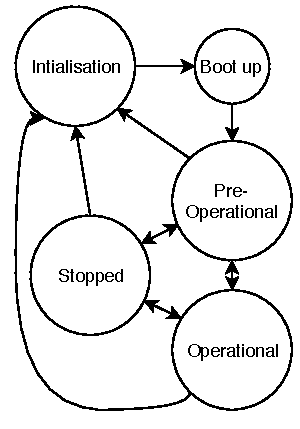
\includegraphics[width=0.3\textwidth]{figures/CANOpen_NMT}
    \end{center}
    \vspace{-0.5cm}
    \caption{Device states described in CANOpen specification}
    \label{fig:CANOpen NMT}
\end{wrapfigure}
Beside exchange of data CANOpen protocol describes a way to control basic device states. By messages referred as "Network Management" (NMT) one can read device state and send commands to change it. The states and all possible transitions are shown in figure \ref{fig:CANOpen NMT}.

As one can notice to states are restricted to ones important for communication and parameters setting. After the device is on, booting sequence can be started then in a pre-operational state all configuration can be made to finally turn it into operational mode. For instance in connecting to a motor controller, firstly we check communication then turn on pre-charge circuit during boot sequence then setup all necessary parameters (encoder, current limitation etc.) subsequently turning the control loop on.

This is just cover general states but in more complex applications clearly, there are more states to address, however, in this case, there is nothing stopping us from using certain objects in the dictionary to control sub-states.

Last but not least, there are 4 more functions cover: Emergency (EMC) - responsible for asynchronous communication of errors, previously mentioned SYNC - to periodically request device state, time stamp - to synchronise devices clock and layer settings services (LSS) - to automatically identify multiple devices on the bus.

All these briefly described functions, collectively provide powerful abstraction over the CAN network standardising way it is used.

\cite{CAN_CIA,CANOpen_NIKHEF,CANOpen_solutions,CANOpen_microcontrol}
\\ \\ \\ \\ \\ \\ 

% \section{Steering - torque vectoring and load sharing}


% \chapter{Existing solutions/ compare to IC vehicles}
% Literature review on recent developments within the topic and techniques used in combustion engine cars
%!TEX root = ../Thesis.tex

% 1.2 Defining the scope of your thesis
% One of the first tasks of a researcher is defining the scope of a study, i.e., its area (theme, field) and the amount of information to be included. Narrowing the scope of your thesis can be time-consuming. Paradoxically, the more you limit the scope, the more interesting it becomes. This is because a narrower scope lets you clarify the problem and study it at greater depth, whereas very broad research questions only allow a superficial treatment.

% The research question can be formulated as one main question with (a few) more specific sub-questions or in the form of a hypothesis that will be tested.

% Your research question will be your guide as your writing proceeds. If you are working independently, you are also free to modify it as you go along.

% How do you know that you have drafted a research question? Most importantly, a research question is something that can be answered. If not, you have probably come up with a theme or field, not a question.

% Some tips:

% Use interrogative words: how, why, which (factors/situations) etc.
% Some questions are closed and only invoke concrete/limited answers. Others will open up for discussions and different interpretations.
% Asking “What …?” is a more closed question than asking “How?” or “In what way?”
% Asking “Why” means you are investigating what causes of a phenomenon. Studying causality is methodologically demanding.
% Feel free to pose partially open questions that allow discussions of the overall theme, e.g., “In what way …?”; “How can we understand [a particular phenomenon]?”
% Try to condense your research question into one general question – and perhaps a few more specific sub-questions (two or three will usually suffice).

\section{Scope of the thesis}
In my perception the scope of this thesis was greatly expanding over the time. I started with simple question of "How the torque vectoring/load balancing can be implemented in electric car?". This question however could be addressed in two ways, one would be by a theoretical divagations, second by practical implementation details.

Since it was a first time when DTU is participating in Formula Student competition, I could not work on already working solution from previous years.
Therefore, the objective of the thesis was in great manner implementation oriented and difficulty moved towards all small design decisions, each base subsystem and cooperation with independent teams. So I would actually put the twist on the original question: "How to implement maintainable, performant and safe electric car control system in the manner that it would be additionally able provide torque vectoring functionality?".

In the following chapters, I will try to explain my design decisions their advantages, drawbacks and how they builds up a complete control system.
%!TEX root = ../Thesis.tex

% 1.3 Outline
% The outline gives an overview of the main points of your thesis. It clarifies the structure of your thesis and helps you find the correct focus for your work. The outline can also be used in supervision sessions, especially in the beginning. You might find that you need to restructure your thesis. Working on your outline can then be a good way of making sense of the necessary changes. A good outline shows how the different parts relate to each other and is a useful guide for the reader.

\section{Outline}
This thesis consist of \ref{total:chapters} chapters. It starts with the general introduction you are reading now, which outlines topic of the work being done.
%, hopefully giving pleasant to read opening. 

In the next chapter, knowing current state of art and being aware of the limitations I have written theoretical considerations. They are base for the implementation part as well as a reference point for analysing and discussion.

It has been followed by description of the design process in chapter 3. Which naturally evolves into methods being implemented in final stadium described in chapter 4. In this chapter I have placed a comprehensive description of my design choices, used setup and implementation itself. This part is directly followed by information of how I did test my system and how well it performs against my theoretical considerations.

Then I let myself describe directions for the future implementation which I hope will come in handy for future teams taking care of this project.

A whole text is closed with a few closing comments from me, retrospection on the whole process of building an electric racing car and my part in it.

\todo{Delete rest?}
Beside the mentioned hierarchy, it has been formed to follow two additional nested level. In each chapter, the following sections are sorted in the way to reflect the propagation of CAN messages in the system.

\begin{figure*}[h]
    \centering
            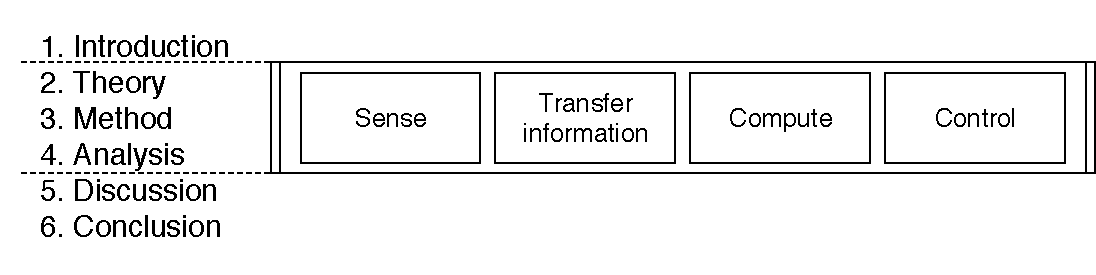
\includegraphics[width=0.8\textwidth]{figures/Outline}
            \label{outline}
            % \caption{CAN and CANOpen timing overview}
\end{figure*}
%!TEX root = ../Thesis.tex

% 2. Theory section
% The theory used in an empirical study is meant to shed light on the data in a scholarly or scientific manner. It should give insights not achievable by ordinary, everyday reflections. The main purpose of using theory is to analyse and interpret your data. Therefore, you should not present theoretical perspectives that are not being put to use. Doing so will create false expectations, and suggests that your work is incomplete.

% Not all theses have a separate theory section. In the IMRaD format the theory section is included in the introduction, and the second chapter covers the methods used.

% What kind of theory should you choose? Since the theory is the foundation for your data analysis it can be useful to select a theory that lets you distinguish between, and categorise different phenomena. Other theories let you develop the various nuances of a phenomenon. In other words, you have a choice of either reducing the complexity of your data or expanding upon something that initially looks simple.

% How much time and space should you devote to the theory chapter? This is a difficult question. Some theses dwell too long on theory and never get to the main point: the analysis and discussion. But it is also important to have read enough theory to know what to look for when collecting data. The nature of your research should decide: Some studies do not require much theory, but put more emphasis on the method, while other studies need a rich theory section to enable an interesting discussion.

\chapter{Theory}

\section{Calculations for differential based on steering angle} \label{diff_calc}

Due to the racing character the vehicle were build with parallel steering mechanism. Considering the dynamics of the vehicle in high speeds during the turn the outer wheel works under presumably higher load therefore having smaller slip angle than relieved inner wheel. In well designed parallel steering system these forces should cancel each other therefore we can make the calculations based on two wheels model with unchanged steering angle \todo{bike model}.
In this model we can simply calculate the radius of turn measuring from rear axle by trigonometric equation $Rear axis turn radius = cot( steering angle ) * wheelbase$. Now moving back to four wheel model, since the radius is directly proportional to circumference we can calculate the proportions of how fast should wheels rotate in compare to consider rear wheel from previous model. This can be done by simply adding half of rear track to calculated radius and divide by it.
\begin{equation}
    inner wheel proportional speed = \frac{rear axis radius - rear track / 2}{rear axis radius}
\end{equation}
\begin{equation}
    outer wheel proportional speed = \frac{rear axis radius + rear track / 2}{rear axis radius}
\end{equation}
These numbers can be successfully used as multiplicands in differential system for either torque or speed control loops.

\section{Regenerative Breaking} \label{regenerative_theory_section}

As explained in \cite{low_speed_regenerative_breaking} and confirmed in \cite{regen_strategy} it is not feasible to use the regenerative breaking for the vehicle driving with the low speed. As the motors would generate to small voltage to be converted up and charge the battery.
%!TEX root = ../Thesis.tex

% 3. Method section
% In a scholarly research article, the section dealing with method is very important. The same applies to an empirical thesis. For students, this can be a difficult section to write, especially since its purpose may not always be clear.

% The method chapter should not iterate the contents of methodology handbooks. For example, if you have carried out interviews, you do not need to list all the different types of research interview. You also do not need to describe the differences between quantitative and qualitative methods, or list all different kinds of validity and reliability.

% What you must do is to show how your choice of design and research method is suited to answering your research question(s). Demonstrate that you have given due consideration to the validity and reliability of your chosen method. By “showing” instead of “telling”, you demonstrate that you have understood the practical meaning of these concepts. This way, the method section is not only able to tie the different parts of your thesis together, it also becomes interesting to read!

% Show the reader what you have done in your study, and explain why. How did you collect the data? Which options became available through your chosen approach?
% What were your working conditions? What considerations did you have to balance?
% Tell the reader what you did to increase the validity of your research. E.g., what can you say about the reliability in data collection? How do you know that you have actually investigated what you intended to investigate? What conclusions can be drawn on this basis? Which conclusions are certain and which are more tentative? Can your results be applied in other areas? Can you generalise? If so, why? If not, why not?
% You should aim to describe weaknesses as well as strengths. An excellent thesis distinguishes itself by defending – and at the same time criticising – the choices made.

\chapter{Method}

% Having not sufficient financial support enforced many compromises on design which I did not have direct influence on. The decision was made that will be running in low voltage - high current setup so we could use cost-efficient lithium-ion batteries. 
% Although theoretically possible cabling and connector sizing was a bit overwhelming for responsible teams.


\begin{figure}[b]
	\centering
    	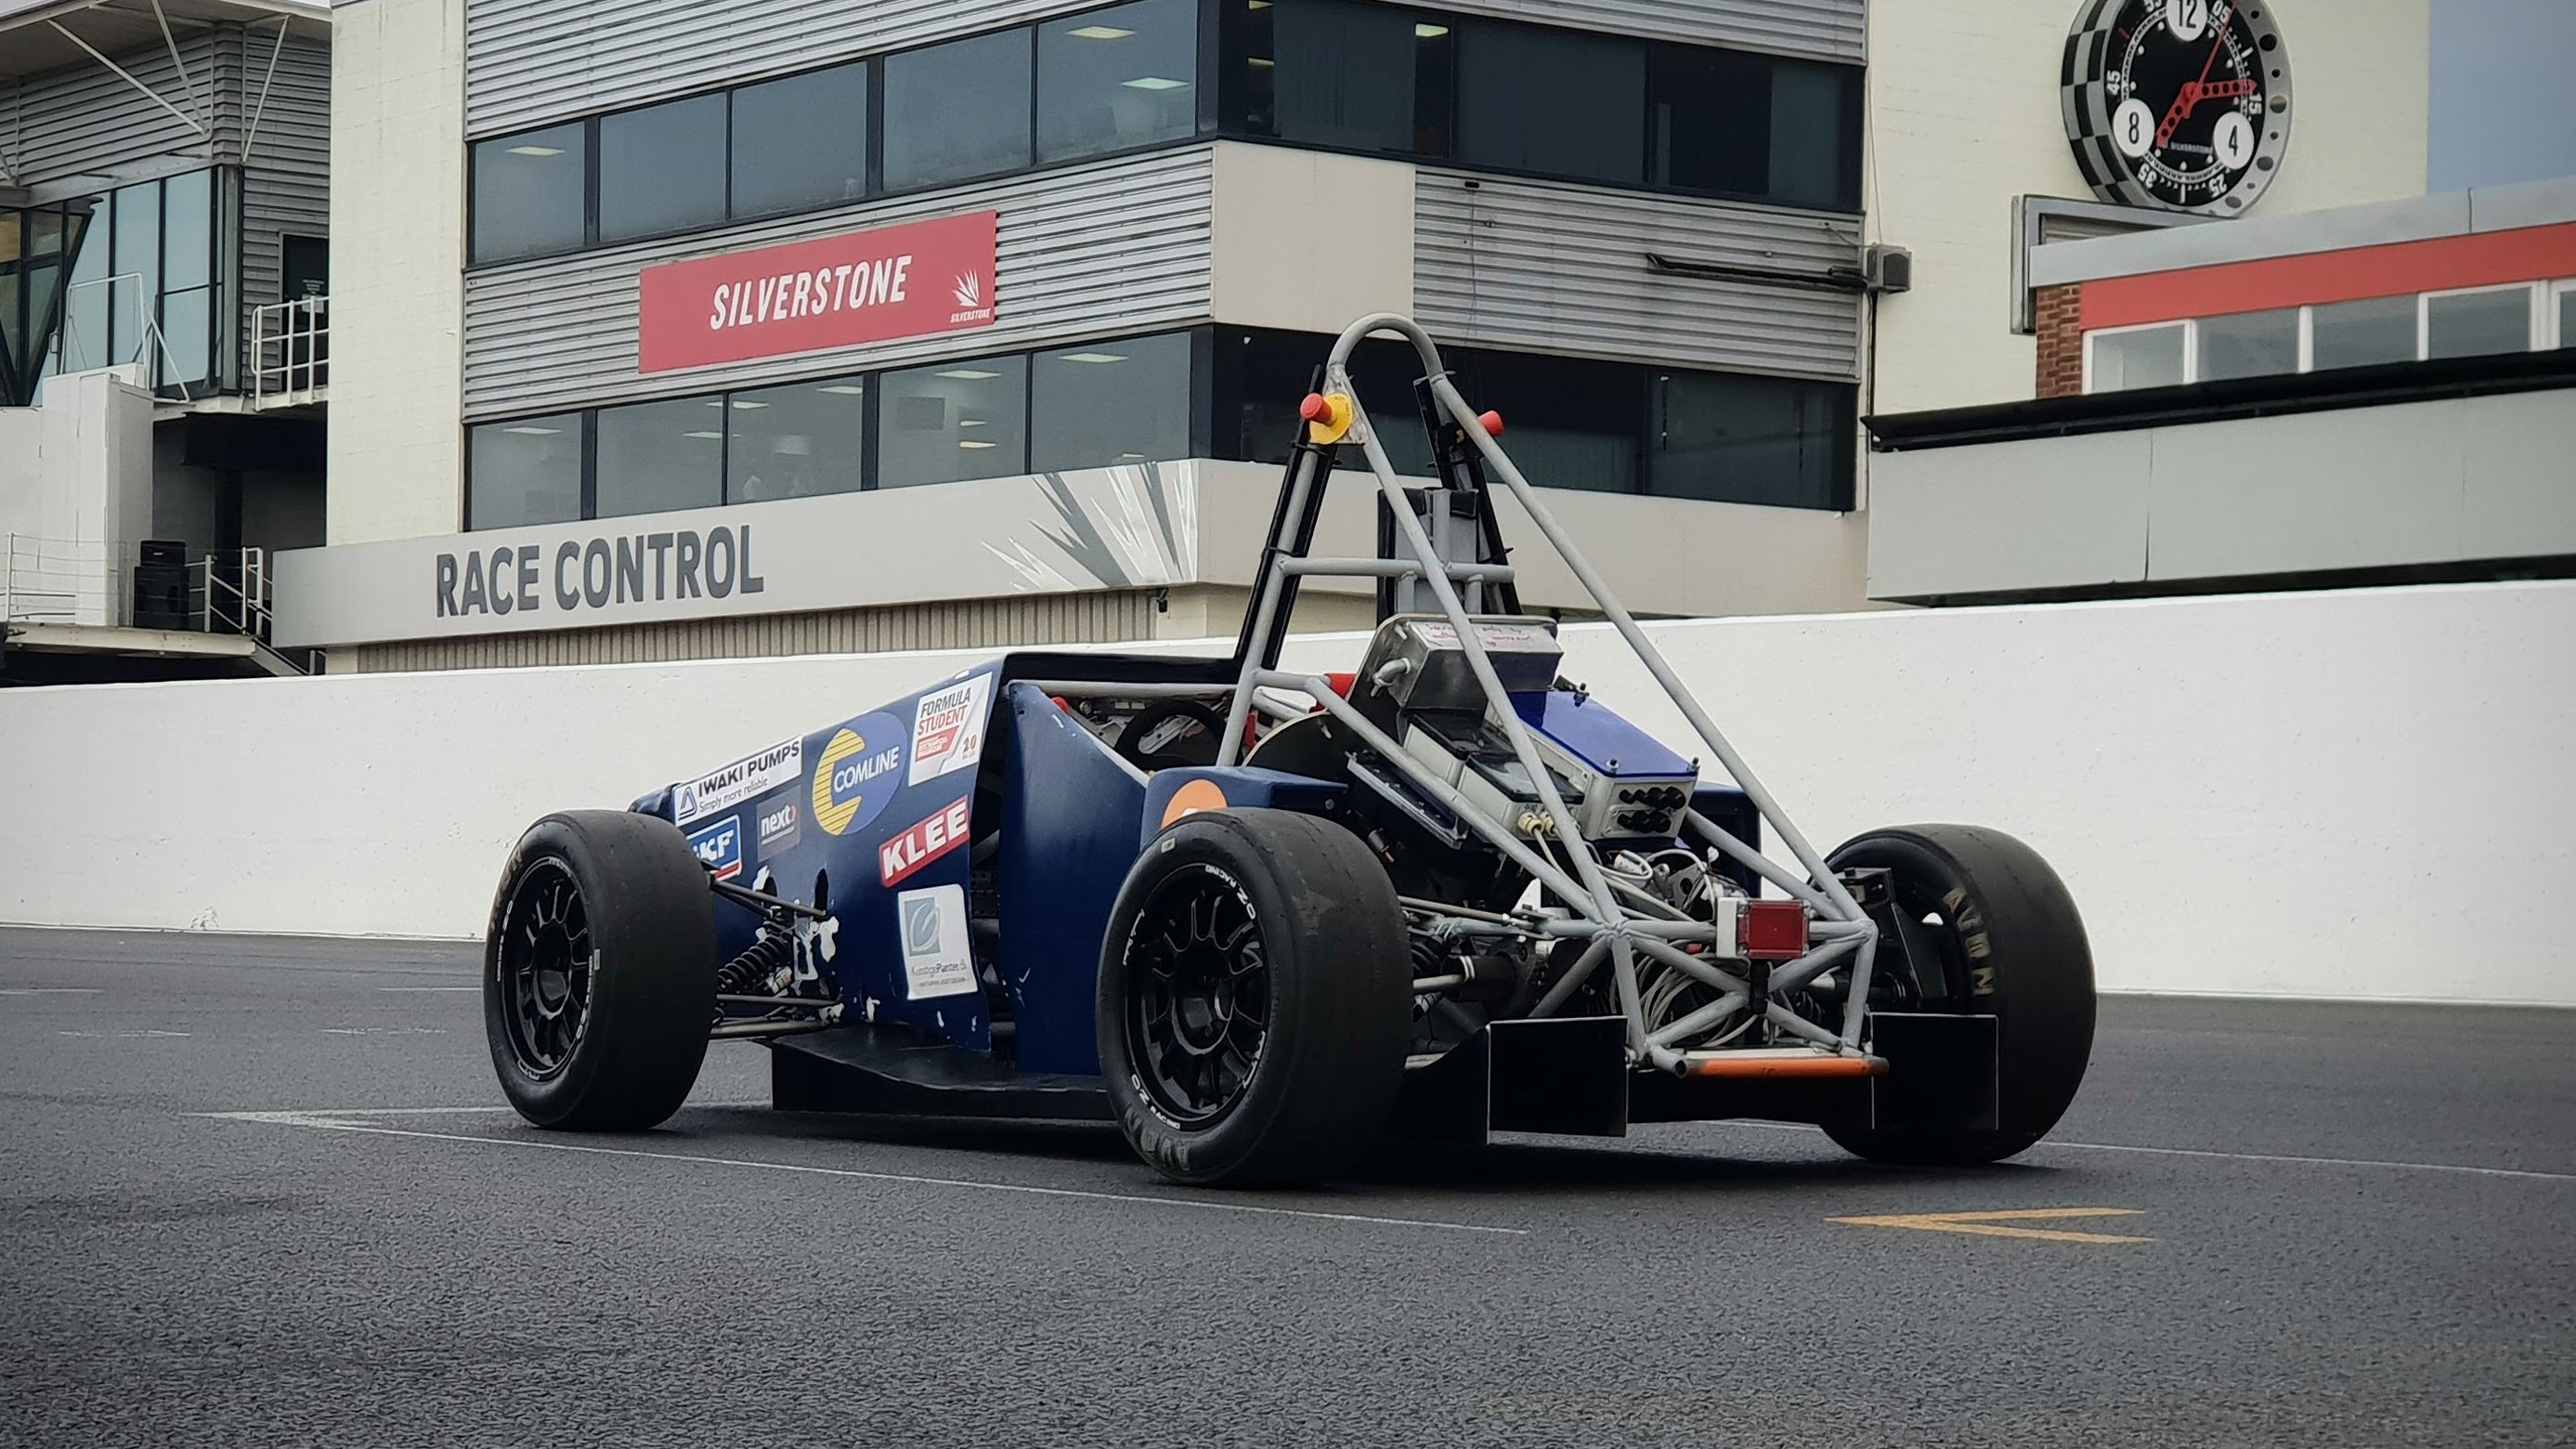
\includegraphics[width=0.8\textwidth]{figures/silverstone.jpg}
        \caption{Built car on Silverstone race circuit}
        \ref{pic:silverstone}
\end{figure}


We\todo{is it right to say we?} have built an electric car from scratch based on buggy frame, where all the pipes are welded together and all the components directly attached to it. Although in this solution, all the vibrations are transferred to the driver (reducing his comfort) it is a durable and light solution - the aspects which were the most important due to the racing character of the vehicle. 

In our final setup we used:
\begin{itemize}
    \item Two EMRAX228 motors which nominal power of about 50kW (when liquid cooled)
    \item Two emDrive500 controllers capable full usage of AM motors
    \item Arduino with CAN shields to act as intelligent sensors/controllers
    \item Two \todo{which pumps? Iwaki direct drive pump rd-40e24-hn1v} pumps for cooling purposes
    % \begin{wrapfigure}
    %     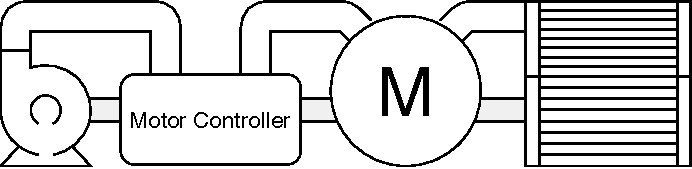
\includegraphics[width=0.33\textwidth]{figures/Pump.pdf}
    % \end{wrapfigure}
    \item National Instruments' cRIO-9033 as a main control unit
\end{itemize}

This result in the system which in a simplified manner has been presented in figure \todo{figure ref}.

\todo{figure}

As shown all the communication with the master control unit is based on CAN bus. 






All small subsystems are based on Arduino evaluation boards.




As previously mentioned the main control unit has been deployed on cRIO9033 - National Instruments' controller equipped with a real-time processor and re-configurable FPGA unit. The reasoning for usage of this device was that it has more than sufficient computation power for the task and with additional modules provides support for basic CAN communication as well as high-level CANOpen abstraction.


In my setup, I have been using module NI9853 to directly receive and send a CAN messages and NI9881 for communication with the motor controllers based on CANOpen standard.

\section{Master control unit software implementation}
From the early beginning, I have been developing the code of master control unit using event-based programming paradigm. The reasoning of this is asynchronous, real-time nature of such unit.

Most simple classification of subsystems can be based on communication protocol being used. 

\subsection{Communication protocols}

\subsubsection{CAN integration}
To start with I had to implement a CAN library which would let me service messages from the code running on the real-time processor. I did it based on one of the provided examples, however, to meet my needs it required some ground modifications.

Especially functionality which has been missing is the ability to wait for a message with a certain id, one from an array of ids or just any message. 
\paragraph{Reading}

To achieve it, I have a functionality deployed on FPGA (Field Programmable Gate Array) which simply translates input/output messages into the arrays of 8x unsigned integers. Read messages are furthermore pushed into the FIFO register. In parallel, a consumer process is running which takes messages from the register set it as an output and raise an interrupt on the real-time processor to notify that data is ready to be read.

Upon initiation of the device, a programme is run on the real-time processor which beside the main process spawns an additional one in the background. This one furthermore is responsible for communication with the FPGA so whenever a message arrives it services interrupt by copying it and sends the acknowledge back to FPGA so next one can be transmitted. Meanwhile, CAN frame is stored in the table indexed by its ID and two notifications are sent (for the desired frame and for the arrival of any message)\footnote{Usage of LabVIEW synchronisation primitive "Queue" further described in \todo{queue description}}.

Now depending on a place in the code read function can be called in one of three ways:
\begin{description}[labelindent=1cm]
    \item[Read All] - function blocks the thread until notification arrives that any message has been received (or upon timeout) and returns it. Example of usage would be a logging purpose.
    \item[Read Some] - for given list of message IDs function behaves similarly to "Read All". However, notification is read and check if contains one of the listed IDs if not it starts again and return frame upon success (or error upon timeout). Example - Error handler.
    \item[Read ID] - waits for notification associated with the certain ID. Example - read pedal position.
    
%     Then look up table is check for the existence of a conditional variable for given id, it is created if does not exist, and updated with a new message. Additionally, a conditional variable containing the id of last received message id is updated.

% Based to this architecture I implemented functions which can wait for any message, one with a certain id or one from ids set.

\end{description}

\paragraph{Writing}
For sending a message it simply pushes data to FPGA and marks it as ready to send. FPGA is constantly checking the ready to send status and whenever it becomes true sends the data.

\vspace{5mm}
\noindent Thank\todo{seriously without to!?} this architecture CAN messaging part is easy to use, read and modify.

\subsubsection{CANOpen}
For the simplicity and maximum throughput although CANOpen is an abstraction layer over CAN bus an additional line has been used only for CANOpen communication. It has been used just to link two motor controllers and NI-9881 module (plugged into cRIO).

For the usage, CANOpen seemed like the best choice. It provides great flexibility in the way that all parameters can be accessed the way as they would be stored in memory registry without any pre-configuration. Furthermore, if setup correctly certain number of parameters can be accessed without any protocol overhead providing maximum bus throughput.

As previously mentioned in \todo{where} CANOpen abstraction consists of 6 complementary sub-protocols.
\begin{description}[labelindent=1cm]
    \item[NMT] Network management - Provides unified control over the devices state (Boot up, Pre-operational, Operational, Stopped)
    \item[SDO] Service Data Object - verbose protocol by default providing access to all the parameters of the device, it works based on two messages schema first describing which data should be sent next then in second sending actual data
    \item[PDO] Process Data Object - configurable sets of parameters to send/receive upon change or after SYNC message
    \item[SYNC]	Synchronisation Object - issue request of device status
    \item[TIME]	Time Stamp Object - is used to synchronise with device clock and it had no use in this project
    \item[EMCY] Emergency Object - asynchronously broadcast errors
\end{description}

As it meant to be I implemented one drive control based on NMT, SDO, PDO and SYNC protocols. Using NMT to control general state, SDO to control all the parameters before setting the device into operational mode and control device-specific states and PDO combined with SYNC messages to read device status and send control messages.

However, as it came to controlling two motors simultaneously conflicting messages ids in PDO and SYNC protocols needed to be changed. Although many tries it was not possible to change this values. Contacting the manufacturer drop the light on the case as they were aware that their devices malfunctions and were not able to provide any fix for the issue.

So for the two motor configuration, I had to implement a workaround by using slower and not providing all the functionality SDO protocol.
Usage of this protocol caused a drastic drop in channel throughput considering for instance reading of device status:
\begin{table}[H]
\centering
\begin{tabular}{|l|c|}
    \hline
    Data & Data size [byte] \\
    \hline
    Status word & 2 \\
    Controller Temperature & 1 \\
    Motor Temperature & 1 \\
    Error Code & 2  \\
    Error Register & 1 \\
    Torque Actual Value & 2  \\
    Velocity actual Value & 4  \\
    Electrical Angle & 2  \\
    Electric Power & 4 \\
    \hline
    \hfill Sum & 19 \\
    \hline
\end{tabular}
\caption{Motor controller status component sizing}
\end{table}

As each PDO message can contain up to 8 bytes aforementioned list of parameters would need to be divided into 3 CAN frames and as an result $46bits*3+19bytes+\epsilon = 290 bits +\epsilon$  \hspace{0.2cm}\footnote{\label{foot:eps}$\epsilon$ has been used to represent stuffed bits} needs to be send. On the other hand sending the same data with SDO protocol requires request-respond schema for each value so $46bits*18 + 19bytes + 9*4bytes + \epsilon = 1268 bits + \epsilon$ \hspace{0.2cm} \ref{foot:eps} needs to be send.

\begin{figure}[h]
    \centering
    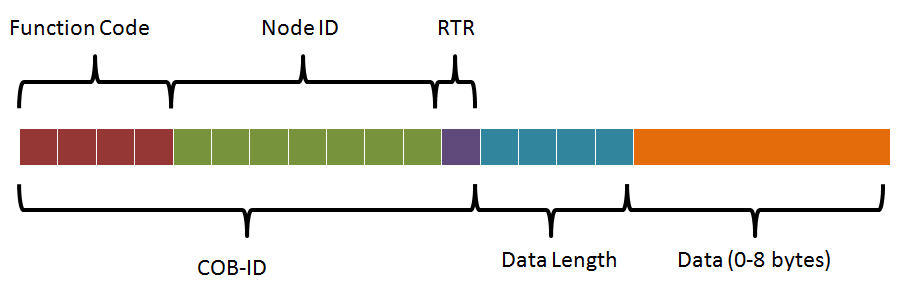
\includegraphics[width=0.8\textwidth]{figures/CANOpen vs CAN.png}
    \caption{CANOpen vs CAN}
    \label{fig:canopen_bitwise}
    \todo{enrich it by missing fields}
\end{figure}

Furthermore, also the target torque off motor controllers needs to be adjusted SDO messages. In this case performance drawback is even more visible, if the PDO protocol could be used torque values could be sent together within one CAN frame ($46bits+4bytes=78 bits$), however, within SDO 4 CAN frames needs to be sent ($46bits*4+4bytes+4bytes*2=280bits$).

\subsection{Device operation states}

\begin{wrapfigure}{R}{0.43\textwidth}
    \vspace{-20pt}
    \begin{center}
        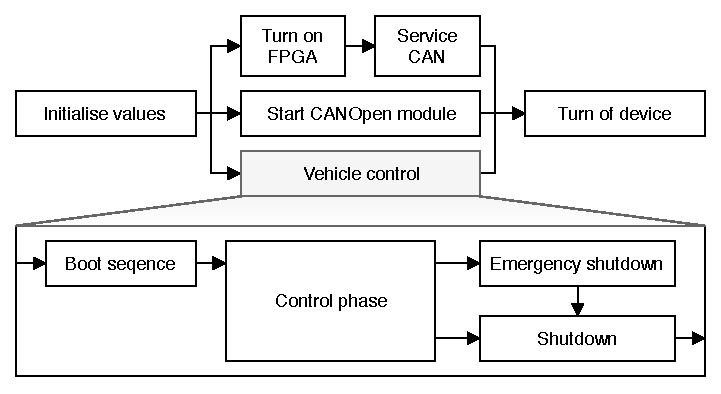
\includegraphics[width=0.4\textwidth]{figures/System_overview}
        \label{fig:sys_over}
        \caption{Control unit\newline states overview}
    \end{center}
    \vspace{-20pt}
\end{wrapfigure}

Implemented control unit in practice consist of few nested state machines. The most general consist of just 3 states responsible for controller booting, operational and shutdown.
In booting state all initial values are set and internal modules like FPGA, CAN and CANOpen are being turned on in parallel to main threads. Whenever, this phase is finished, error logger is turn on and car booting sequence begins.

To start with, the dashboard is updated with batteries charge status and systems waits for power up button to be pressed. Whenever driver would command turning of the vehicle button blinks and lights up by internal LED whenever BMS would response with ready to discharge message. Then second button is required to be pressed in order to turn the traction system on (analogical interface to first button). Whenever traction system is first turned on, controller sends message to audio-visual system so the car plays loud sound alerting the surrounding to take cautions as systems are charge and it is ready to drive.

In operational state many control loops runs in parallel to cover desired vehicle functionality.
\begin{itemize}
    \item Pedals status is read, updates local pedal status and issue notification that motor controllers should be updated with new values. 
    \item Upon notification new target torques values are calculated and send to motor controllers.
    \item Running watchdog, if no pedals update was notified within 500ms set target torques to zero (emergency mechanism to slow the motors in case of any temporary fail of pedals sensor).
    \item Set pumps to full power for 3s to initiate rotation, then control it accordingly to further mentioned method.\ref{pump_control}
    \item Communicate with BMS to keep it in operational state.
    \item Read and act upon BMS and low voltage BMS state.
    \item Log all the information.
\end{itemize}


\section{Pedals sensor}
A System to measure pedals and steering wheel position is based on Arduino evaluation board. Which is a simple evaluation setup build upon Atmel ATmega8 with $16MHz$ oscillator.

Now considering the sampling rate of this sub-module it has been programmed to use prescaler for A/D converter with a value of 128. Referring to datasheet basic conversion takes 13 clock cycles so we should except sampling rate of about $16MHz/128/13 = 9615Hz = 104µs$ \cite{Atmega8}.

However, in an electric car, there is a considerable electromagnetic noise which needs to be addressed. To reduce the impact of noise which was significant in the first approach, the code was modified to calculate an average of 10 successive samples efficiently reducing the rate to $1,04ms$.

Considering the fact that ATmega8 consist of just one analogue-decimal converter with multiplexed input the measurement takes approximately $1,04ms * number of sensors$ \cite{Atmega8}.
To satisfy the safety requirements we needed to use two offset sensors for each pedal (accelerator, brake) and one for the steering wheel. In consequence each measurement takes at least $1,04ms * 5 = 5,2ms$.

This system sense all the information which is:
\begin{itemize}
    \item pedals position
    \item steering wheel position
    \item pedals sensors position miss-match
    \item pedals, steering wheel over-travel, under-travel and connection loss errors
\end{itemize}

After the measurement, the information is sent through CAN bus with a baud rate of 500kbit/s (used CAN module was not capable to work with higher baud rates). Pedals position although being read on 10 bits is averaged and only 8 significant bits are sent. We assumed that 256 quantization steps are sufficient in this case. It allowed us to shorten CAN frame to consist of only 4 bytes of data.
Now considering timing, the CAN frame (\todo{CAN frame graphic (wiki like)}) consists of 44 basic bits plus 4 bytes of data in our case. The total time of sending/receiving would be therefore $\frac{76}{500kbit/s} = 152us$.

Assuming no further improvements we should expect the pedals sub-systems is capable of sending the pedals, steering wheel position in a time interval of about $5,2ms$\label{pedal_ideal_time} in normal operation.
Additionally, if any of the above-mentioned errors occurred the second CAN frame is sent containing two bytes with bitwise encoded errors extending the expected interval into $~5,3ms$.

\section{Pump control}\label{pump_control}
In our car, we have used \todo{which pump} pumps, which can be controlled by a signal from $0-5V$. Since used Arduino has no dedicated analogue input we made one by using the PWM signal with a low-pass filter (direct control by PWM signal was strongly disapproved by the pump manufacturer \todo{cite pump manual}).
The subsystem acts simply by controlling pulse width based on the value received by CAN message from the master control unit. It also provides basic emergency behaviour in the manner that if no message was sensed over one second the pumps are turned on to work with full power.






\section{Implementation of electrical differential based on steering angle}\label{diff_meth}
In my implementation I have enriched calculations explained in \ref{diff_calc}. Starting with the steering wheel, the sensor output is normalised to the measured minimum and maximum steering wheel angles ($\pm123\deg$) so the meaningful value can be shown in remote control panel as well as saved in logs. 
Then since it is linearly proportional it is simply converted to steering angle ($\pm35\deg$). To prevent any miss usage all the values are coerced on the go to be within the ranges.

Having commanded output power (in percentage) basic differential functionality could be obtained just by multiplying it with a maximum allowed/available torque and proportion on per wheel base. However, it would start failing for power close to $100\% $, although total torque will remain under the limit, the outer wheel can go above the limit by up to ($20\% $).
This situation would be especially dangerous if the maximum torque per wheel base would start to saturate. In this case the differential would gradually stop to function effectively pushing the car out of the desired curve.
To avoid this miss-behaviour I added the code to check if after previous calculation any of the wheels is about to be set to more than maximum torque and scale both of them accordingly.
\begin{equation}\label{diff_saf}
    \tau_{left,right} = \begin{cases}
        \tau_{left,right} = P * \gamma_{left,right} * \tau_{max} & \text{se $m(P,\gamma_{left,right}) \leq 1$}\\
        \tau_{left,right} = P * \gamma_{left,right} * \tau_{max} / m(P,\gamma_{left,right}) & \text{se $m(P,\gamma_{left,right}) > 1$}\\
    \end{cases}
\end{equation}
Where:
\begin{description}
    \item[P] desired output power ($0-100\%$)
    \item[$\tau_{max}$] maximum torque per wheel
    \item[$\tau$] wheel torque
    \item[$\gamma$] differential disproportion of wheel ($\gamma_{left}+\gamma_{right}=200\%$)
    \item[$m(P,\gamma{left,right})$] $= P * max(\gamma_{left},\gamma_{right})$
\end{description}

\section{Regenerative braking}
As mentioned in theory chapter (\ref{regenerative_theory_section}) the regenerative braking cannot be used in low speeds. Normally this problem would be solved by varying the braking force between regenerative and friction breaks. However, the car design did not take into the account possibility to electrically control the friction breaks. So I implemented an alternative solution taking into account this technical obstacle and comfort of the driver.
Considering regenerative braking as negative torque system which I have implemented can be expressed by equation \ref{reg_break_eq}.


\begin{equation*}
    \tau = \begin{cases}
        D & \text{se $V_{avg} \leq 10km/h$}\\
        (V_{norm,10-20} * 15\% + 100\%) * D - V_{norm,10-20} * 15\% & \text{se $V_{avg} \in (10km/h,20km/h>$}\\
        115\% * D - 15\% & \text{se $V_{avg} > 20km/h$}\\
    \end{cases}
    \label{reg_break_eq}
\end{equation*}
Where:
\begin{description}
    \item[$V_{avg}$] average velocity of the wheels 
    \item[$V_{norm,10-20}$] $V_{avg}$ normalised in range from 10 to 20 ($V_{norm,10-20}=(V_{avg}-10)/10$)
    \item[D] acceleration pedal displacement in percentage
    \item[$tau$] percentage of used torque (in reference to maximum value)
\end{description}

It follows the simple idea to use variable portion of pedal displacement for regenerative braking based on speed.
When the user presses acceleration pedal in stationary vehicle the whole available scale is used to control torque giving expected instant response. After reaching $10km/h$ the pedal  displacement used for regenerative braking increases gradually to reach $15\%$ while travelling with speed equal or higher than $20km/h$.
What else is worth to mention is that as a result for the pedal displacement from $0-15\%$ we should expect the car to act as it would be controlled in speed mode.\label{speed_mode} The characteristic would be firstly saturated by low torque however within enough power to make the car accelerate we should be able to observe linear correlation between pedal displacement and speed.
To summarise the expected idealised correlation between torque, pedal displacement and speed has been shown in figure \ref{regen_ideal}.

\begin{figure}[h]
    \centering
        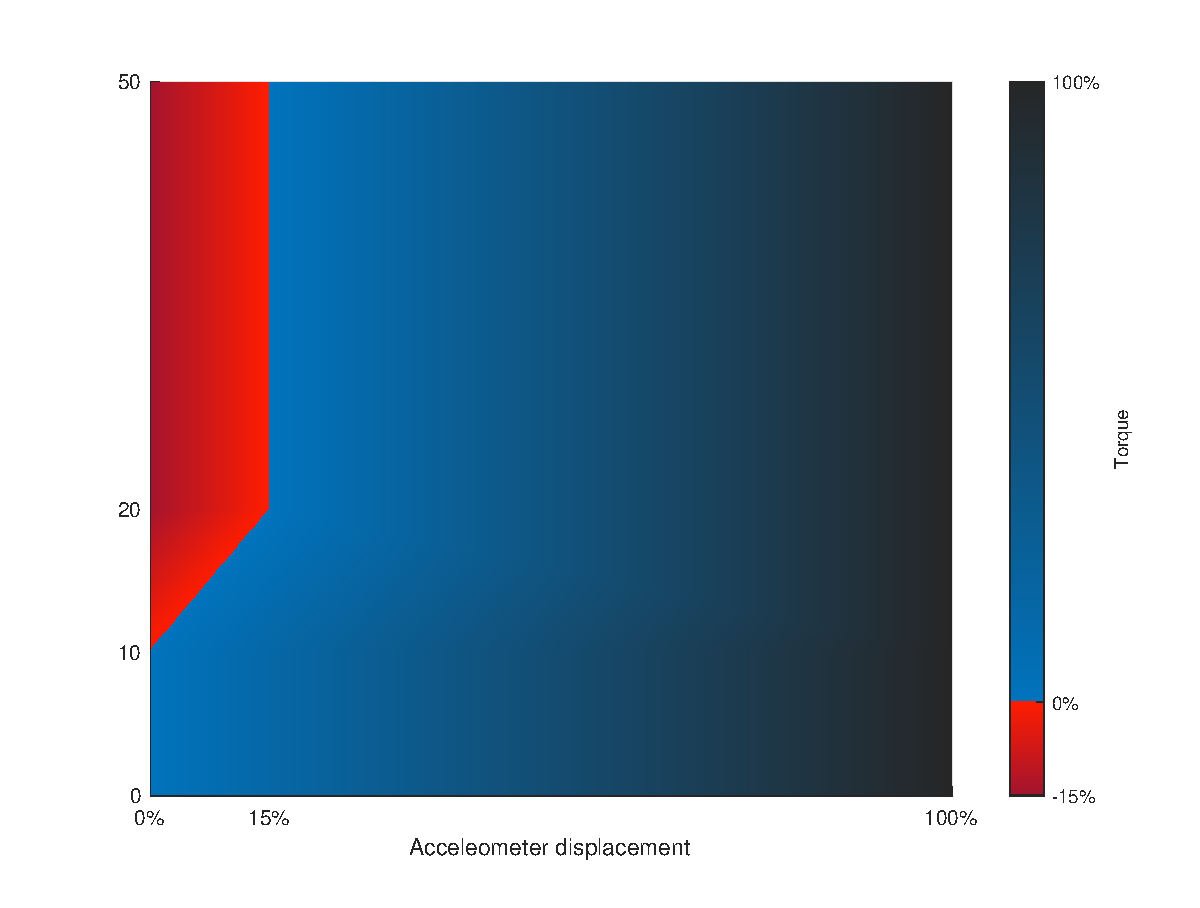
\includegraphics[height=5.8cm]{figures/regen_ideal}
        \caption{Regenerative braking / torque control}
        \label{regen_ideal}
\end{figure}





%!TEX root = ../Thesis.tex

% 4. Analysis
% Your analysis, along with your discussion, will form the high light of your thesis. In the IMRaD format, this section is titled “Results”. This is where you report your findings and present them in a systematic manner. The expectations of the reader have been built up through the other chapters, make sure you fulfil these expectations.

% To analyse means to distinguish between different types of phenomena – similar from different. Importantly, by distinguishing between different phenomena, your theory is put to work. Precisely how your analysis should appear, however, is a methodological question. Finding out how best to organise and present your findings may take some time. A good place to look for examples and inspiration is repositories for master’s theses.

% If you are analysing human actions, you may want to engage the reader’s emotions. In this case, it will be important to choose analytical categories that correlate to your chosen theory. Engaging emotions is not the main point, but a way to elucidate the phenomenon so that the reader understands it in a new and better way.

% Note: Not all theses include a separate chapter for analysis.

\chapter{Analysis}

\section{Pump control}
To check the declared functionality of pump control I have made a test setup where motor's thermoresistors can be replaced with matched potentiometers. In this manner, I could fully control the temperatures sensed in the very beginning of the system and what is important without any modifications to the final version of the software.
\newline
\newline
I have captured 10 state transitions to demonstrate the whole spectrum of changes as follows.
\begin{description}
    \item[Temperature set to 30\textdegree C and varying accelerator displacement] \hfill \\ Expected behaviour of pumps output would be to raise proportionally from 2,5V for pedal in initial position up to 5V whenever it is pressed up to its limit.
    \item[Temperature set to 35\textdegree C and varying accelerator displacement] \hfill \\ Same behaviour as explained above.
    \item[Temperature set to 40\textdegree C and varying accelerator displacement] \hfill \\ Same behaviour as explained above.
    \item[Temperature set to 45\textdegree C and varying accelerator displacement] \hfill \\ Initial pump output should equal to $2,5V + 2,5V*25\% = 3,125V$ and saturate on pedal displacement of $75\% $.
    \item[Temperature set to 50\textdegree C and varying accelerator displacement] \hfill \\ Initial pump output should equal to $2,5V + 2,5V*50\% = 3,75V$ and saturate on pedal displacement of $50\% $.
    \item[Temperature set to 55\textdegree C and varying accelerator displacement] \hfill \\ Initial pump output should equal to $2,5V + 2,5V*75\% = 4,375V$ and saturate on pedal displacement of $25\% $.
    \item[Temperature set to 60\textdegree C and varying accelerator displacement] \hfill \\ Initial pump output should equal to maximum value of $5V$ and pedal displacement should not affect this value.
    \item[Temperature set to 65\textdegree C and varying accelerator displacement] \hfill \\ Same behaviour as explained above.
    \item[Temperature set to 70\textdegree C and varying accelerator displacement] \hfill \\ Same behaviour as explained above.
\end{description}
\begin{description}
    \item[Varying temperature from 30 to 70 degrees and no accelerator displacement] \hfill \\ Pump output should vary from $2,5V$ and $5V$ being in direct proportion to temperature changes from 40 to 60 degrees.
\end{description}

Taking for instance measurement for temperature set $50\deg C$ and pressing acceleration pedal. I have had captured extremely noisy signal from accelerator sensor and temperature sensor emulator then prepossessed in a similar manner as it is done inside the system (just to filter out the electromagnetic noise \todo{Precise description?}). The sensors output, as well as pumps controlling signal, has been shown in the figure \ref{pump_50}.

\begin{figure}[h]
    \centering
    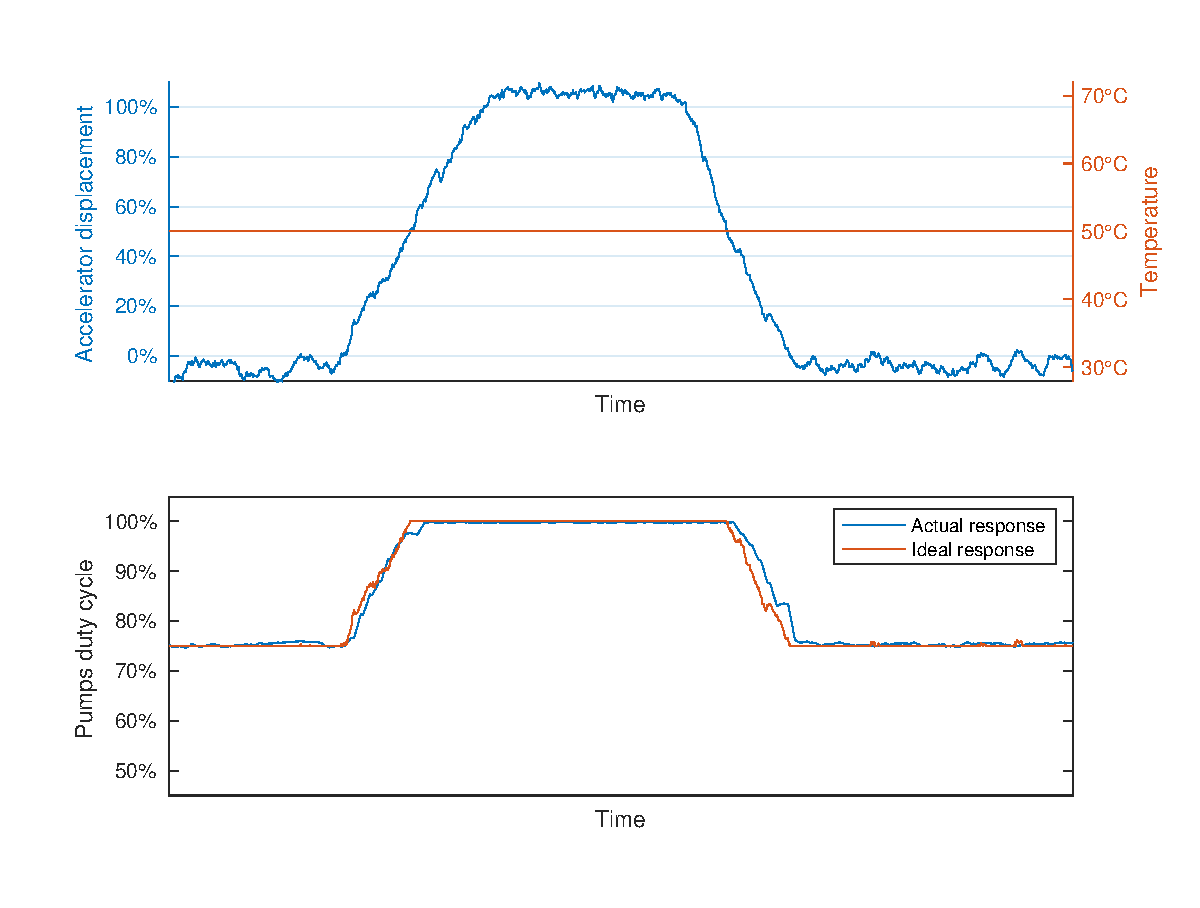
\includegraphics[height=5.8cm]{figures/pump_50.eps}
    \caption[Temperature set to 50\textdegree C and varying accelerator displacement]{Comparison of actual pump control signal to idealised one based on the same input data}
    \label{pump_50}
\end{figure}

In the same figure, I have plot theoretical output based on an idealised mathematical model. As one can notice control output closely follows the desired patch. The only visible difference is due to the fact that in my system the control signal is intentionally delayed.
The pumps control signal is updated only once per 100 milliseconds since temperature change is rather a slow process in this way we can avoid harmful (for pumps) high-frequency oscillations and save computation power. In this way, we obtain a simple control system with memory which is even more visible if we just plot input against output (accelerator/control signal) which has been done in \ref{pump_50_1}. In the graph, we can observe the hysteresis and steps upon control update as we could expect.


\begin{figure}[h]
    \centering
    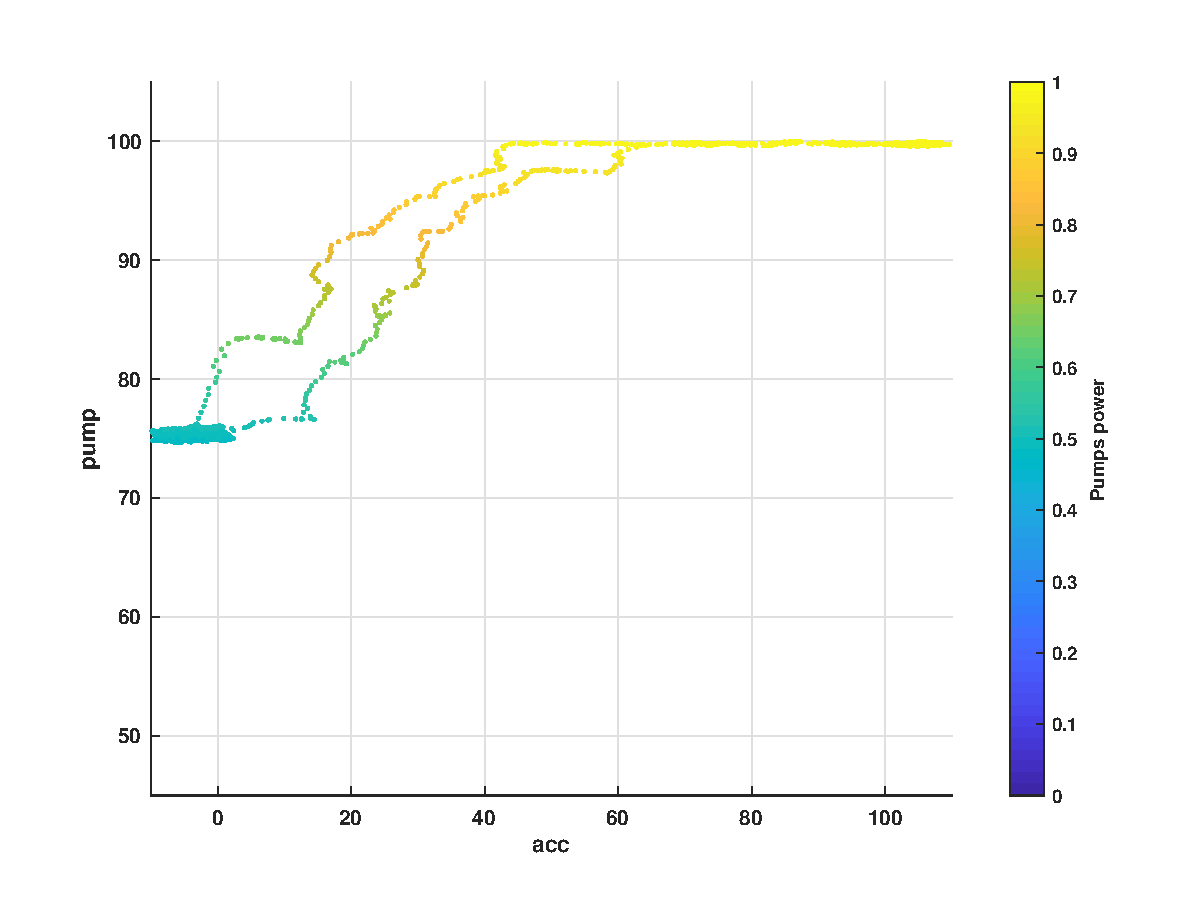
\includegraphics[height=5.8cm]{figures/pump_50_1.eps}
    \caption[Accelerator displacement against pump output]{Accelerator displacement against pump output (samples sorted based accelerator position)}
    \label{pump_50_1}
\end{figure}

I have repeated this process for all above-mentioned cases confirming that this sub-system works correctly. The figures for all the other cases can be found in appendix \ref{pumps_graphs}. To present all the results in the clear graphical way I have combined them into scatter chart plotting the accelerator against temperature values and colour mapping them by measured output \ref{Raw_pump_sum}. To show the validity of data on the right you can see the same graph with the background coloured based on a mathematical model.

\begin{figure}[h]
    \centering
        \subbottom[Measured controlling signal]{
            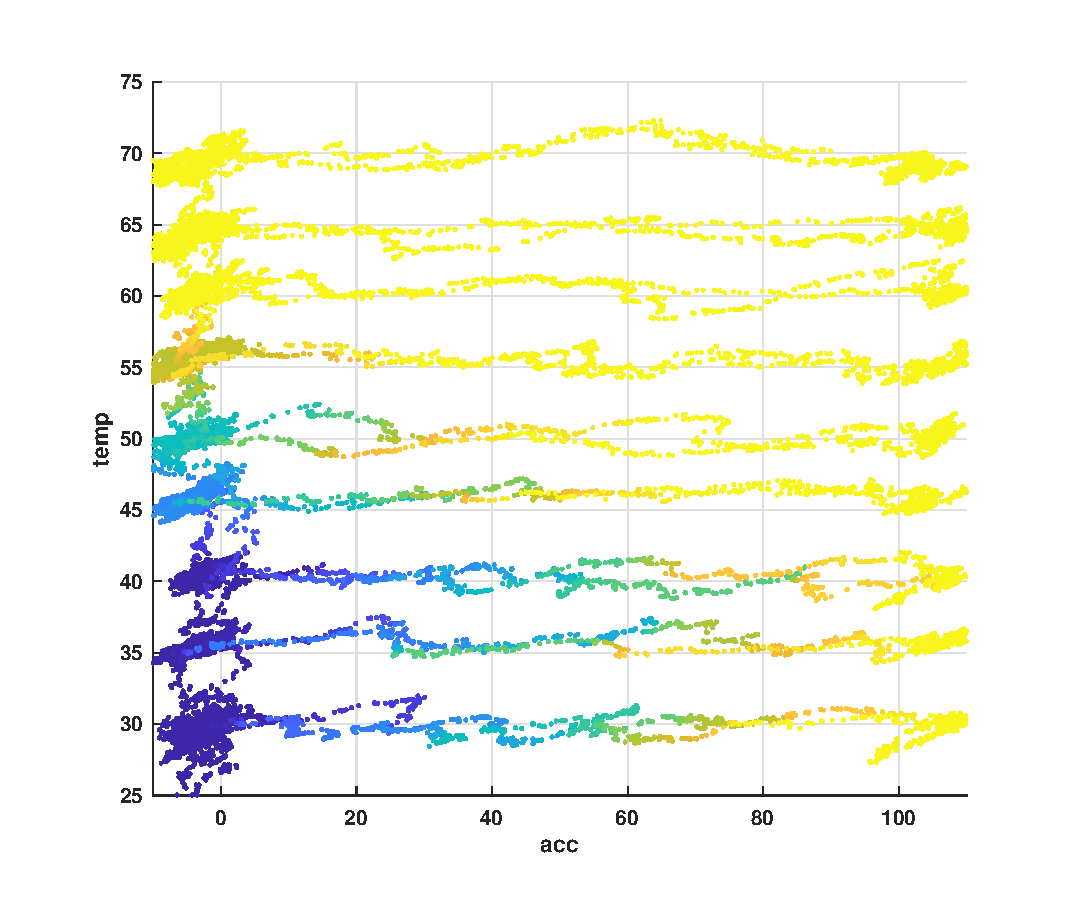
\includegraphics[height=5.8cm]{figures/Pumps_summary_raw.eps}
            \label{Raw_pump_sum}
        }
        ~
        \subbottom[With shading based on the model]{
            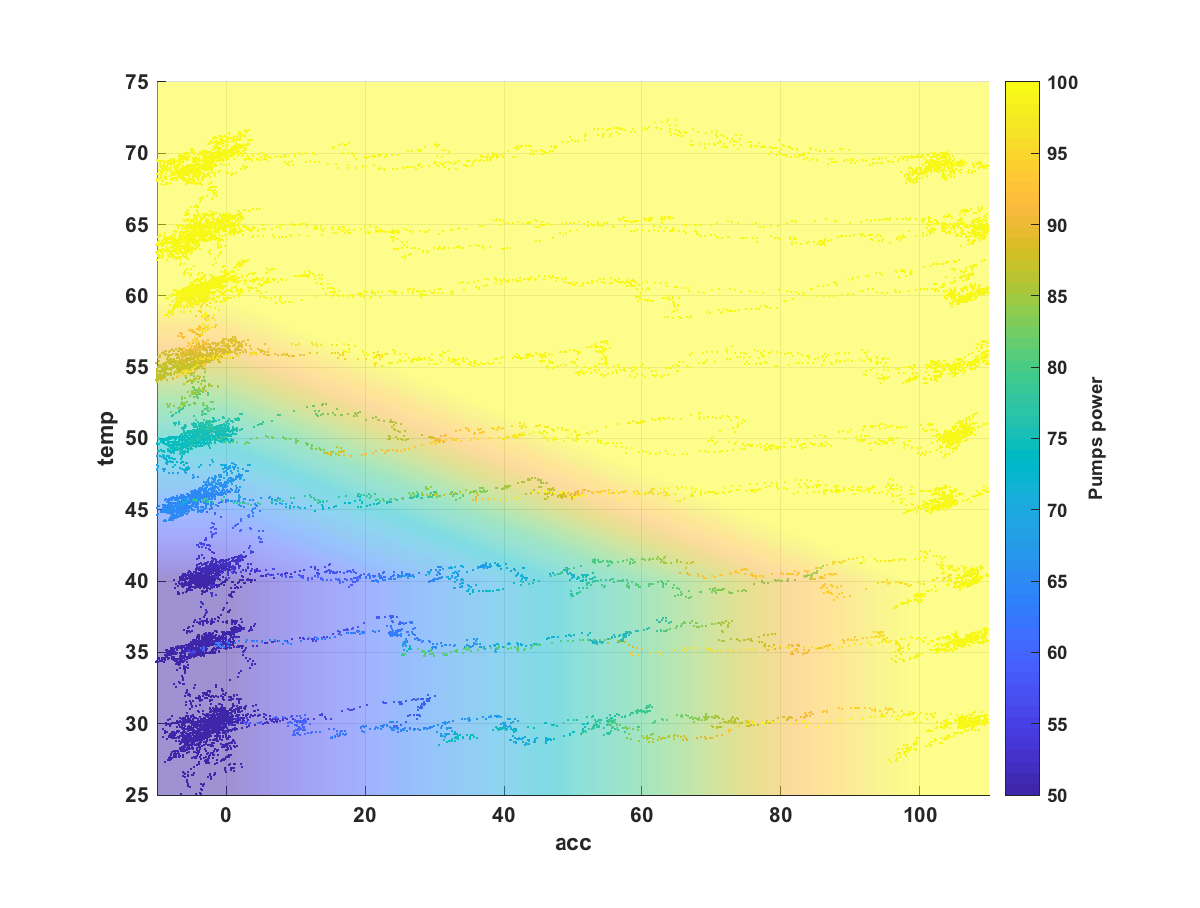
\includegraphics[height=5.8cm]{figures/Pumps_summary.eps}
            \label{Shaded_pump_sum}
        }
        \caption{Pumps control summary}
    \label{Pump_sum}
\end{figure}


\section{Regenerative Breaking}
Due to the fact that the car battery has not been finished, I have been required to make the measurements on setup powered by a laboratory amplifier. This greatly narrowed the spectrum in which I could check if the system operates correctly.

As the amplifier did not accept backward current and the car could not be driven I could not measure actual regenerative breaking. On the other hand limited current reduced dynamics of the setup and having the wheels freely spinning in the air became safely issue for high torque/speed.

To prove the validity of the programme I have measured the torque with accompanying speed for the acceleration pedal displacement from $0$ to $25\%$. As mentioned in the method section \ref{speed_mode} for first $15\%$  the control system has negative feedback loop effectively making the speed of the vehicle linearly proportional to the pedal displacement.
The pedal position has been changed by $1\%$ on each second as shown in \ref{torq_anal}. 

% \begin{wrapfigure}{!r}{0.5\textwidth}
%     \vspace{-20pt}
%     \begin{center}
%     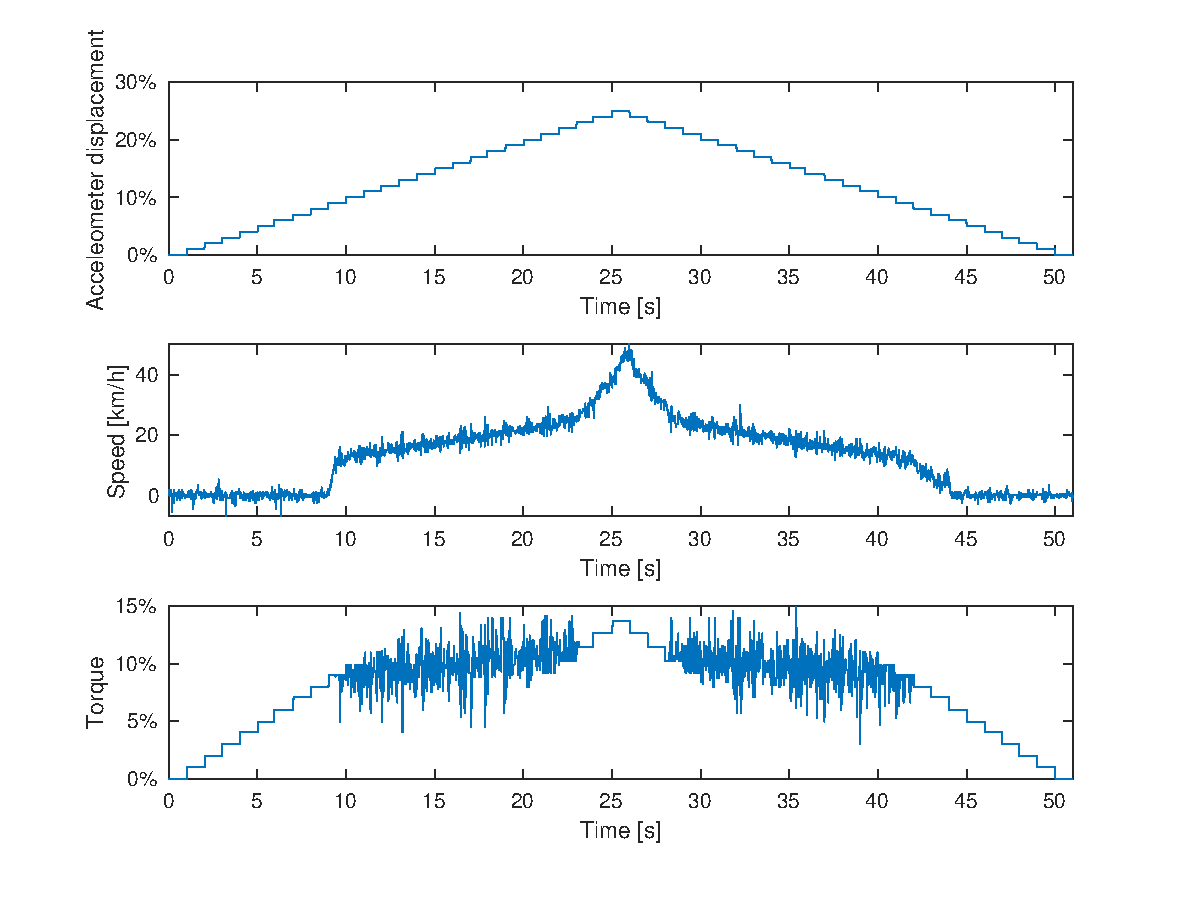
\includegraphics[width=0.48\textwidth]{figures/torq_anal}
%     \label{torq_anal}
%     \end{center}
%     \caption{Test signal for accelerator displacement}
%     \vspace{-20pt}
% \end{wrapfigure}

As expected torque output from the system was a reflection of pedal positions as long as the wheels did not spin and for speeds from $10-20 km/h$ we can observe linear dependency between pedal and speed. Then for the speeds above $20km/h$ there is simple torque control so the wheels (without load) starts to gain speed in exponential tempo.

To put in the bigger picture let me refer to the theoretical model (\ref{regen_ideal}). In the figure \ref{torq_anal} I present the measured output using the idealised model as the background. 


\begin{figure}[h]
    \centering
        \subbottom[Test signal for accelerator displacement]{
            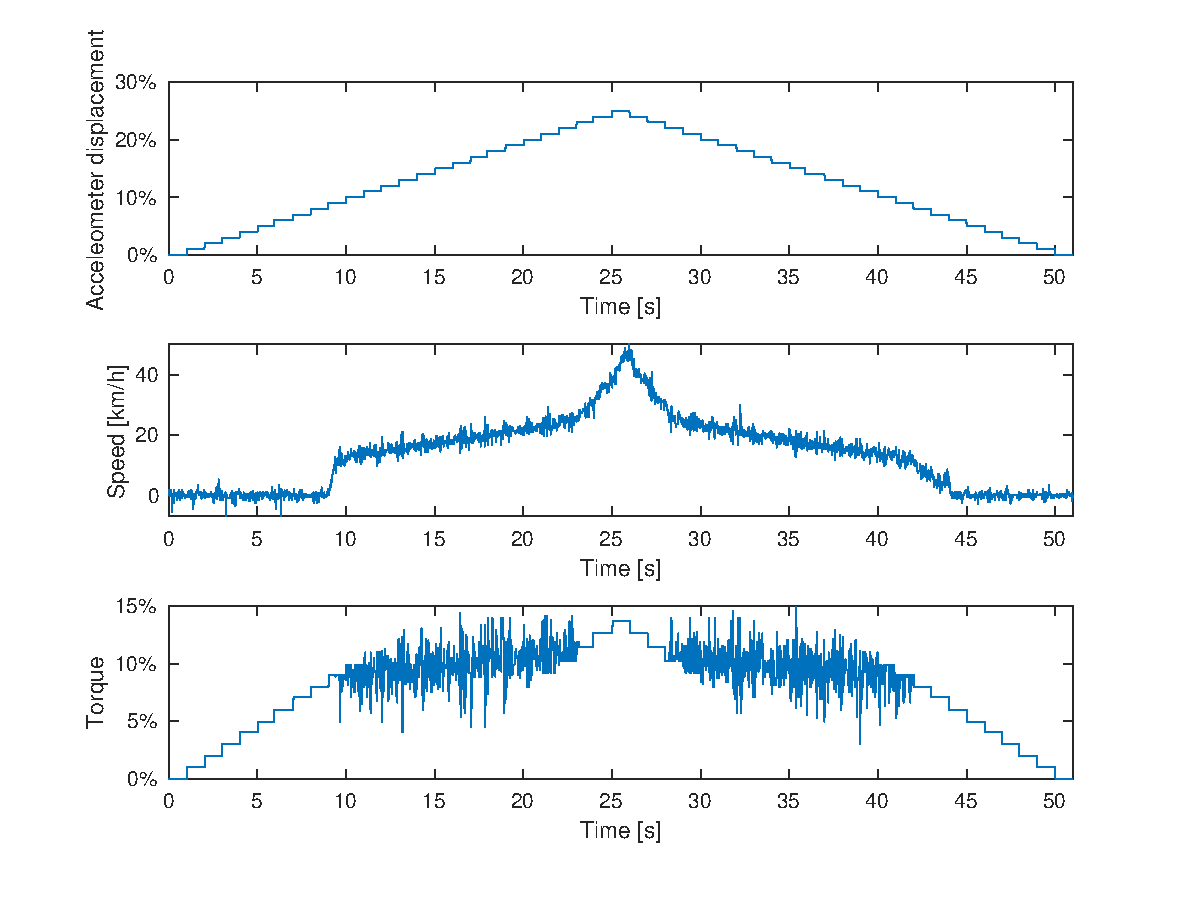
\includegraphics[width=0.46\textwidth]{figures/torq_anal}
            \label{torq_anal}
            %\caption{Test signal for accelerator displacement}
        }
        ~
        \subbottom[Measured correlation against idealised model]{
            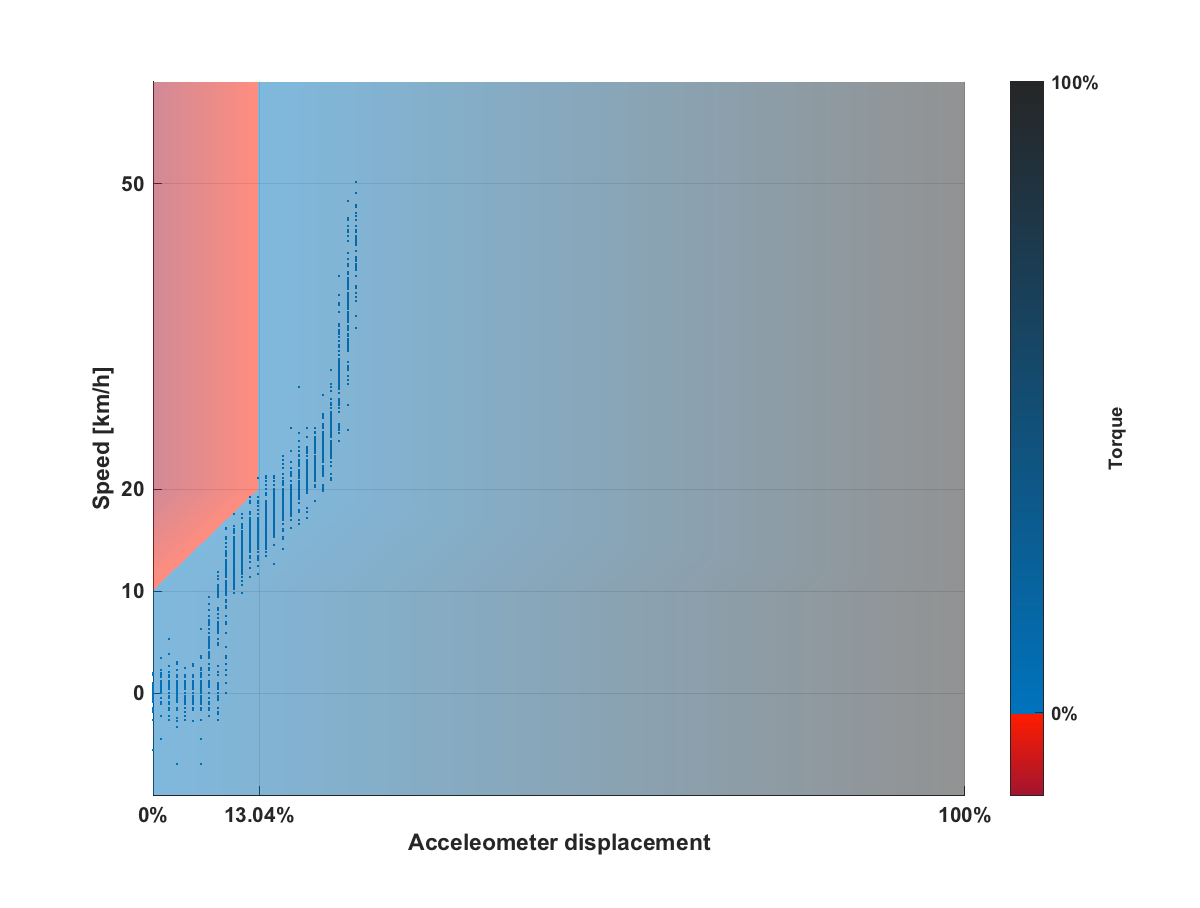
\includegraphics[width=0.46\textwidth]{figures/regen_anal.eps}
            %\caption{Measured correlation against idealised model}
            \label{regen_anal}
        }
        \caption{Torque control summary}
    \label{torq_ctl}
\end{figure}

% \begin{figure}[h]
%     \centering
%         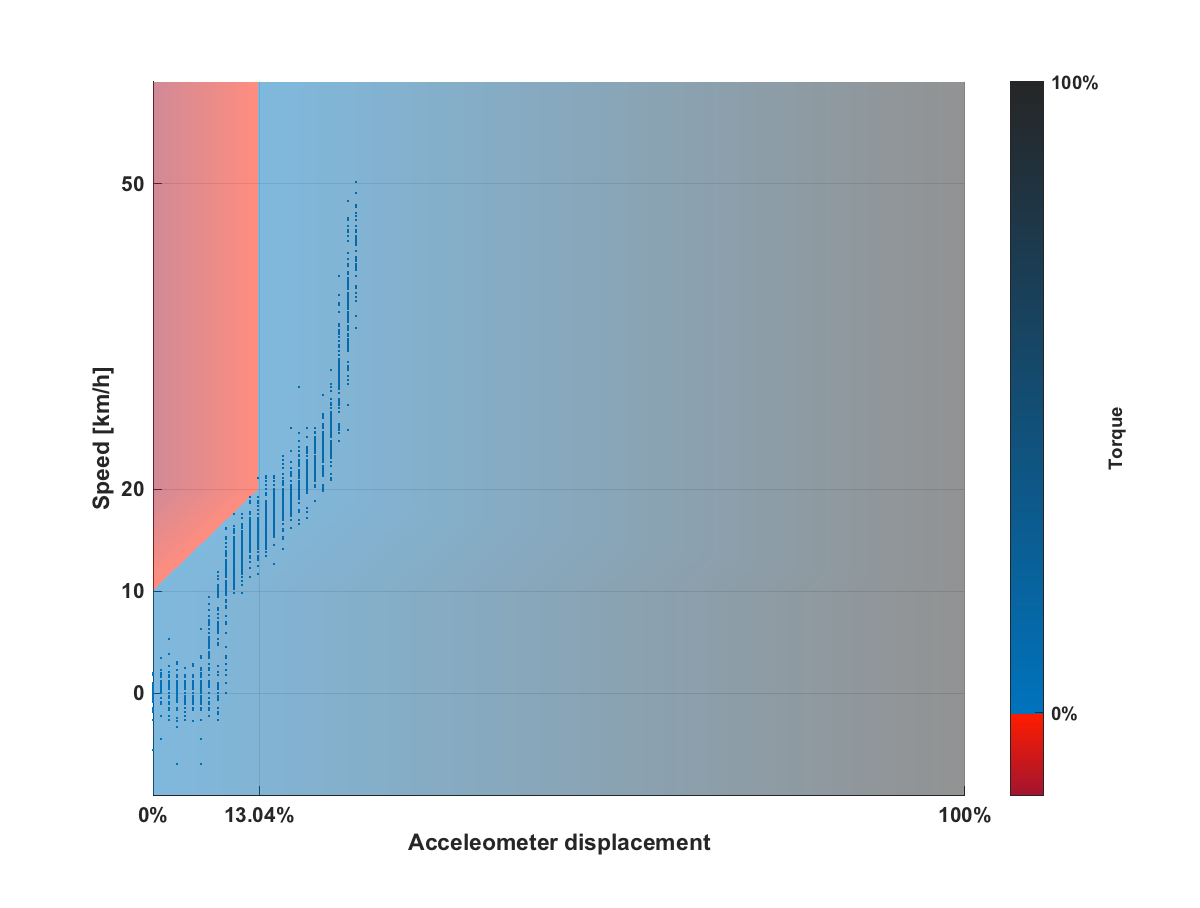
\includegraphics[height=5.8cm]{figures/regen_anal.eps}
%         \caption{Measured correlation against idealised model}
%         \label{regen_anal}
% \end{figure}

Beside above-mentioned dependencies, one can observe that there is the initial value of torque needed for a wheel to start spinning and around half a value torque to maintain its angular momentum. 

\section{Differential}
To confirm the validity of implemented model I have commit measurements where the steering wheel was rotated for each $~5\%$ displacement of acceleration pedal and where acceleration pedal was pressed fully for seemingly equally distributed 21 positions of the steering wheel in its full scale of operation. Detailed measurements results can be found in appendix \ref{diff_app}.

Meanwhile, the summarised version can be seen in figure \ref{diff_sum}.

\begin{figure}[h]
    \centering
        \subbottom[]{
            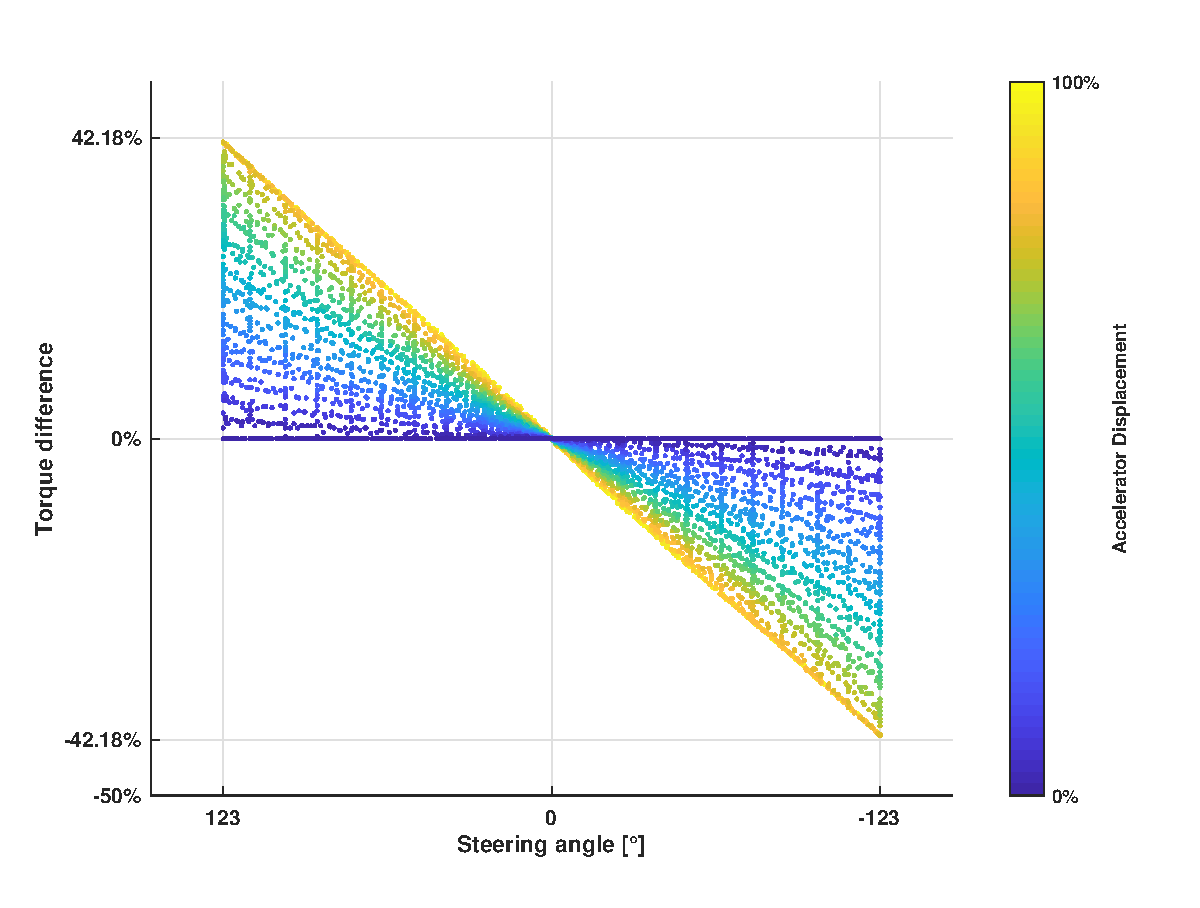
\includegraphics[width=0.46\textwidth]{figures/ste_torq.eps}
            \label{}
            %\caption{Test signal for accelerator displacement}
        }
        ~
        \subbottom[]{
            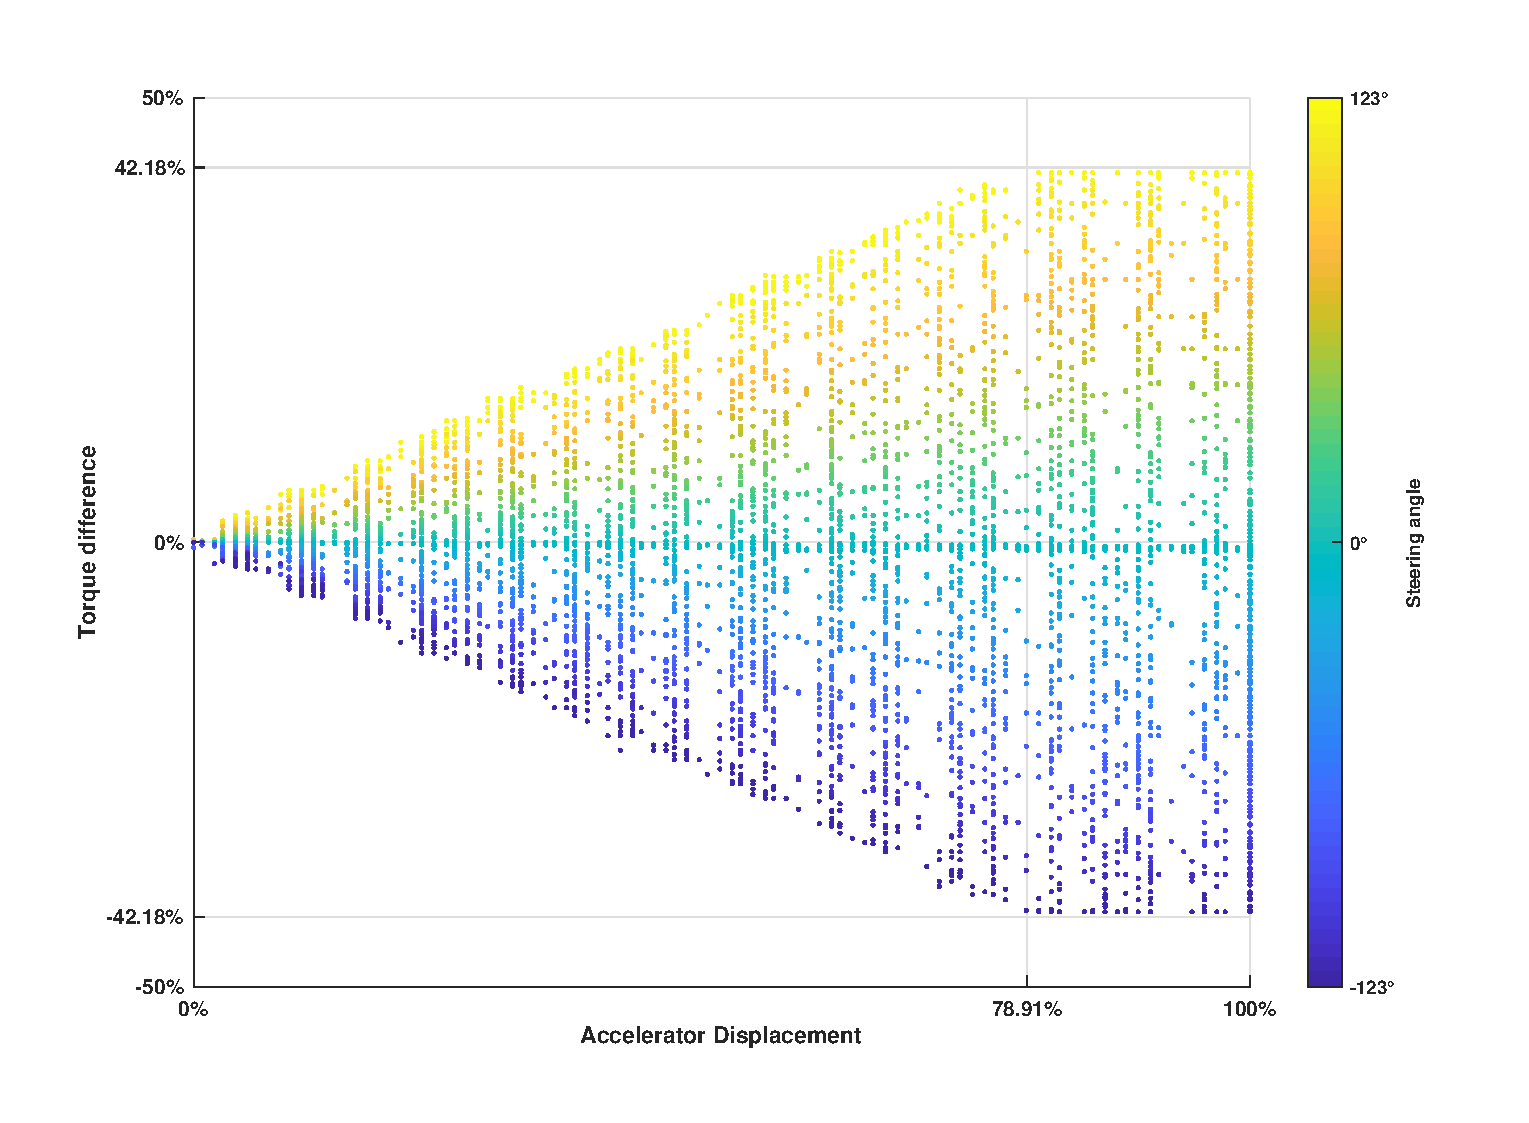
\includegraphics[width=0.46\textwidth]{figures/acc_torq.eps}
            %\caption{Measured correlation against idealised model}
            \label{diff_sum_b}
        }
        \caption{Relation between acceleration pedal displacement, steering wheel angle and normalised torque difference}
    \label{diff_sum}
\end{figure}

As one can notice in \ref{diff_sum_b} motor torque difference is linearly proportional to acceleration pedal and steering wheel displacement. This relation is clearly maintained for first $\~80\%$ of pedal travel and it saturates on torque difference equal about $42\%$ in rest of the scale. It is the desired behaviour of this control. To explain all the values let me refer to equations \ref{diff_eq} and \ref{diff_eq_w} from the theory section.

In the vehicle, I have been working on has the maximum steering angle of 36°, wheelbase 1740mm and track equal to 1270mm. Taking these values together into mentioned equations results in wheel disproportion: 

\begin{equation*}
    \alpha_{inner} = 0.7349 ~~~~~
    \alpha_{outer} = 1.2651
\end{equation*}

From this point target torque is calculated simply by multiplication with the percent of pedal displacement and maximum torque. What is reflected in measurements for first $80\%$ of pedal travel. 
Behaviour in remaining $20\%$ is a result of limited power and accompanying safety feature described in \ref{diff_meth}. To make differential functional while using near full available power desired torque is scaled down to the maximum torque per wheel is never exceed (equation \ref{diff_saf}).
The functionality is simply active if only: \begin{equation*}
    \alpha_{outer} * d_{acc}>1
\end{equation*} 
Where:
\begin{description}
    \item[$d_{acc}$] acceleration pedal displacement
\end{description}

\begin{wrapfigure}{!r}{0.5\textwidth}
    \vspace{-20pt}
    \begin{center}
        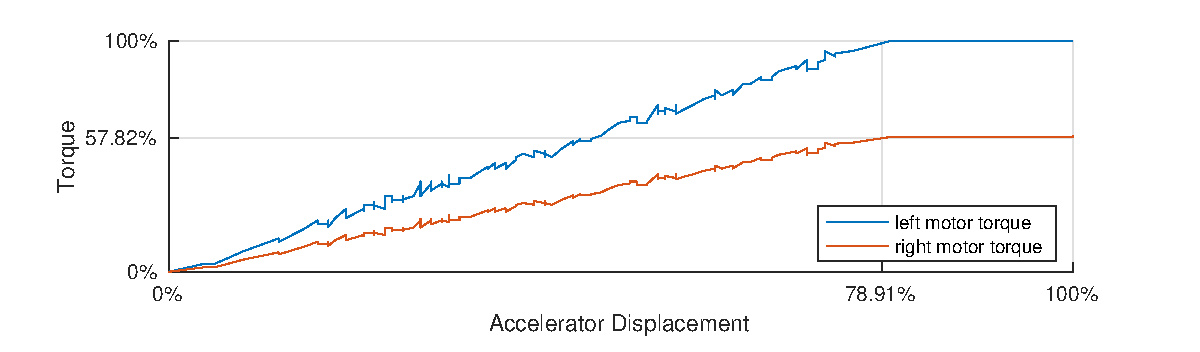
\includegraphics[width=0.46\textwidth]{figures/diff_123}
        \label{diff_123}
        \caption{Motors torque compassion for steering wheel rotated 124° (maximum steering angle) left}
    \end{center}
    \vspace{-20pt}
\end{wrapfigure}
So taking into consideration maximum steering angle it becomes active for $d_{acc} \approx 78.91\%$ which can been seen in figure \ref{diff_sum_b}.

To further confirm this safety functionality figure \ref{diff_123} consist only of samples for maximum steering angle independently showing the torque of two wheels. The outer wheel saturates on maximum torque where the inner one maintains proportion needed for differential steering.







\section{System performance}
As mentioned due to the malfunctioning motor controller the system performance was limited. However, as I am going to show in the next figures implemented workaround performs considerably well and is not a bottleneck in a current state.

Place where the timing is the most important is in between receiving of pedal/steering wheel status and sending torque control signal to drives.
\begin{figure}[h]
    \centering
            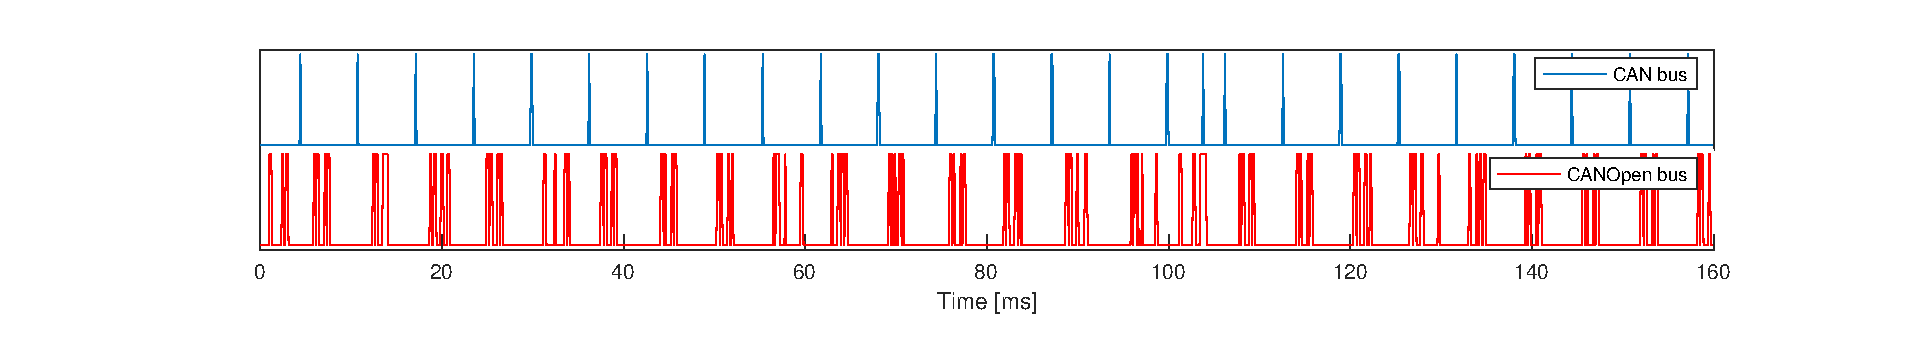
\includegraphics[width=0.8\textwidth]{figures/perf_rep.eps}
            \label{perf_over}
            \caption{CAN and CANOpen timing overview}
\end{figure}

As shown in the figure \ref{perf_over} there are messages on the CAN bus which appears within a constant interval of about $6,8 ms$. Each of these messages contains break, accelerator and steering wheel position and the timing is close to one estimated in method chapter (\ref{pedal_ideal_time}) of $5,2 ms$.

Each sensors position message is closely followed by four messages on CANOpen bus which are responsible for accordingly changing target torque values in motor controllers. 
\begin{figure}[h]
    \centering
            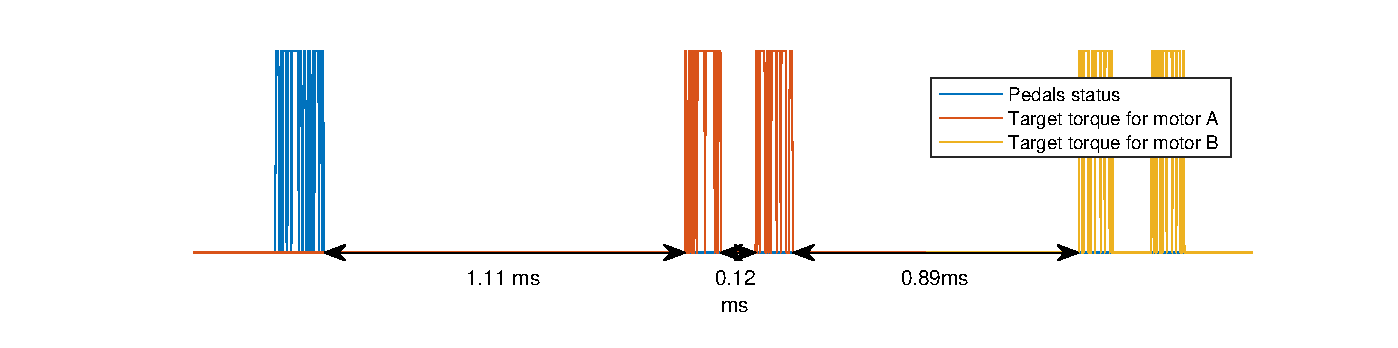
\includegraphics[width=0.8\textwidth]{figures/perf.eps}
            \label{perf}
            \caption{Control torque loop timing}
\end{figure}
As shown in figure \ref{perf} after receiving it takes just $~1.11 ms$ to first respond and second respond is sent in $~0.89 ms$ after. As in the code, two calls to LabVIEW closed library responsible for CANOpen communication are issued one after another, it suggests that in both cases about $0.89 ms$ is taken to just send a message. Therefore I am convinced that CAN receive code, interrupt issue it service and torque calculations take only about $0.22 ms$ of total time.
%!TEX root = ../Thesis.tex

% 5. Discussion
% In many thesis the discussion is the most important section. Make sure that you allocate enough time and space for a good discussion. This is your opportunity to show that you have understood the significance of your findings and that you are capable of applying theory in an independent manner.

% The discussion will consist of argumentation. In other words, you investigate a phenomenon from several different perspectives. To discuss means to question your findings, and to consider different interpretations. Here are a few examples of formulations that signal argumentation:

% On the one hand … and on the other …
% However …
% … it could also be argued that …
% … another possible explanation may be …
%!TEX root = ../Thesis.tex

% 6. Conclusion – or summing up?

% The final section of your thesis may take one of several different forms. Some theses need a conclusion, while for others a summing up will be appropriate. The decisive factor will be the nature of your thesis statement and/or research question.

% Open research questions cannot always be answered, but if a definite answer is possible, you must provide a conclusion. The conclusion should answer your research question(s). Remember that a negative conclusion is also valid.

% A summing up should repeat the most important issues raised in your thesis (particularly in the discussion), although preferably stated in a (slightly) different way. For example, you could frame the issues within a wider context.

% Placing your thesis in perspective

% In the final section you should place your work in a wider, academic perspective and determine any unresolved questions. During the work, you may have encountered new research questions and interesting literature which could have been followed up. At this point, you may point out these possible developments, while making it clear for the reader that they were beyond the framework of your current project.

% Briefly discuss your results through a different perspective. This will allow you to see aspects that were not apparent to you at the project preparation stage
% Highlight alternative research questions that you have found in the source materials used in the project
% Show how others have placed the subject area in a wider context
% If others have drawn different conclusions from yours, this will provide you with ideas of new ways to view the research question
% Describe any unanswered aspects of your project
% Specify potential follow up and new projects
% A thesis should “bite itself in the tail”

% There should be a strong connection between your conclusion and your introduction. All the themes and issues that you raised in your introduction must be referred to again in one way or another. If you find out at this stage that your thesis has not tackled an issue that you raised in the introduction, you should go back to the introduction and delete the reference to that issue. An elegant way to structure the text is to use the same textual figure or case in the beginning as well as in the end. When the figure returns in the final section, it will have taken on a new and richer meaning through the insights you have encountered, created in the process of writing.

\chapter{Conclusion}\label{total:chapters}


The circumstances during the work on my thesis indirectly but forced me to work on wide spectrum of tasks. Although interesting, it did not allow me to make these studies more in depth on any particular part. 
I believe, I have had 

Narra strong base so the future students working on the project will ow able to isolate each small subsystem, work on them independently and bring a great amount of improvements.ing the scobuild pe of youber thesis can be time-consuming. Paradoxically, the more you limit the scope, the more interesting it becomes. This is because a narrower scope lets you clarify the problem and study it at greater depth, whereas very broad research questions only allow a superficial treatment. 
\chapter{Scratch}



% \blinddocument

\appendix
\Chapter{}{Pump control measurements}\label{pumps_graphs}
\begin{figure}[h]
    \centering
        \subbottom[Temperature set to 30\textdegree C and varying accelerator displacement]{
            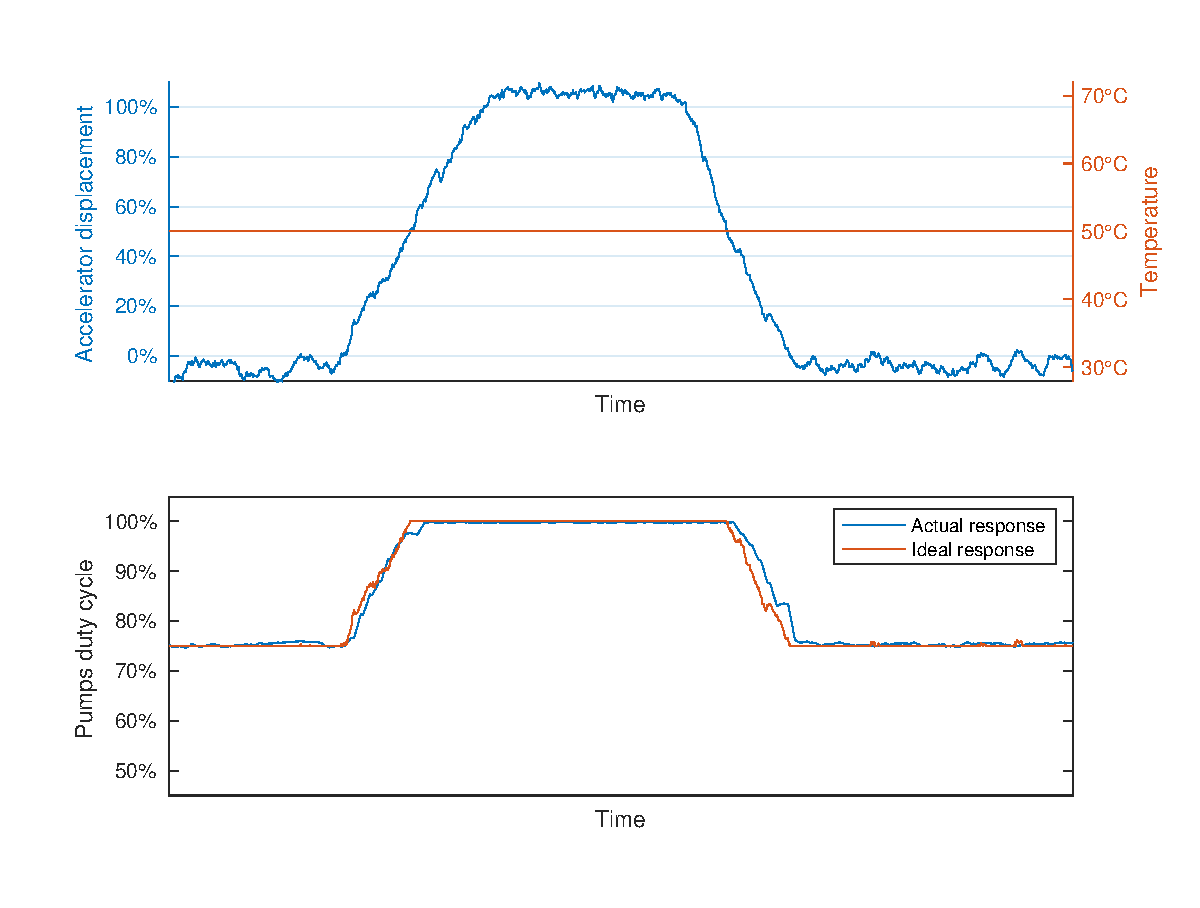
\includegraphics[height=5cm]{figures/pump_50.eps}
            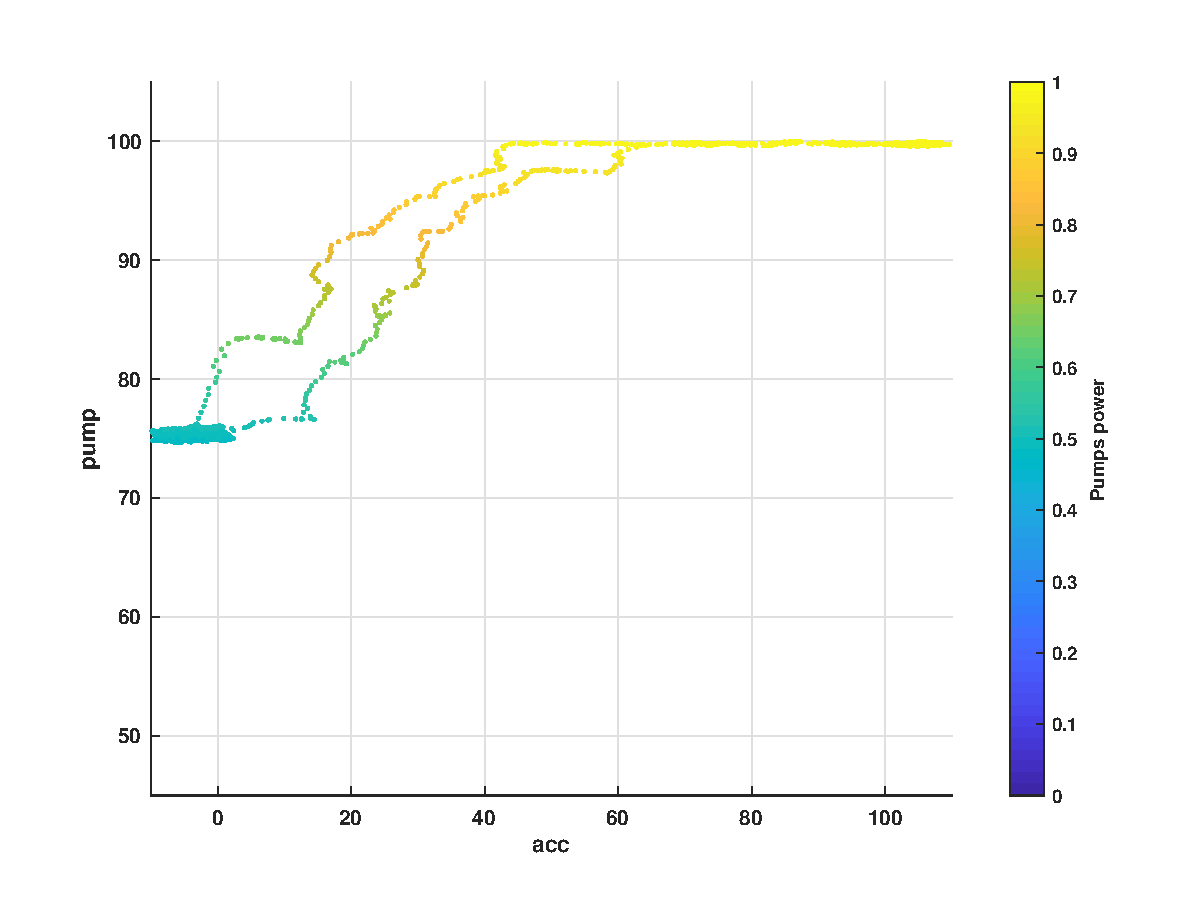
\includegraphics[height=5cm]{figures/pump_50_1.eps}
        }
        ~
        \subbottom[Temperature set to 35\textdegree C and varying accelerator displacement]{
            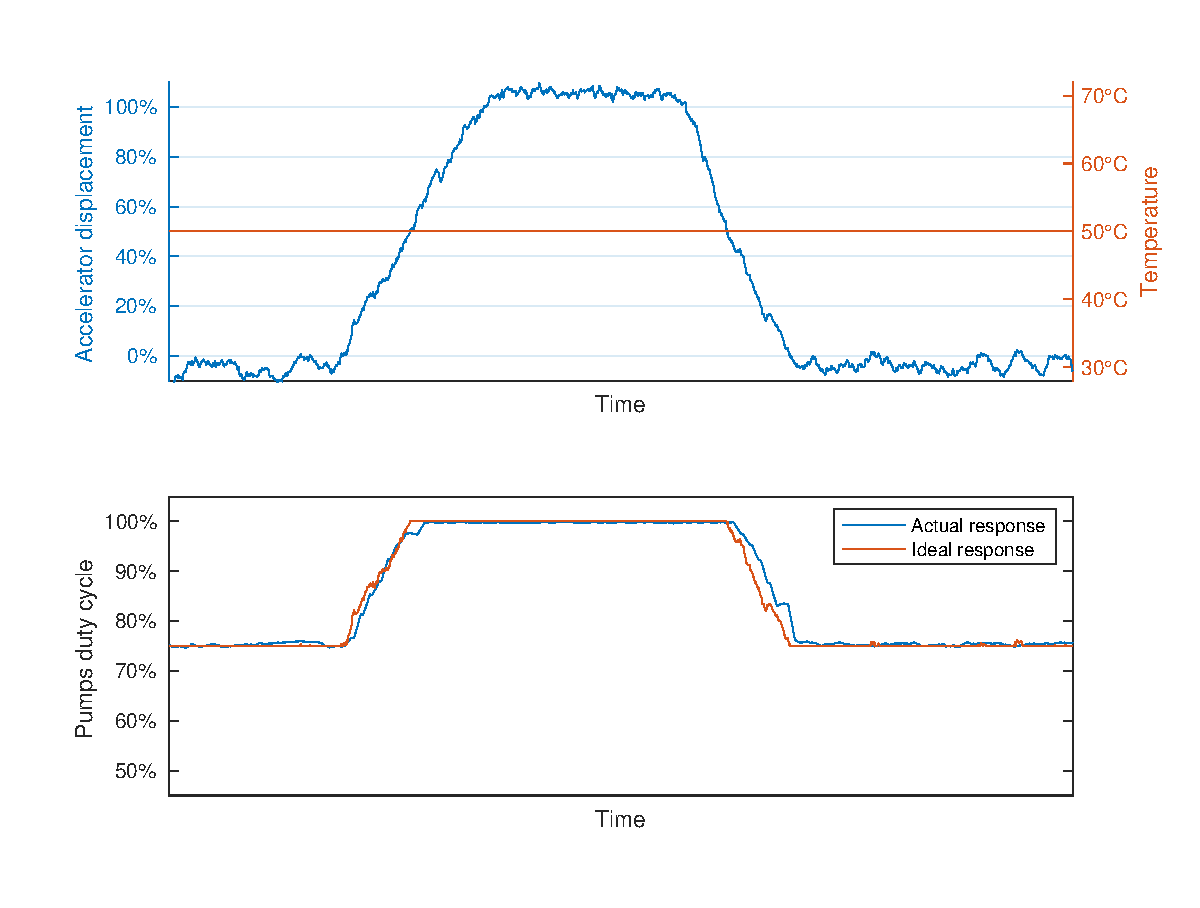
\includegraphics[height=5cm]{figures/pump_50.eps}
            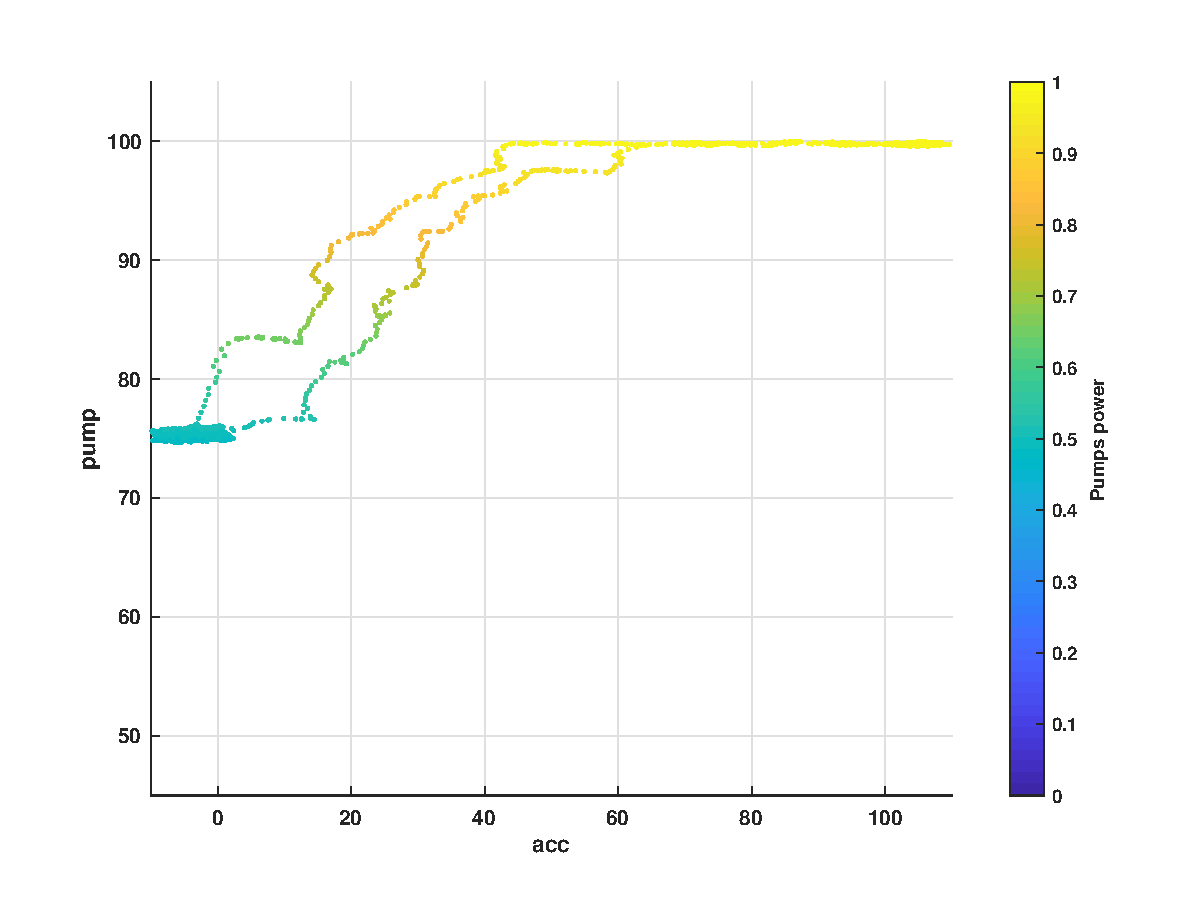
\includegraphics[height=5cm]{figures/pump_50_1.eps}
        }
        ~
        \subbottom[Temperature set to 40\textdegree C and varying accelerator displacement]{
            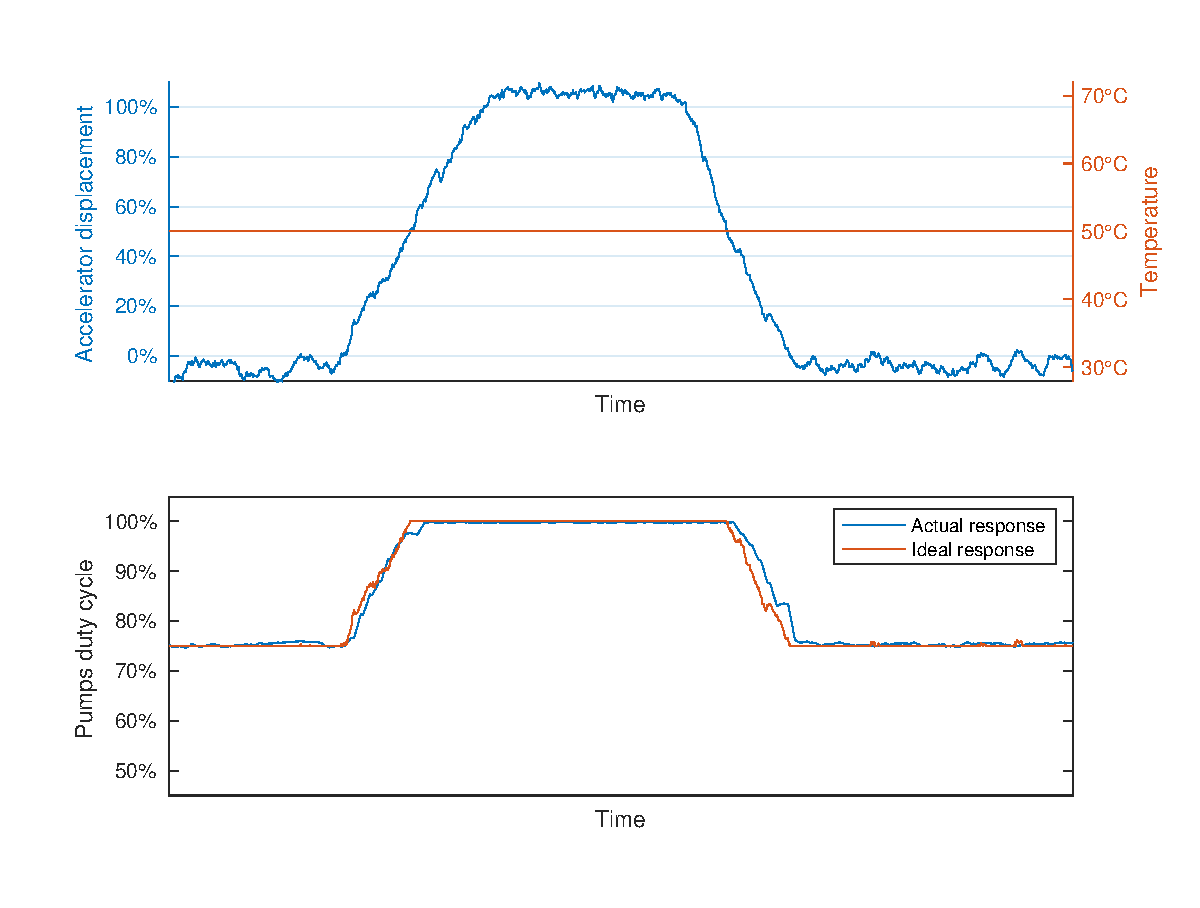
\includegraphics[height=5cm]{figures/pump_50.eps}
            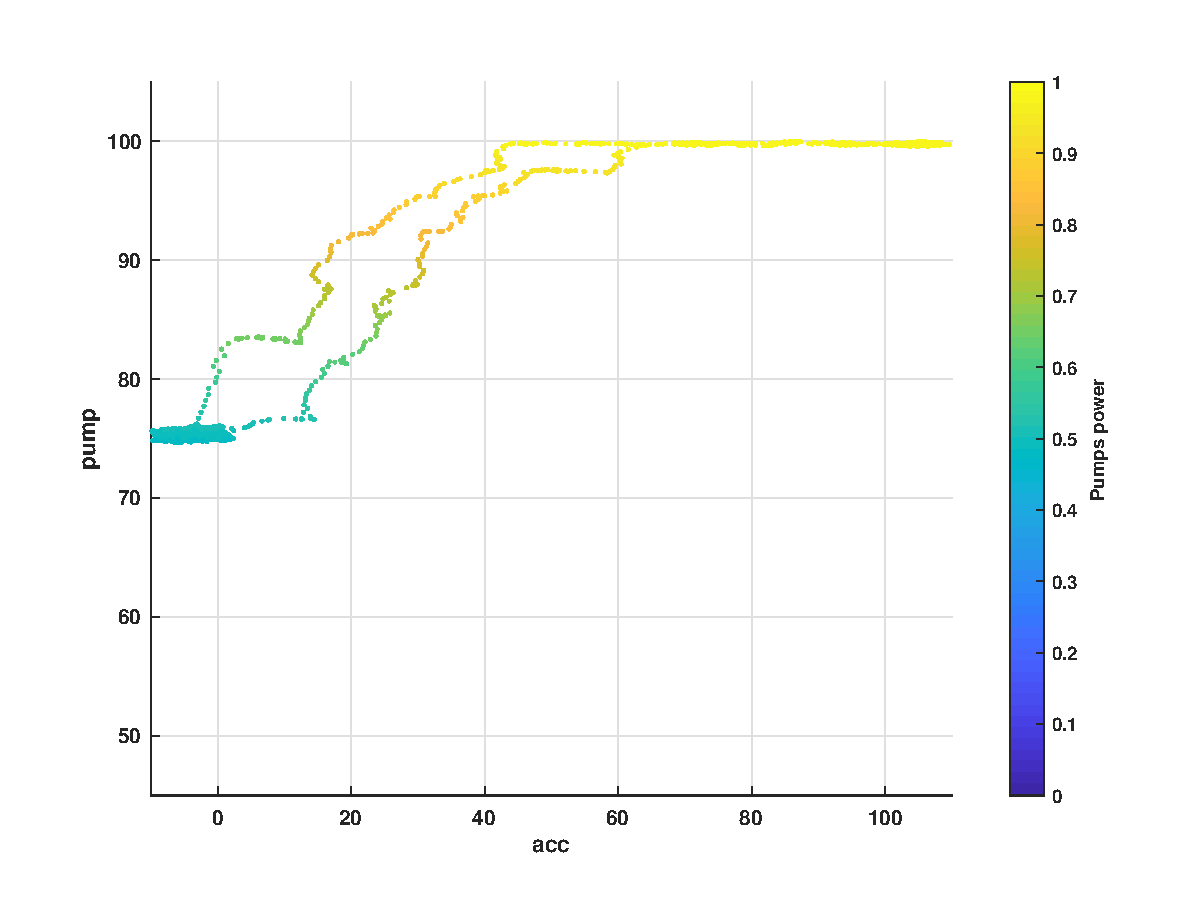
\includegraphics[height=5cm]{figures/pump_50_1.eps}
        }
        % \caption{}
\end{figure}
\begin{figure}[h]
    \centering
        \subbottom[Temperature set to 45\textdegree C and varying accelerator displacement]{
            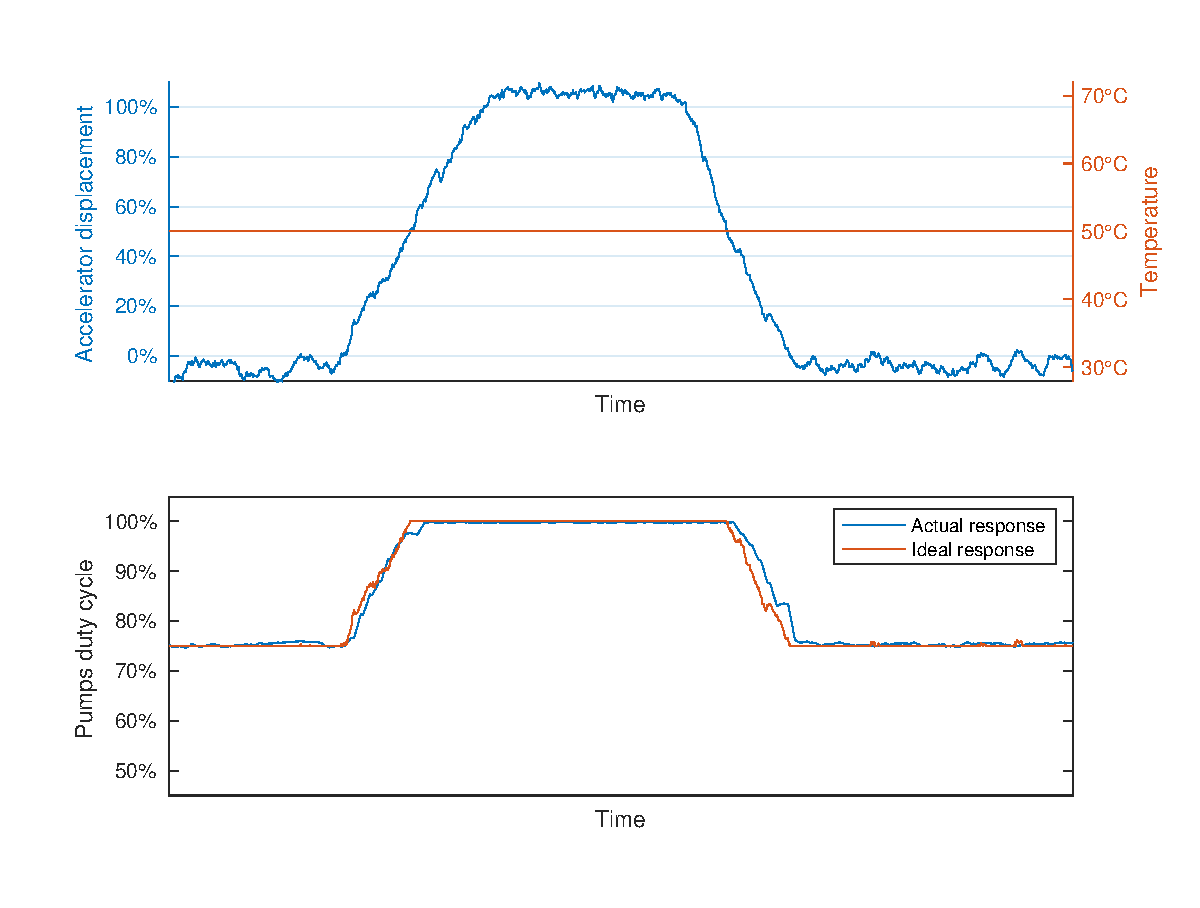
\includegraphics[height=5cm]{figures/pump_50.eps}
            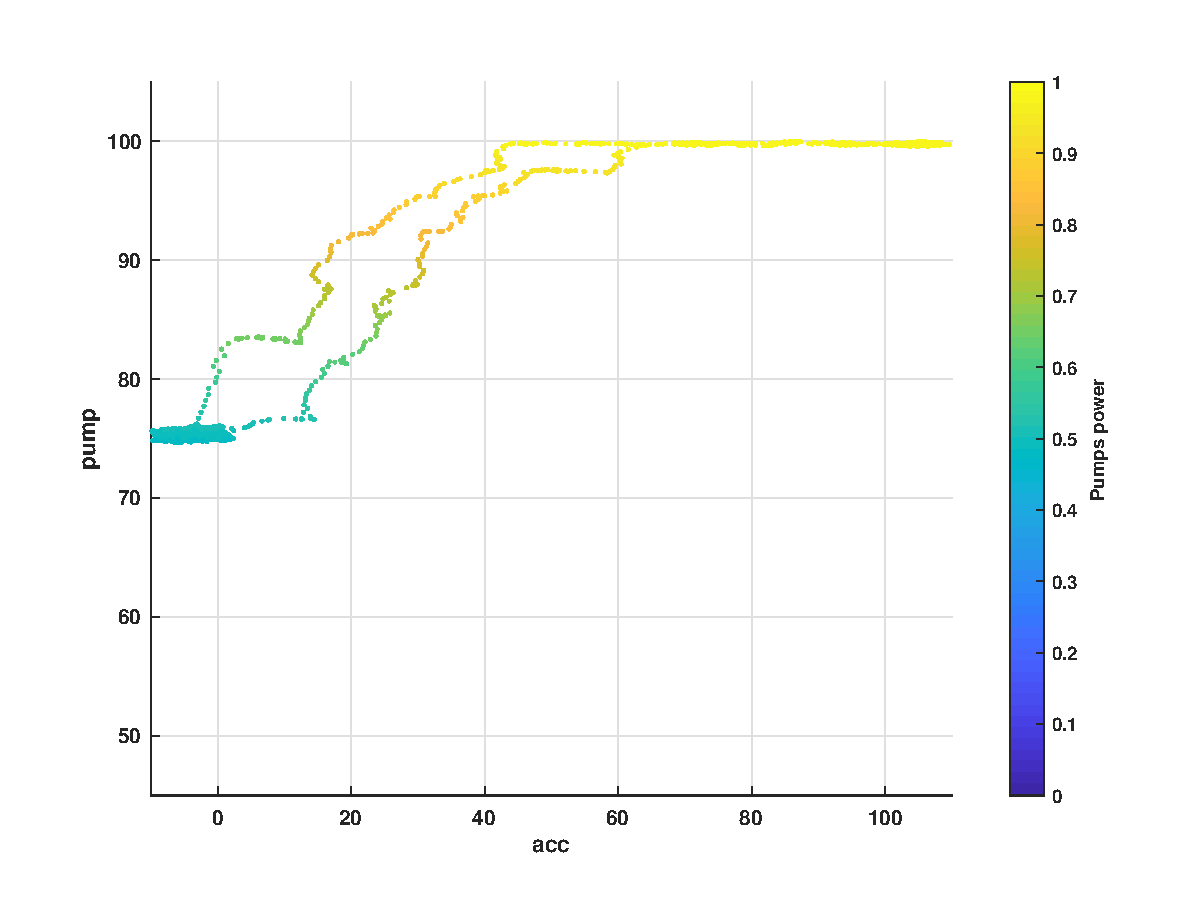
\includegraphics[height=5cm]{figures/pump_50_1.eps}
        }
        ~
        \subbottom[Temperature set to 50\textdegree C and varying accelerator displacement]{
            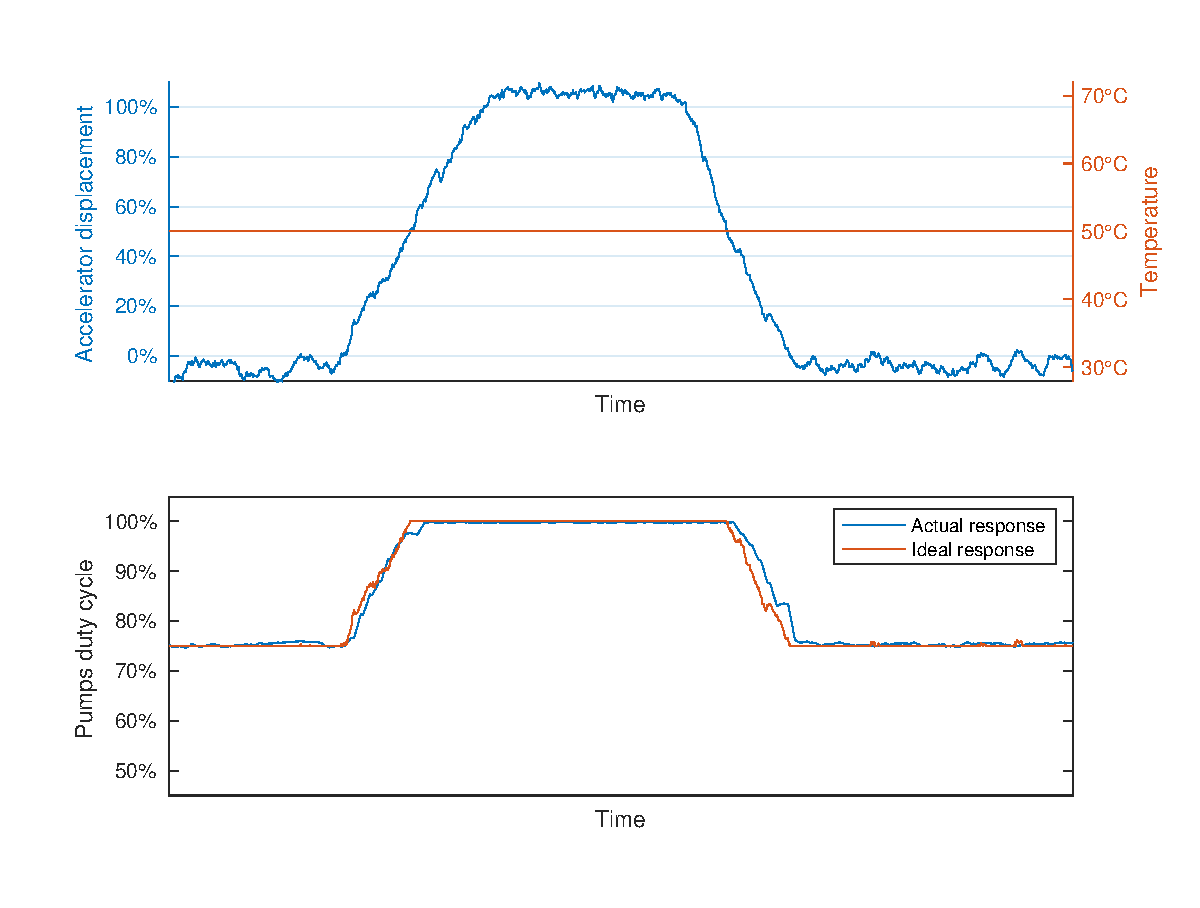
\includegraphics[height=5cm]{figures/pump_50.eps}
            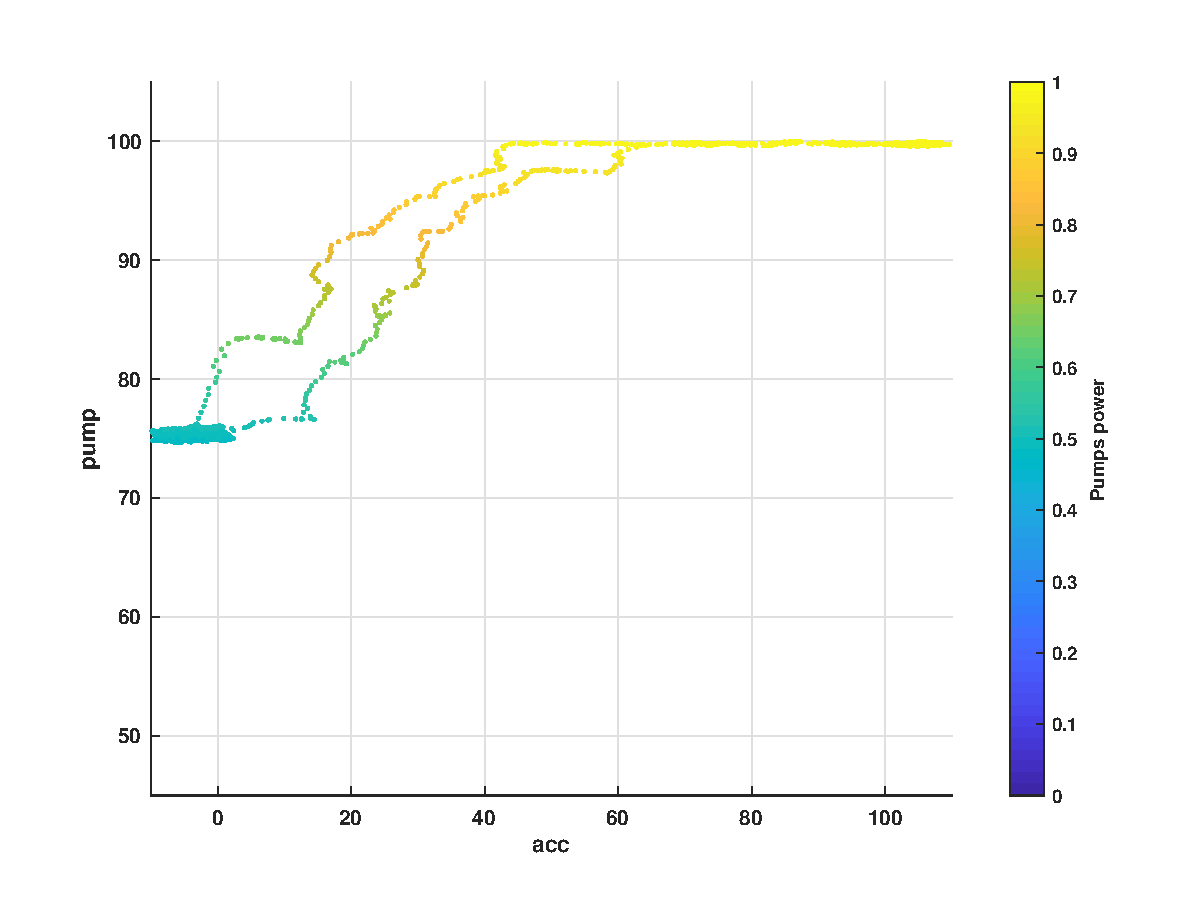
\includegraphics[height=5cm]{figures/pump_50_1.eps}
        }
        ~
        \subbottom[Temperature set to 55\textdegree C and varying accelerator displacement]{
            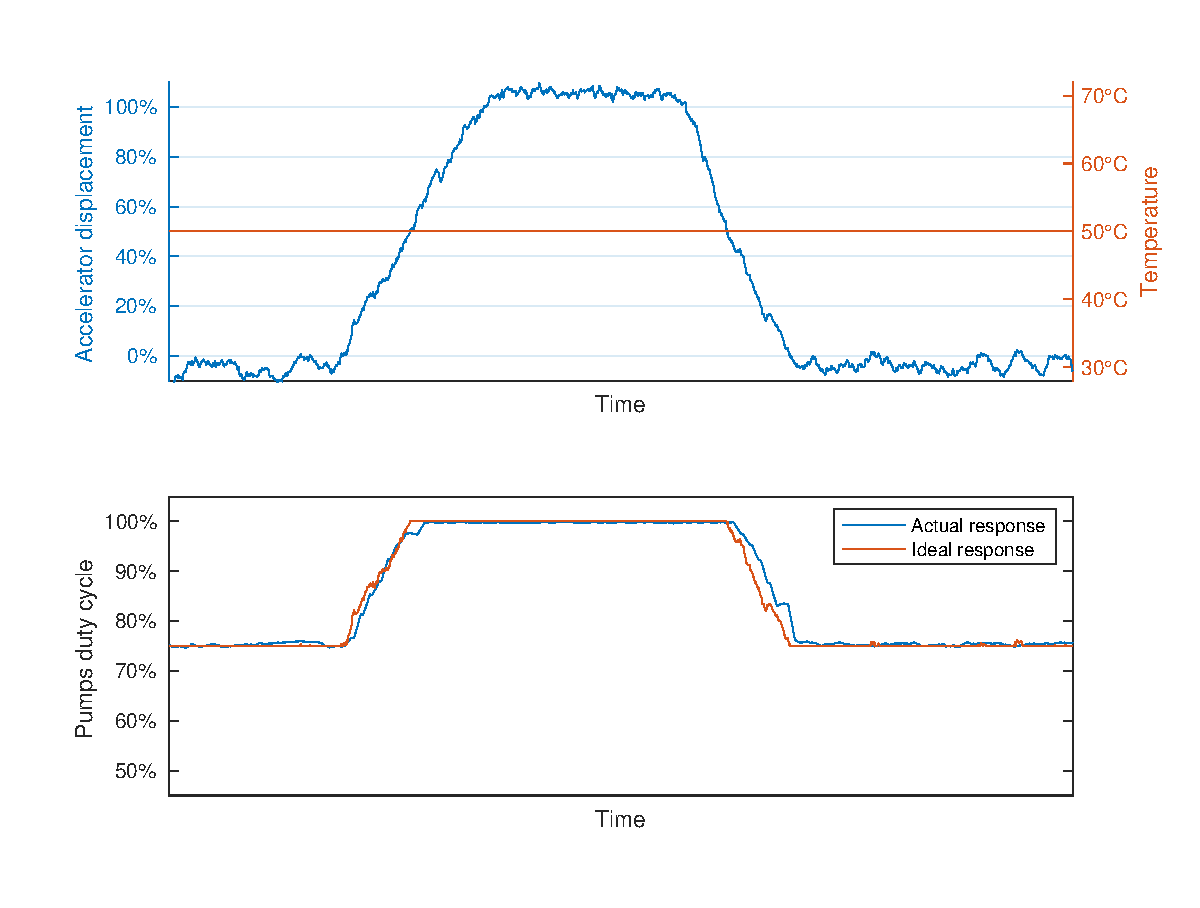
\includegraphics[height=5cm]{figures/pump_50.eps}
            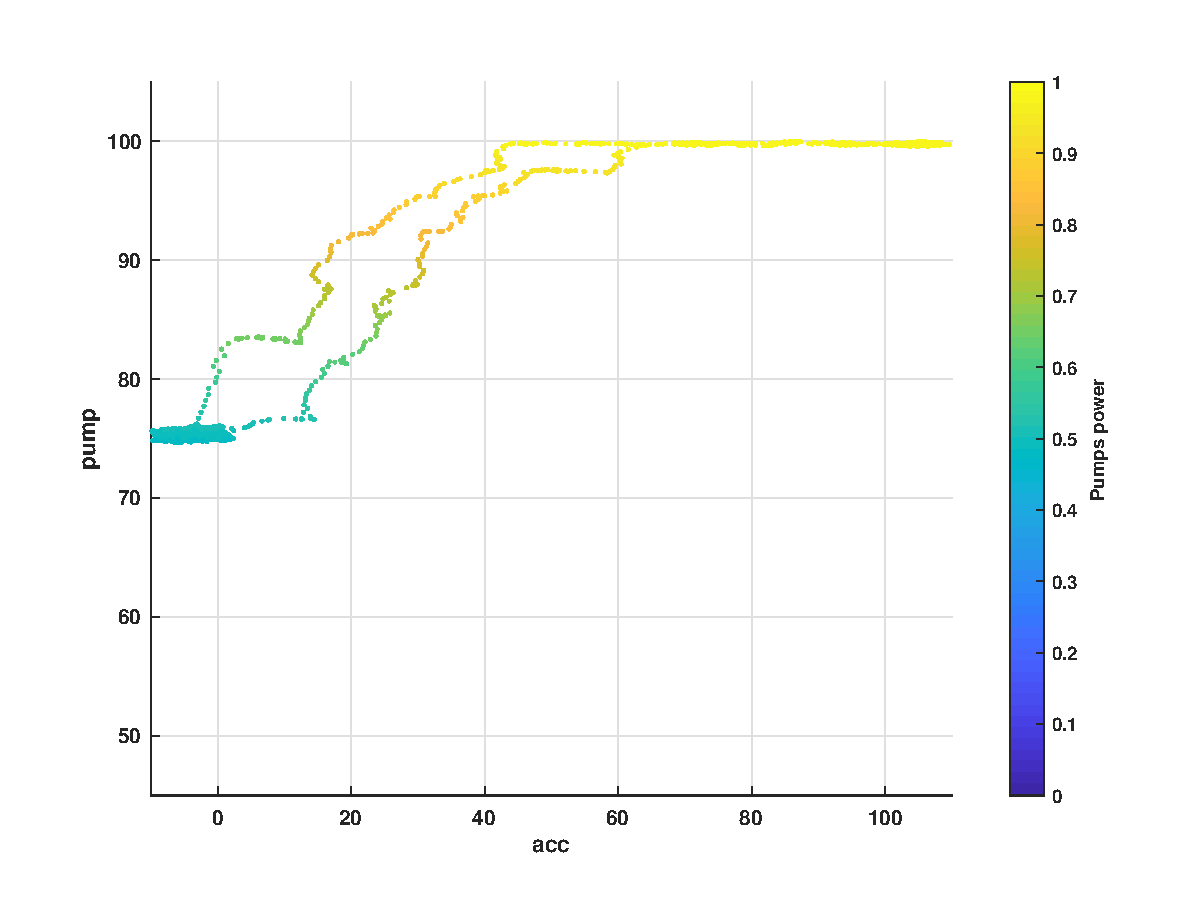
\includegraphics[height=5cm]{figures/pump_50_1.eps}
        }
        ~
        \subbottom[Temperature set to 60\textdegree C and varying accelerator displacement]{
            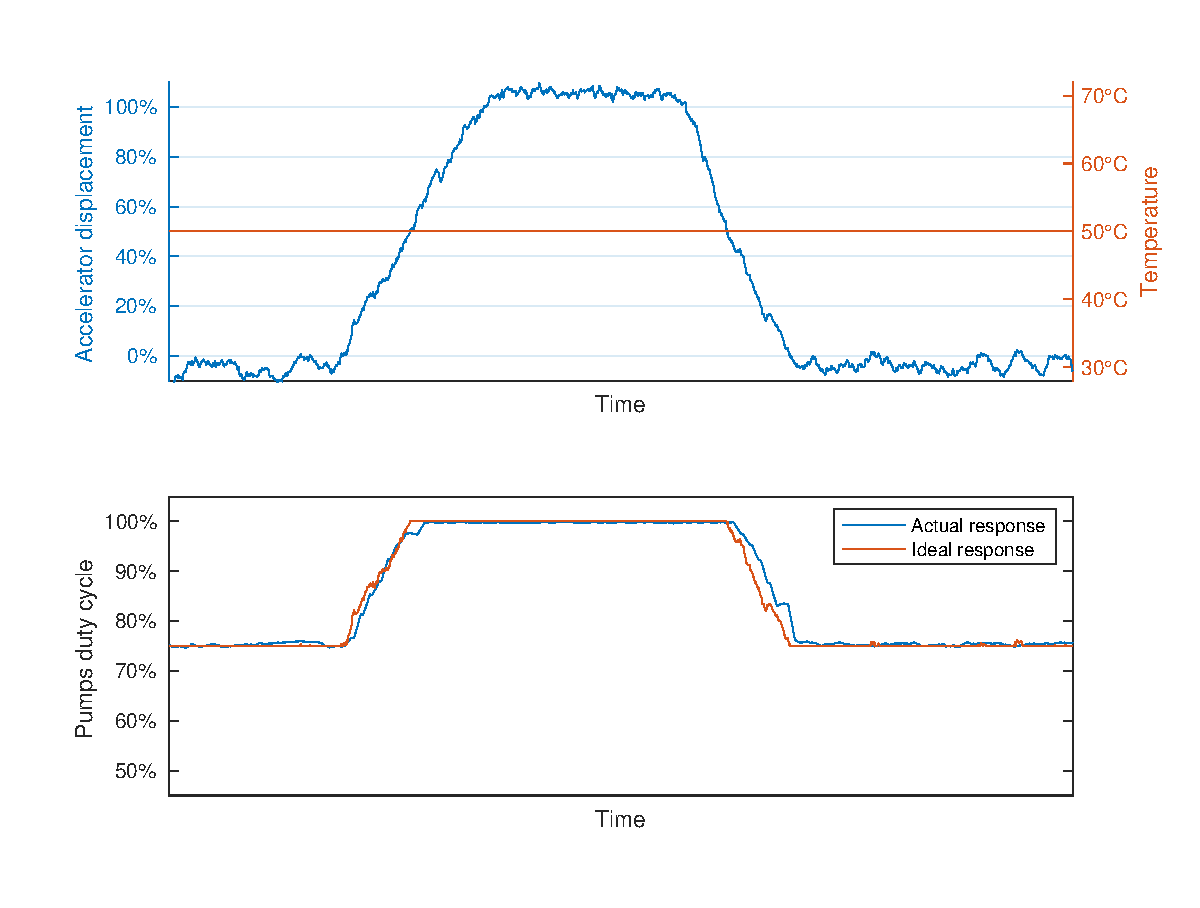
\includegraphics[height=5cm]{figures/pump_50.eps}
            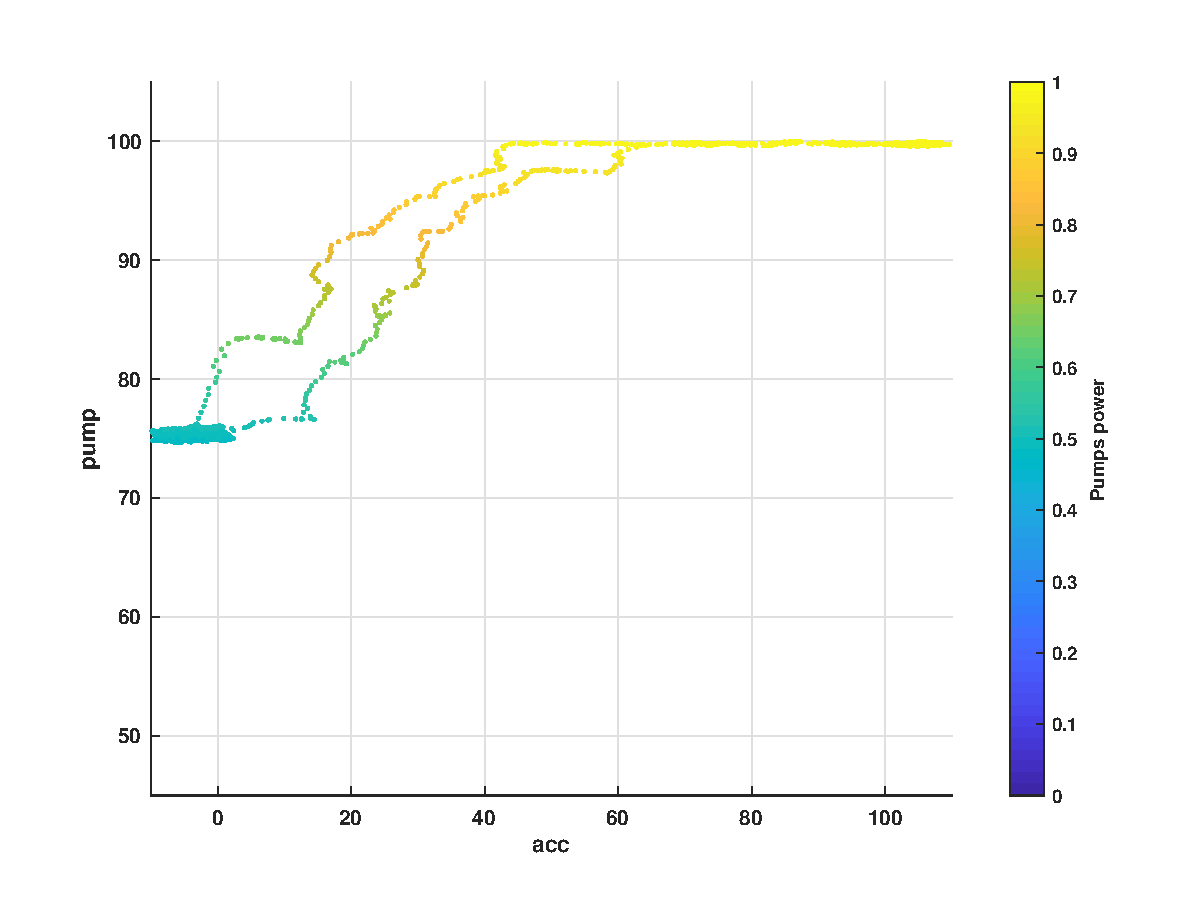
\includegraphics[height=5cm]{figures/pump_50_1.eps}
        }
        % \caption{}
\end{figure}
\begin{figure}[h]
    \centering
        \subbottom[Temperature set to 65\textdegree C and varying accelerator displacement]{
            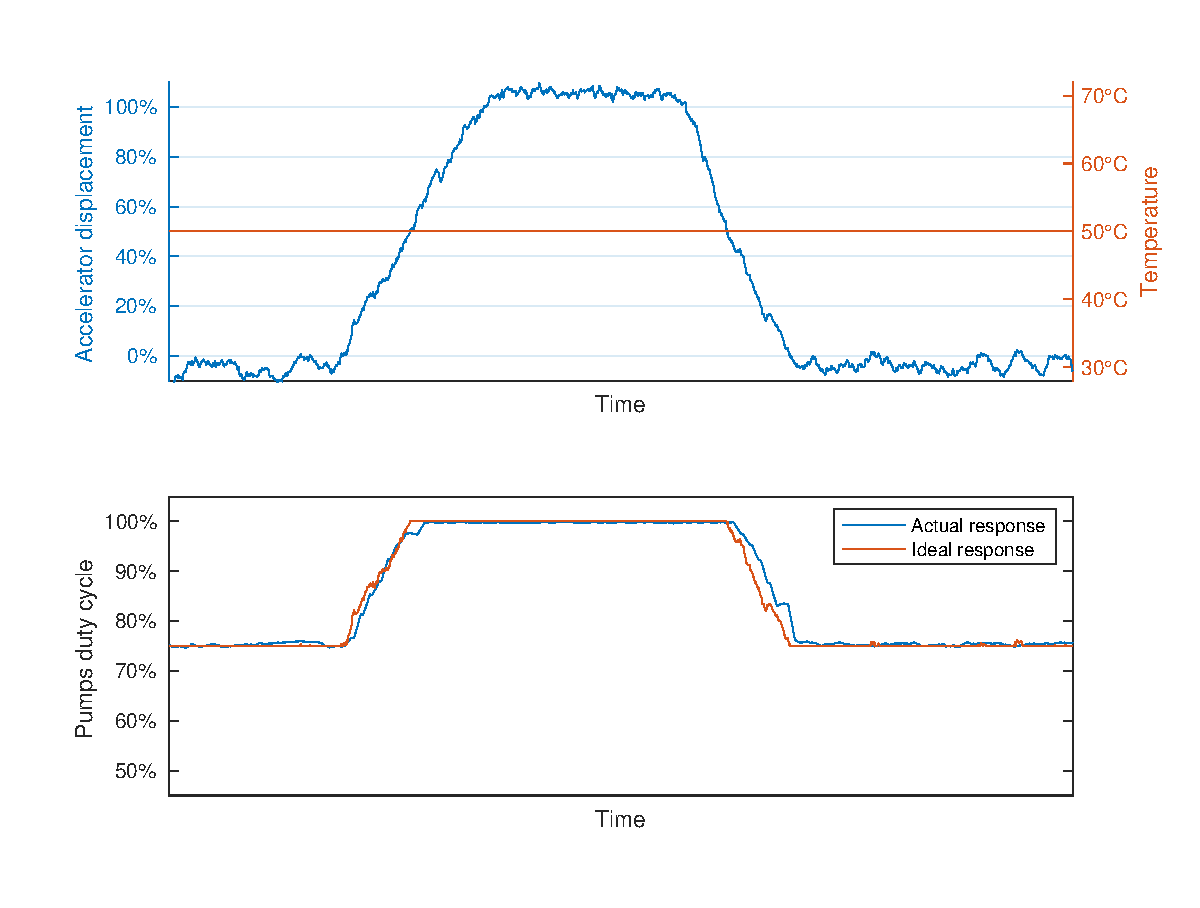
\includegraphics[height=5cm]{figures/pump_50.eps}
            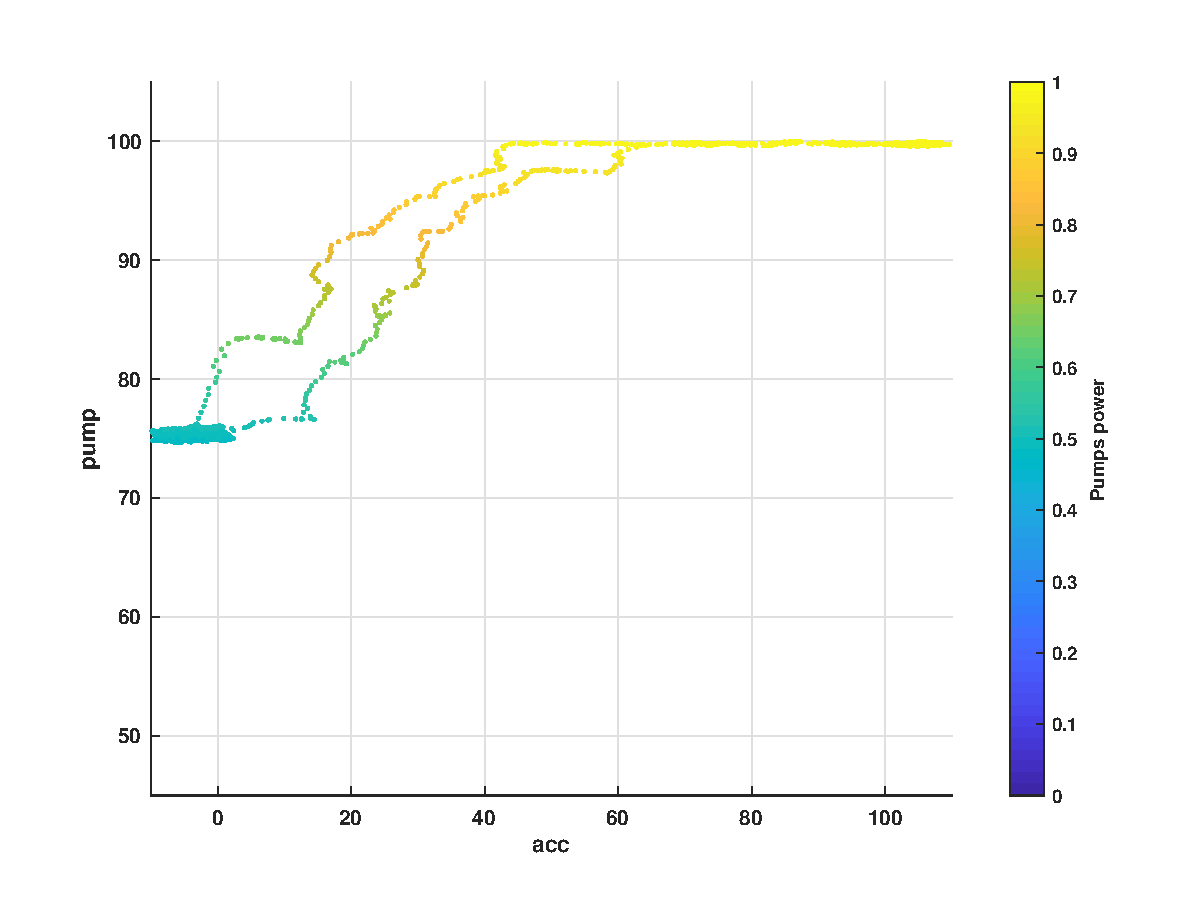
\includegraphics[height=5cm]{figures/pump_50_1.eps}
        }
        ~
        \subbottom[Temperature set to 70\textdegree C and varying accelerator displacement]{
            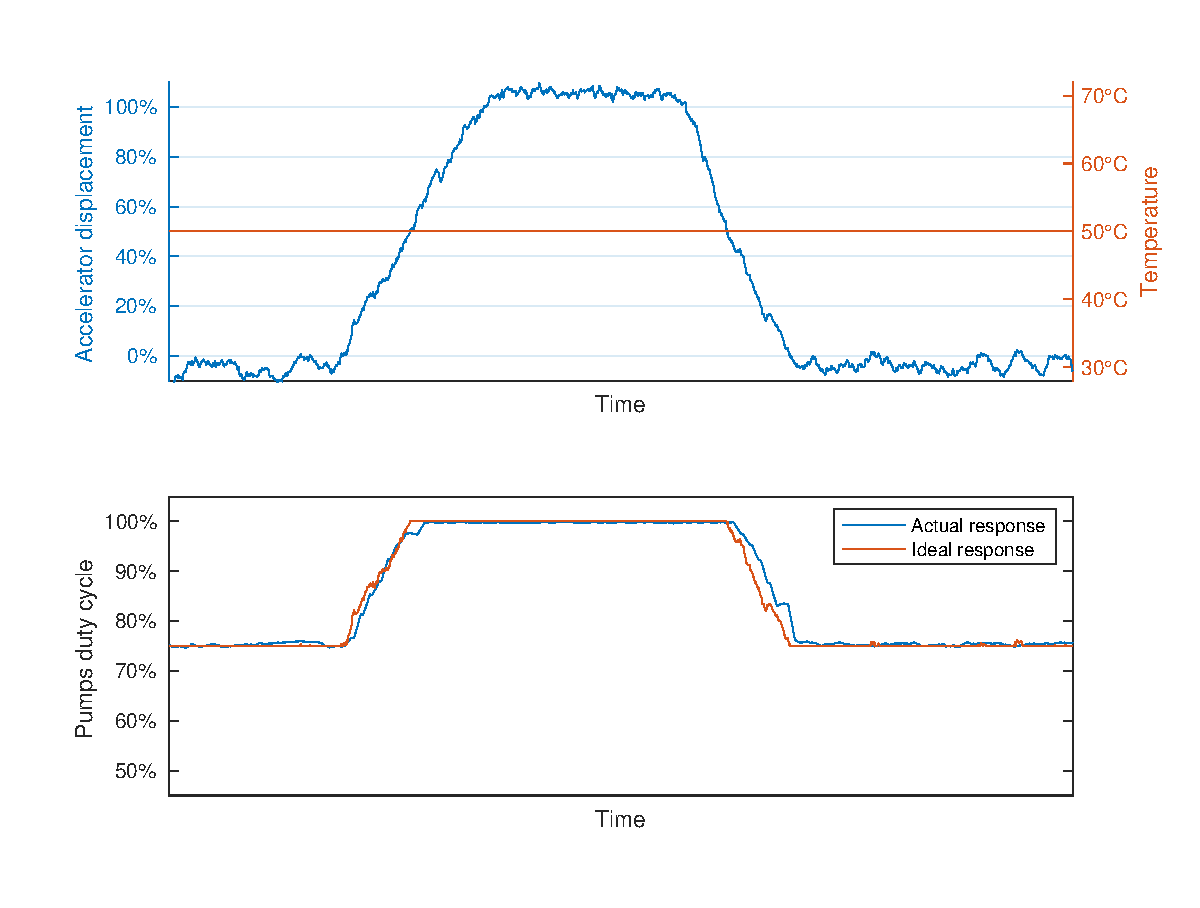
\includegraphics[height=5cm]{figures/pump_50.eps}
            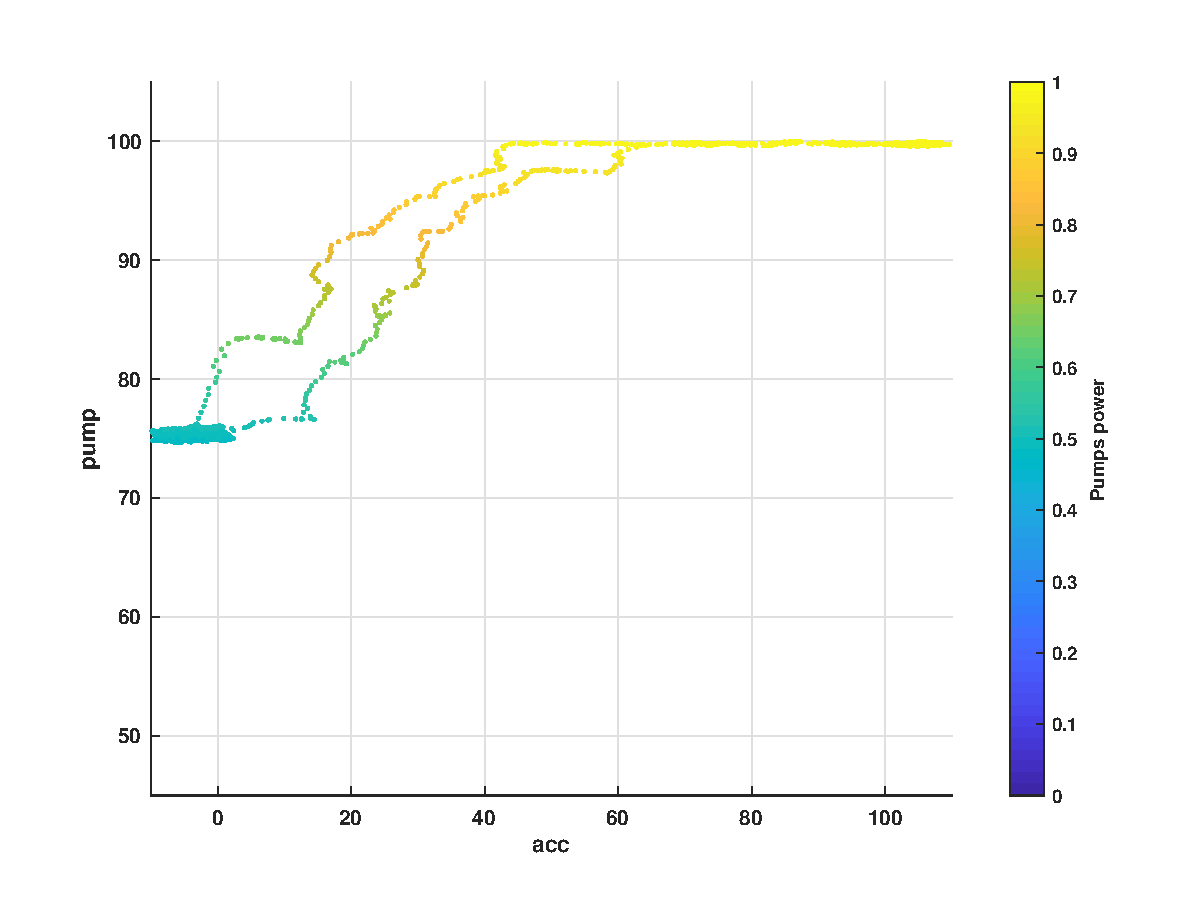
\includegraphics[height=5cm]{figures/pump_50_1.eps}
        }
        ~
        \subbottom[Varying temperature from 30 to 70 degrees and no accelerator displacement]{
            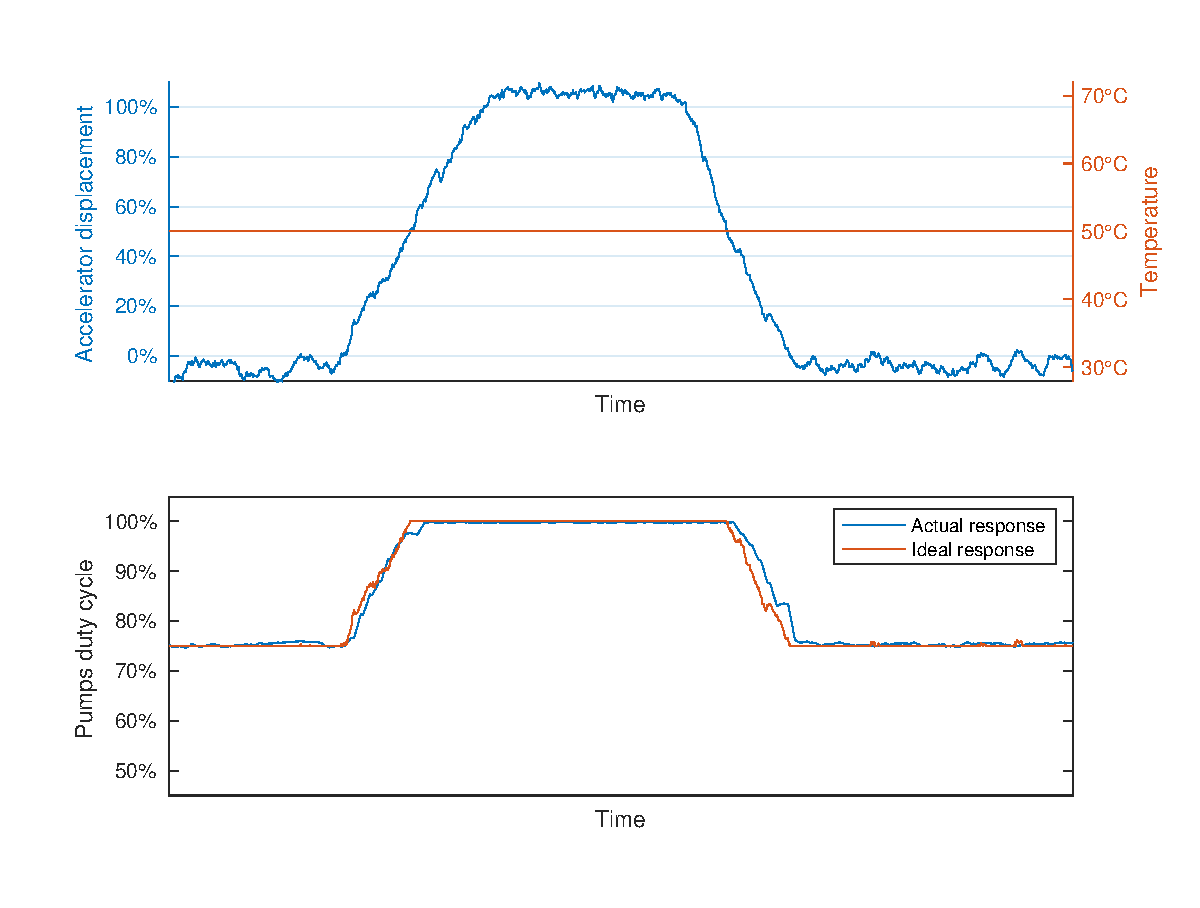
\includegraphics[height=5cm]{figures/pump_50.eps}
            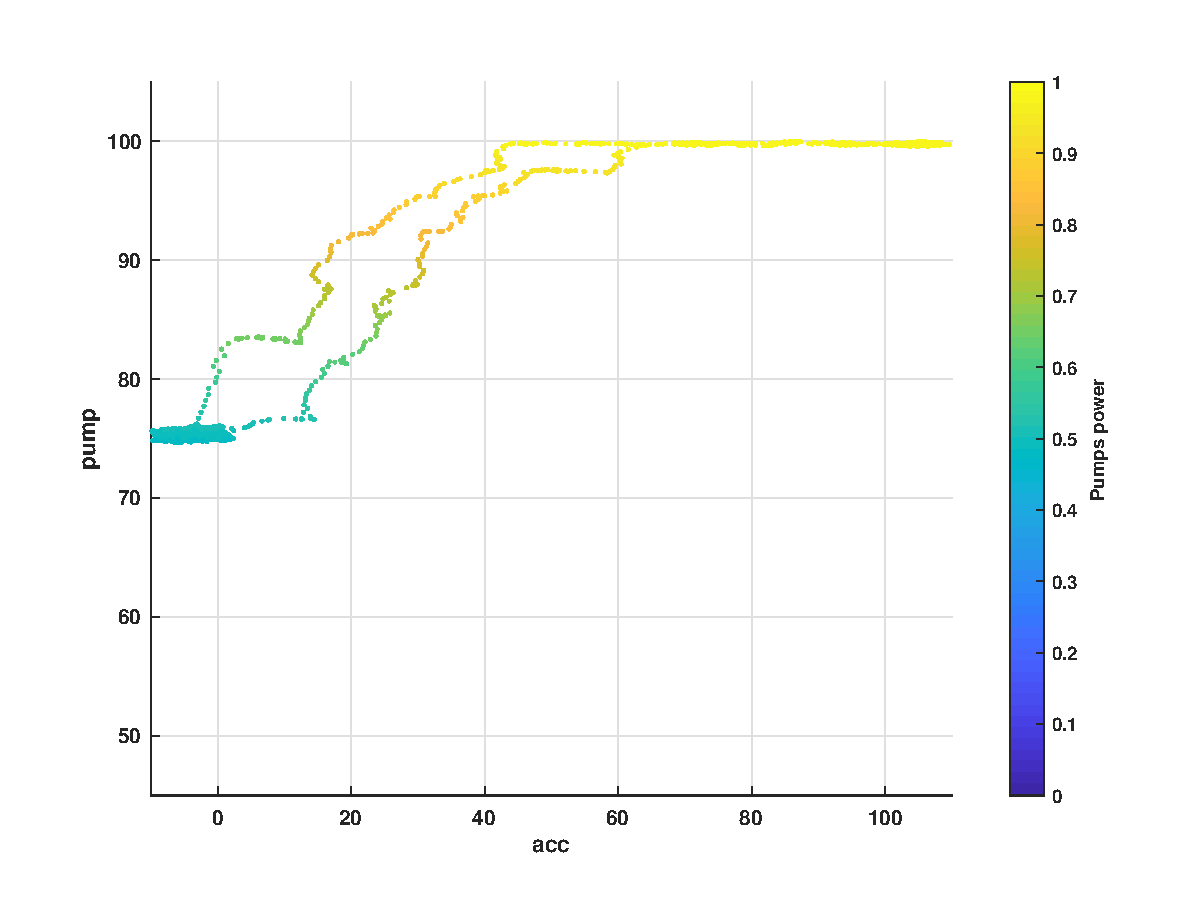
\includegraphics[height=5cm]{figures/pump_50_1.eps}
        }
        % \caption{}
\end{figure}
\let\cleardoublepage\clearpage
\Chapter{}{Differential control measurements}\label{diff_app}
\begin{figure}[h]
    \centering
        \subbottom[Temperature set to 30\textdegree C and varying accelerator displacement]{
            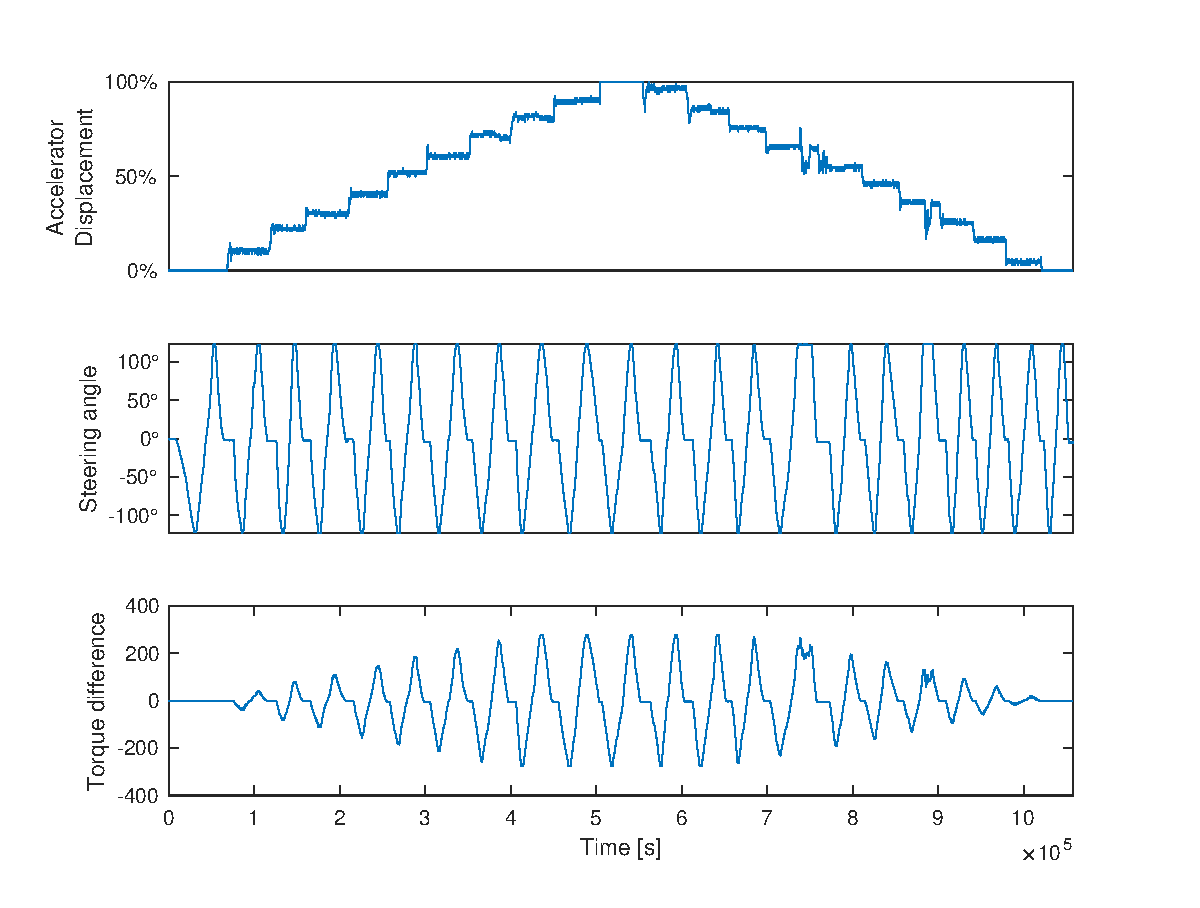
\includegraphics[height=5cm]{figures/vssa.eps}
        }
        ~
        \subbottom[Temperature set to 35\textdegree C and varying accelerator displacement]{
            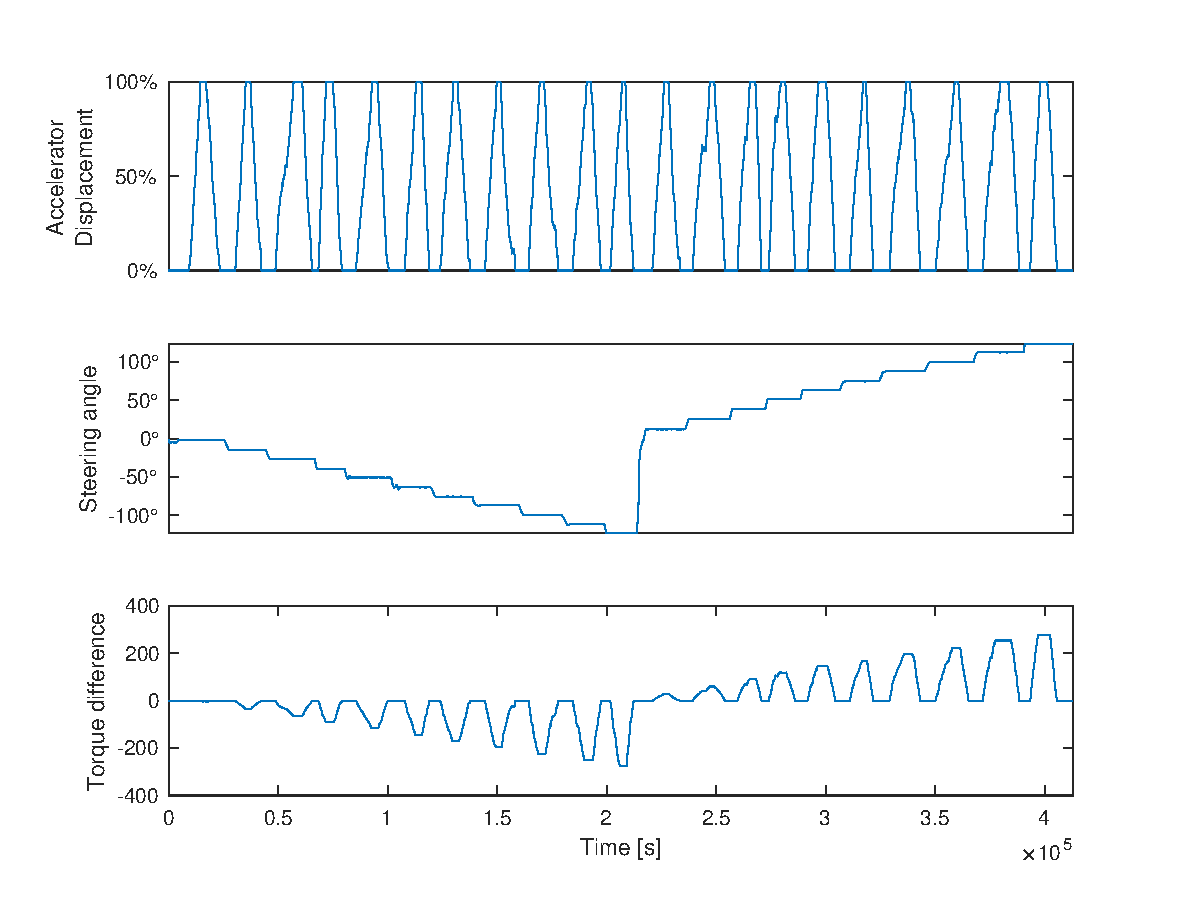
\includegraphics[height=5cm]{figures/ssva.eps}
        }
        % \caption{}
\end{figure}

\backmatter
\printbibliography

\end{document}
